\documentclass[11pt,fleqn]{book} 

\makeatletter
\renewcommand{\p@enumii}[1]{\theenumi#1}
\renewcommand{\p@enumiii}[1]{\theenumi\theenumii#1}
%\renewcommand{\p@enumiv}[1]{\theenumi\theenumii\theenumiii(#1)}
\renewcommand\theenumi{\Alph{enumi}}
\renewcommand\theenumii{\arabic{enumii}}
\renewcommand\theenumiii{\alph{enumiii}}
\renewcommand\theenumiv{\roman{enumiv}}
\renewcommand\labelenumi{\Alph{enumi}.}
\renewcommand\labelenumii{\theenumi\theenumii.}
\renewcommand\labelenumiii{\theenumiii.}
\renewcommand\labelenumiv{(\theenumiv)}

\newcommand\listprocedurename{List of procedures}
\newcommand\listofprocedures{%
    \if@twocolumn
      \@restonecoltrue\onecolumn
    \else
      \@restonecolfalse
    \fi
    \chapter*{\listprocedurename}%
      \@mkboth{\MakeUppercase\listprocedurename}%
              {\MakeUppercase\listprocedurename}%
    \@starttoc{lop}%
    \if@restonecol\twocolumn\fi
}
\newcounter{procedure}[chapter]
\renewcommand\theprocedure{\ifnum \c@chapter>\z@ \thechapter.\fi \@arabic\c@procedure}
\let\l@procedure\l@figure
\def\ext@procedure{lop}

\def\menu#1#2{\texttt{#1}\ifx{}#2\else\@for\@x:=#2\do{$\rightarrow$\texttt{\@x}}\fi}
\def\wmenu#1#2{window menu \menu{#1}{#2}}
\def\mmenu#1#2{left-click mouse menu \menu{#1}{#2}} 
\def\fetchob{\wmenu{File}{Load OBs,From file...}} 


\makeatother
\def\home{\textasciitilde{}}

\newcommand{\procedure}[1]{
\refstepcounter{procedure}
\par\noindent\textbf{Procedure \theprocedure. #1}
\addcontentsline{lop}{procedure}{\protect\numberline{\theprocedure}{\protect\ignorespaces #1}}
\par}

\usepackage[top=3cm,bottom=3cm,left=1.8cm,right=1.8cm,headsep=10pt,a4paper]{geometry} % Page margins

\usepackage{xcolor} % Required for specifying colors by name
\definecolor{ocre}{cmyk}{1,.60,0,.40} % Define the orange color used for highlighting throughout the book

% Font Settings
\usepackage{avant} % Use the Avantgarde font for headings
%\usepackage{times} % Use the Times font for headings
\usepackage{mathptmx} % Use the Adobe Times Roman as the default text font together with math symbols from the Sym­bol, Chancery and Com­puter Modern fonts

\usepackage{microtype} % Slightly tweak font spacing for aesthetics
\usepackage{subfigure}
\usepackage[utf8]{inputenc} % Required for including letters with accents
\usepackage[T1]{fontenc} % Use 8-bit encoding that has 256 glyphs


% Bibliography
%\usepackage[style=alphabetic,sorting=nyt,sortcites=true,autopunct=true,babel=hyphen,hyperref=true,abbreviate=false,backref=true,backend=biber]{biblatex}
%\addbibresource{bibliography.bib} % BibTeX bibliography file
%\defbibheading{bibempty}{}

% Index
\usepackage{calc} % For simpler calculation - used for spacing the index letter headings correctly
\usepackage{makeidx} % Required to make an index
\makeindex % Tells LaTeX to create the files required for indexing


%\usepackage{enumitem}
%\setlist[enumerate,1]{label*=\Alph*.,ref=\Alph*}
%\setlist[enumerate,2]{label*=\arabic*.,ref=\arabic*}
%\setlist[enumerate,3]{label*=\alph*.,ref=\alpha*}
%\setlist[enumerate,4]{label*=\roman*.,ref=\roman*}


%----------------------------------------------------------------------------------------

\makeatletter

\def\abstract#1{\def\@abstract{#1}}
\def\version#1{\def\@version{#1}}

%%%%%%%%%%%%
% graphics %
%%%%%%%%%%%%
\usepackage{graphicx}
\graphicspath{{Pictures/}}

%%%%%%%%%%%%%%
% basic typo %
%%%%%%%%%%%%%%

% colours
\usepackage{xcolor}
\definecolor{ocre}{cmyk}{1,.60,0,.40}

% fonts & endcoding
\usepackage{avant}
\usepackage{mathptmx} 
\usepackage{microtype} % Slightly tweak font spacing for aesthetics
\usepackage[utf8]{inputenc} % Required for including letters with accents
\usepackage[T1]{fontenc} % Use 8-bit encoding that has 256 glyphs

%%%%%%%%%%%
% Figures %
%%%%%%%%%%% 

\usepackage{subfigure}

% reference to figures
\def\figref#1{Fig.~\ref{fig:#1}, p.~\pageref{fig:#1}}
\def\figureref#1{Figure.~\ref{fig:#1}, p.~\pageref{fig:#1}}


%%%%%%%%%%%%%%
% Procedures %
%%%%%%%%%%%%%%

% list of procedures
\newcommand\listprocedurename{List of procedures}
\newcommand\listofprocedures{%
    \if@twocolumn
      \@restonecoltrue\onecolumn
    \else
      \@restonecolfalse
    \fi
    \chapter*{\listprocedurename}%
      \@mkboth{\MakeUppercase\listprocedurename}%
              {\MakeUppercase\listprocedurename}%
    \@starttoc{lop}%
    \if@restonecol\twocolumn\fi
}

% procedure counter
\newcounter{procedure}[chapter]
\renewcommand\theprocedure{\ifnum \c@chapter>\z@ \thechapter.\fi \@arabic\c@procedure}
\let\l@procedure\l@figure
\def\ext@procedure{lop}

% procedure non-float
\newcommand{\procedure}[1]{
\refstepcounter{procedure}
\par\noindent\textbf{Procedure \theprocedure. #1}
\addcontentsline{lop}{procedure}{\protect\numberline{\theprocedure}{\protect\ignorespaces #1}}
\par}

% reference to procedures
\def\procref#1{Procedure~\ref{proc:#1}, p.~\pageref{proc:#1}}

%%%%%%%%%%%%%%%%%%%%
% Various packages %
%%%%%%%%%%%%%%%%%%%%

\usepackage{titlesec} % Allows customization of titles


\usepackage{lipsum} % Inserts dummy text

\usepackage{tikz} % Required for drawing custom shapes


%%%%%%%%%%%%%%%%%%%%%%%%%%
% Lists and enumerations %
%%%%%%%%%%%%%%%%%%%%%%%%%%

% reduce spacing between items
\usepackage{enumitem} 
\setlist{nolistsep} 

% convenient numbering of deeply nested enumerations
\renewcommand{\p@enumii}[1]{\theenumi#1}
\renewcommand{\p@enumiii}[1]{\theenumi\theenumii#1}
%\renewcommand{\p@enumiv}[1]{\theenumi\theenumii\theenumiii(#1)}
\renewcommand\theenumi{\Alph{enumi}}
\renewcommand\theenumii{\arabic{enumii}}
\renewcommand\theenumiii{\alph{enumiii}}
\renewcommand\theenumiv{\roman{enumiv}}
\renewcommand\labelenumi{\Alph{enumi}.}
\renewcommand\labelenumii{\theenumi\theenumii.}
\renewcommand\labelenumiii{\theenumiii.}
\renewcommand\labelenumiv{(\theenumiv)}
\usepackage{booktabs} % Required for nicer horizontal rules in tables

\usepackage{eso-pic} % Required for specifying an image background in the title page

%%%%%%%%%%%%%%%%%%%%%
% Table of contents %
%%%%%%%%%%%%%%%%%%%%%

%
% Proper number alignment in lists of and toc
%
\def\numberline#1{\parbox[t]{3em}{#1}}

%
% Main toc
% 
\usepackage{titletoc} 

\contentsmargin{0cm} % Removes the default margin
% Chapter text styling
\titlecontents{chapter}[1.25cm] % Indentation
{\addvspace{15pt}\large\sffamily\bfseries} % Spacing and font options for chapters
{\color{ocre!60}\contentslabel[\Large\thecontentslabel]{1.25cm}\color{ocre}} % Chapter number
{}  
{\color{ocre!60}\normalsize\sffamily\bfseries\;\titlerule*[.5pc]{.}\;\thecontentspage} % Page number
% Section text styling
\titlecontents{section}[1.25cm] % Indentation
{\addvspace{5pt}\sffamily\bfseries} % Spacing and font options for sections
{\contentslabel[\thecontentslabel]{1.25cm}} % Section number
{}
{\sffamily\hfill\color{black}\thecontentspage} % Page number
[]
% Subsection text styling
\titlecontents{subsection}[1.25cm] % Indentation
{\addvspace{1pt}\sffamily\small} % Spacing and font options for subsections
{\contentslabel[\thecontentslabel]{1.25cm}} % Subsection number
{}
{\sffamily\;\titlerule*[.5pc]{.}\;\thecontentspage} % Page number
[] 

% Minitoc for each chapter

\titlecontents{lsection}[0em] % Indendating
{\footnotesize\sffamily} % Font settings
{}
{}
{}

% Subsection text styling
\titlecontents{lsubsection}[.5em] % Indentation
{\normalfont\footnotesize\sffamily} % Font settings
{}
{}
{}

%%%%%%%%%%%%%%%% 
% Page headers %
%%%%%%%%%%%%%%%% 

\usepackage{fancyhdr} % Required for header and footer configuration

\pagestyle{fancy}
\renewcommand{\chaptermark}[1]{\markboth{\sffamily\normalsize\thechapter\hspace{5 pt}#1}{}} 
\renewcommand{\sectionmark}[1]{\markright{\sffamily\normalsize\thesection\hspace{5pt}#1}{}} 
\fancyhf{} 
\fancyhead[LE,RO]{\sffamily\normalsize\thepage} 
\fancyhead[LO]{\rightmark} 
\fancyhead[RE]{\leftmark} 
\renewcommand{\headrulewidth}{0.5pt} % Width of the rule under the header
\addtolength{\headheight}{2.5pt} % Increase the spacing around the header slightly
\renewcommand{\footrulewidth}{0pt} % Removes the rule in the footer
\fancypagestyle{plain}{\fancyhead{}\renewcommand{\headrulewidth}{0pt}} % Style for when a plain pagestyle is specified

% Removes the header from odd empty pages at the end of chapters
\renewcommand{\cleardoublepage}{
\clearpage\ifodd\c@page\else
\hbox{}
\vspace*{\fill}
\thispagestyle{empty}
\newpage
\fi}

%%%%%%%%%%%%
% Sections % 
%%%%%%%%%%%%

% reference to sections
\def\secref#1{Sect.~\ref{sec:#1}, p.~\pageref{sec:#1}}

% section numbering in the margin
\renewcommand{\@seccntformat}[1]{\llap{\textcolor{ocre}{\csname the#1\endcsname}\hspace{1em}}}                    
\renewcommand{\section}{\@startsection{section}{1}{\z@}
{-4ex \@plus -1ex \@minus -.4ex}
{1ex \@plus.2ex }
{\normalfont\large\sffamily\bfseries}}
\renewcommand{\subsection}{\@startsection {subsection}{2}{\z@}
{-3ex \@plus -0.1ex \@minus -.4ex}
{0.5ex \@plus.2ex }
{\normalfont\sffamily\bfseries}}
\renewcommand{\subsubsection}{\@startsection {subsubsection}{3}{\z@}
{-2ex \@plus -0.1ex \@minus -.2ex}
{0.2ex \@plus.2ex }
{\normalfont\small\sffamily\bfseries}}                        
\renewcommand\paragraph{\@startsection{paragraph}{4}{\z@}
{-2ex \@plus-.2ex \@minus .2ex}
{0.1ex}
{\normalfont\small\sffamily\bfseries}}

%%%%%%%%%%%%
% Chapters %
%%%%%%%%%%%%

% reference to chapters
\def\chapref#1{Chapter~\ref{chap:#1}, p.~\pageref{chap:#1}}

% headings
\newcommand{\thechapterimage}{}
\newcommand{\chapterimage}[1]{\renewcommand{\thechapterimage}{#1}}
\def\thechapter{\arabic{chapter}}
\def\@makechapterhead#1{
\thispagestyle{empty}
{\centering \normalfont\sffamily
\ifnum \c@secnumdepth >\m@ne
\if@mainmatter
\startcontents
\begin{tikzpicture}[remember picture,overlay]
\node at (current page.north west)
{\begin{tikzpicture}[remember picture,overlay]

\node[anchor=north west,inner sep=0pt] at (0,0) {\includegraphics[width=\paperwidth]{\thechapterimage}};

% minitoc 
\draw[fill=white,opacity=.6] (1cm,0) rectangle (8cm,-7cm);
\node[anchor=north west] at (1cm,.25cm) {\parbox[t][8cm][t]{6.5cm}{\huge\bfseries\flushleft \printcontents{l}{1}{\setcounter{tocdepth}{1}}}};

\draw[anchor=west] (5cm,-9cm) node [rounded corners=25pt,fill=white,fill opacity=.6,text opacity=1,draw=ocre,draw opacity=1,line width=2pt,inner sep=15pt]{\huge\sffamily\bfseries\textcolor{black}{\thechapter\ ---\ #1\vphantom{plPQq}\makebox[22cm]{}}};
\end{tikzpicture}};
\end{tikzpicture}}\par\vspace*{230\p@}
\fi
\fi
}
\def\@makeschapterhead#1{
\thispagestyle{empty}
{\centering \normalfont\sffamily
\ifnum \c@secnumdepth >\m@ne
\if@mainmatter
\startcontents
\begin{tikzpicture}[remember picture,overlay]
\node at (current page.north west)
{\begin{tikzpicture}[remember picture,overlay]
\node[anchor=north west] at (-4pt,4pt) {\includegraphics[width=\paperwidth]{\thechapterimage}};
\draw[anchor=west] (5cm,-9cm) node [rounded corners=25pt,fill=white,opacity=.7,inner sep=15.5pt]{\huge\sffamily\bfseries\textcolor{black}{\vphantom{plPQq}\makebox[22cm]{}}};
\draw[anchor=west] (5cm,-9cm) node [rounded corners=25pt,draw=ocre,line width=2pt,inner sep=15pt]{\huge\sffamily\bfseries\textcolor{black}{#1\vphantom{plPQq}\makebox[22cm]{}}};
\end{tikzpicture}};
\end{tikzpicture}}\par\vspace*{230\p@}
\fi
\fi
}

%%%%%%%%%%%%%%
% Title page %
%%%%%%%%%%%%%%

% title page colour & background
\usepackage[some]{background}
\usepackage{lipsum}

\definecolor{titlepagecolor}{cmyk}{1,.60,0,.40}

\DeclareFixedFont{\bigsf}{T1}{phv}{b}{n}{1.5cm}

\backgroundsetup{
scale=1,
angle=0,
opacity=1,
contents={\begin{tikzpicture}[remember picture,overlay]
 \path [fill=titlepagecolor] (-0.5\paperwidth,3) rectangle (0.5\paperwidth,10);  
\end{tikzpicture}}
}

% function to build the page

\def\maketitle{%
\begin{titlepage}
\BgThispage
\vspace*{6cm}
\noindent
\textcolor{white}{\huge\textsf{\@title}}
\vspace*{2.5cm}\par
\noindent
\begin{minipage}{0.35\linewidth}
    {\large\@author}
\end{minipage}\hspace{0.04\linewidth}%
\begin{minipage}{0.01\linewidth}
    \color{ocre}\rule{\linewidth}{190pt}
\end{minipage}\hspace{0.04\linewidth}%
\begin{minipage}{0.56\linewidth}
\@abstract\\[2ex]
Version: \@version.
\end{minipage}%
\end{titlepage}
\restoregeometry
%
\chapterimage{lasilla.pdf}% Chapter heading image
}

\makeatother
 % Insert the commands.tex file which contains the majority of the structure behind the template

\usepackage[pdftex,colorlinks=true,linkcolor=ocre]{hyperref}
\usepackage[all]{hypcap}

\usepackage{glossaries}
\renewcommand*{\glspostdescription}{}
\makeglossaries
\newacronym[sort=bob]{bob}{\texttt{bob}}{broker for observing blocks}
\newacronym{drs}{DRS}{data reduction software}
\newacronym[sort=ot]{ot}{\texttt{ot}}{observing tool}
\newacronym[sort=p2pp]{p2pp}{\texttt{p2pp}}{phase 2 preparation tool}
\newacronym{ob}{OB}{observing block}
\newacronym{tcs}{TCS}{telescope control software}
\newacronym{ics}{ICS}{instrument control software}
\newacronym{adc}{ADC}{atmospheric diffraction corrector}
\newacronym{rtd}{RTD}{real time display}
\newacronym{ag}{AG}{autoguider}
\newacronym{wfi}{WFI}{wide-field imager}
\newacronym{grond}{GROND}{Gamma-Ray Burst Optical/Near-Infrared Detector}
\newacronym{feros}{FEROS}{Fibre-fed Extended Range Optical Spectrograph}
\newglossaryentry{lcu}{name=LCU,description={Logical control unit, machine in a rack that controls an instrument or telescope subsystem}}
\newglossaryentry{windows}{name=Windows desktop,description={Rightmost computer in the control room that controls the dome}}
\newglossaryentry{adam}{name=ADAM,description={Telescope hydraulics and mirror cover control system}}
\newglossaryentry{midas}{name=MIDAS,description={The well known reduction software}}
\newglossaryentry{fiera}{name=FIERA,description={Electronics systems controlling the optical detectors}}
\newglossaryentry{irace}{name=IRACE,description={Electronics systems controlling the infrared detectors.}}
\newglossaryentry{auxfunc}{name=Auxiliary Functions,description={Panel with cryptic title \texttt{E2P2FAUX PANEL} (Fig.~\ref{fig:tcsauxfunc}) controlling WFI shutter and flat-field lamp.}}
\newglossaryentry{webcam}{name=dome webcam,description={View into the dome given by the \texttt{TRENDNET} tab of mozilla on the \gls{windows}.}}
\newglossaryentry{domefunc}{name=Dome Auxiliary Functions,description={\texttt{ADAM 6000} tab of mozilla on the \gls{windows} that contains hydraulics and ventilation control of the dome.}}
\parindent=0pt
\parskip=1ex

\usepackage{amsmath}
\usepackage[some]{background}
\usepackage{lipsum}

\definecolor{titlepagecolor}{cmyk}{1,.60,0,.40}

\DeclareFixedFont{\bigsf}{T1}{phv}{b}{n}{1.5cm}

\backgroundsetup{
scale=1,
angle=0,
opacity=1,
contents={\begin{tikzpicture}[remember picture,overlay]
 \path [fill=titlepagecolor] (-0.5\paperwidth,3) rectangle (0.5\paperwidth,10);  
\end{tikzpicture}}
}
\makeatletter                       
\def\printauthor{%                  
    {\large \@author}}              
\makeatother
\author{%
    Rodolfo~Angeloni\vspace{6pt}\\
    Paul~Eigenthaler\\
    \texttt{paul.eigenthaler@icloud.com}\vspace{6pt}\\
    Angela~Hempel\\
    \texttt{ang.hmpl@gmail.com}\vspace{6pt} \\
    Sam~Kim\\
    \texttt{skim@astro.puc.cl}\vspace{6pt} \\
    Iv\'an~Lacerna\vspace{6pt}\\
    R\'egis~Lachaume\\
    \texttt{lachaume@astro.puc.cl}\vspace{6pt} \\
    Markus~Rabus\\
    }

\begin{document}
\begin{titlepage}
\BgThispage
\newgeometry{left=1.8cm,right=1.8cm}
\vspace*{6cm}
\noindent
\textcolor{white}{\huge\textsf{Operations at the La Silla 2.2\,metres telescope}}
\vspace*{2.5cm}\par
\noindent
\begin{minipage}{0.35\linewidth}
    %\begin{flushright}
        \printauthor
    %\end{flushright}
\end{minipage}\hspace{0.04\linewidth}%
\begin{minipage}{0.01\linewidth}
    \color{ocre}\rule{\linewidth}{190pt}
\end{minipage}\hspace{0.04\linewidth}%
\begin{minipage}{0.56\linewidth}
Since 2013, the operations at the La Silla 2.2~metres telescope involve
minimal support by ESO.  This guide intends to familiarise observers with 
the operations.\\[2ex]
Version: \today.
\end{minipage}%
\end{titlepage}
\restoregeometry



%----------------------------------------------------------------------------------------
%	TABLE OF CONTENTS
%----------------------------------------------------------------------------------------
\chapterimage{lasilla.pdf} % Chapter heading image

\tableofcontents % Print the table of contents itself
\cleardoublepage % Forces the first chapter to start on an odd page so it's on the right

\addcontentsline{toc}{chapter}{\listfigurename}
\listoffigures 
\cleardoublepage % Forces the first chapter to start on an odd page so it's on the right

\addcontentsline{toc}{chapter}{\listtablename}
\listoftables
\cleardoublepage % Forces the first chapter to start on an odd page so it's on the right

\addcontentsline{toc}{chapter}{\listprocedurename}
\listofprocedures
\cleardoublepage


%----------------------------------------------------------------------------------------
\chapter{Introduction}
The operational scheme at the La Silla 2.2~metres telescope involves minimal support by ESO.  This guide intends to familiarise observers with the operations. 

\section{Control room}

First of all, the control room, is located below the main ESO building, the one with the dining room.  It is still shared with the two ESO telescopes, the NTT and the 3.6\,m. If everything works without technical issue, you can do everything from there without any need to access the telescope building.

Figure~\ref{fig:saladecontrol}  below shows the location of the different components of the controls.  Screens, keyboards, and mice are labeled to avoid confusion.

\begin{figure}[!ht] 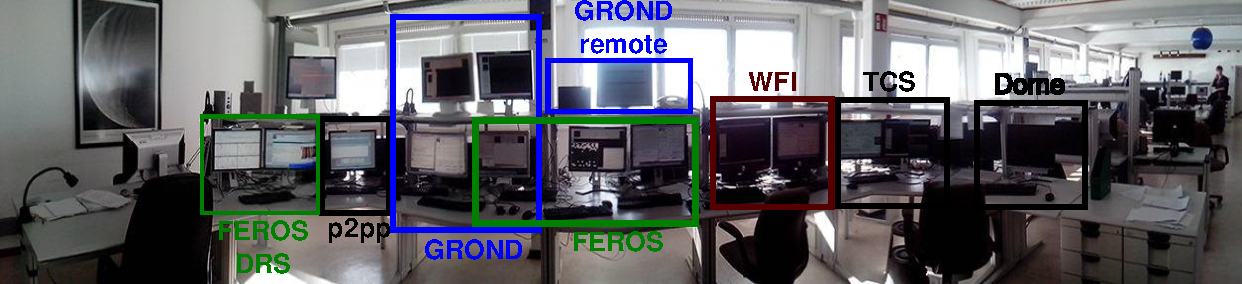
\includegraphics[width=\linewidth]{saladecontrol.pdf}
\caption[Layout of the telescope controls]{Layout of the telescope controls.  From right to left: \gls{windows} 
controlling and monitoring the dome, \acrlong{tcs}, \acrshort{wfi} controls,
\acrshort{feros} controls (bottom) and skype laptop connected to the \acrshort{grond}
remote observers (top), GROND controls, \acrshort{p2pp} machine where
\acrshort{ob}s are crafted and loaded by the visiting astronomer, and,
finally, the FEROS \acrlong{drs}.}
\label{fig:saladecontrol} 
\end{figure}

\section{Overview of operations}

In most nights, a support astronomer is present in the afternoon and the first part of the night, freeing the visitor of the afternoon and evening twilight calibration duties.  Sometimes visitors are ask to perform all duties alone.  In that case, an experienced observer can start operations 2.5 hours before sunset to minimise working time, while giving a small time buffer to solve the commonest technical issues.  Inexperienced ones should plan to start earlier or accept possible downtime in the very beginning of the night. Figure~\ref{fig:timeflow} shows a time-optimised chart of operations in the afternoon and both twilights.

\begin{figure}[!ht]
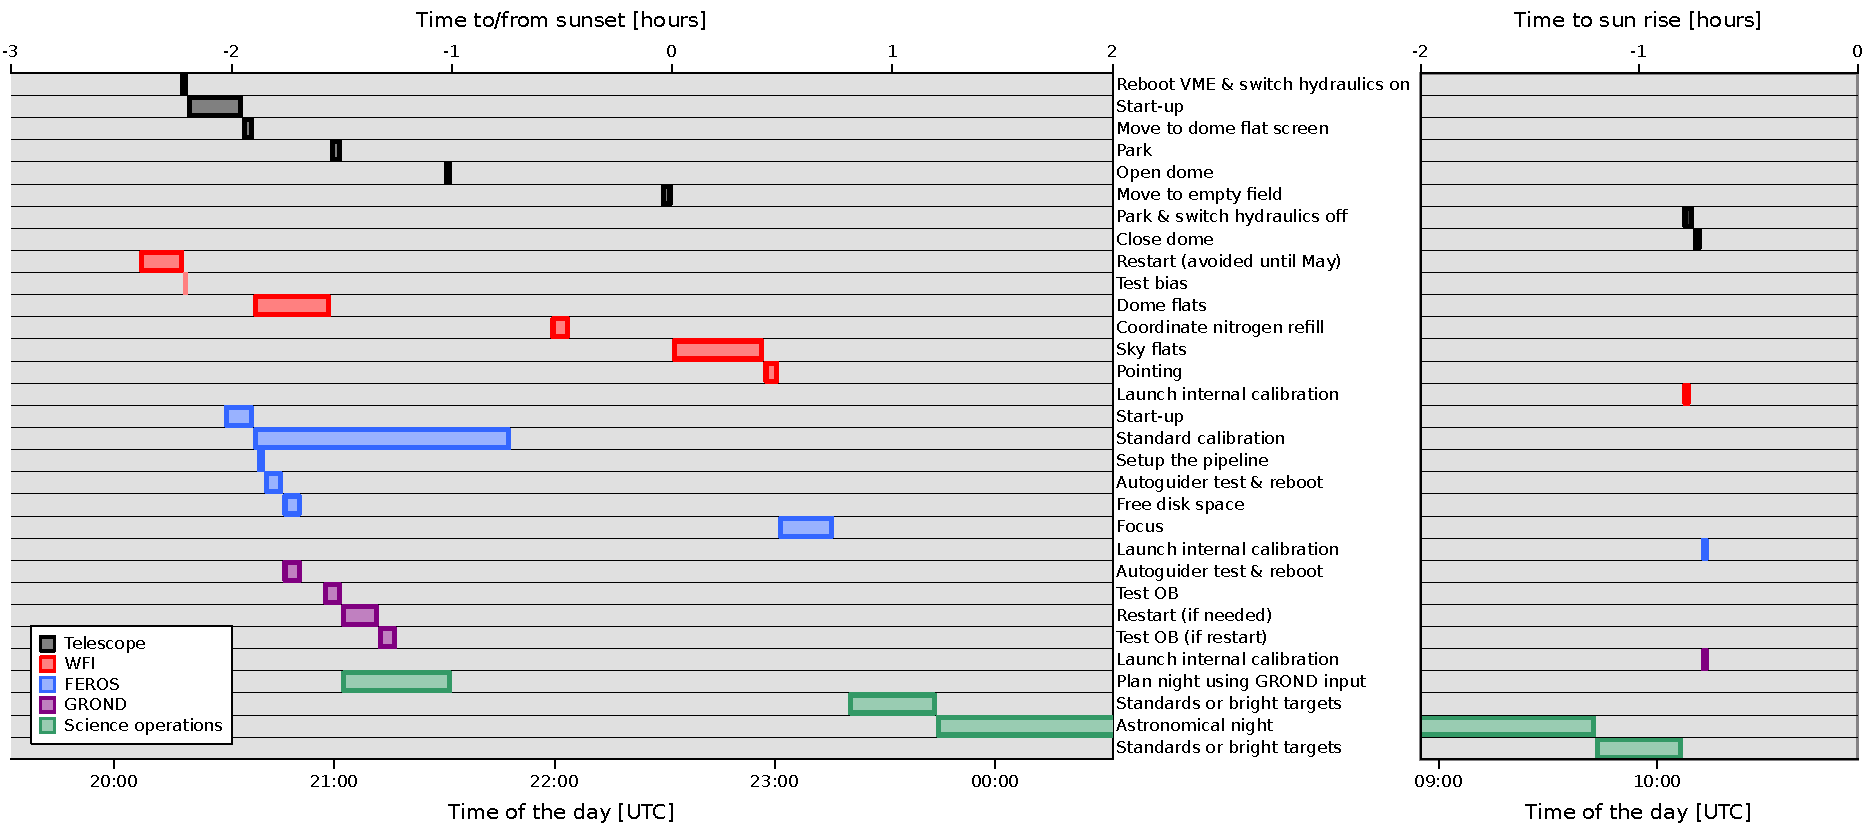
\includegraphics[width=\linewidth]{operations-time-flow.pdf}
\caption{Time flow of operations in the afternoon and twilights. Afternoon setup and calibrations should be started at least 2.5 hours before sunset to leave a small buffer for technical issues. This example is giving for a late fall night (May 15th), with presence required for about 15~hours.}
\label{fig:timeflow}
\end{figure}

When no service astronomer is present (e.g. last part of the night), visiting astronomers will be asked to perform service observations for other groups, both for the follow-up of gamma-ray bursts and time-domain programmes.  The number of allocated nights for visitors takes the average time loss into account, in case more down time, compensation will be considered in service mode.  Since 2017, a long-term monitoring of quasi-stellar objects takes 1.5 to 2 hours daily, and targets of opportunity about 1 hour (15\% long-term average).  MPIA observers may be ask for additional service observations for the MPIA.

Sections~\ref{startup}--\ref{nightops} can be seen as a step-by-step guide of the operations from the daily startup to the night time. Many of the steps need some knowledge of the \gls{ob} management and of the \gls{bob} interface, which
are presented in Section~\ref{ob}.  Section~\ref{sec:trouble} lists fixes to common issues at the telescope.  We present the software components more in detail in Section~\ref{compo}.

\section{Security}

The main guidelines to avoid bodily harm are:
\begin{itemize}
\item Don't move the telescope or dome before checking no one is in the way.  During the day, ESO technicians may address some issues or refill the instrument with nitrogen.  If you operate from the remote control room, check the dome webcam.
\item If you need to go to the dome, leave a conspicuous message in the control room and put the telescope in local control from the computer room of the telescope building.
\item If you drive by night, go very slowly and defensively as you may not see a pedestrian or a dark donkey.  
\item If you walk, take the incoming traffic side and be very careful at night. Drivers don't use lights.
\end{itemize}

ESO has the duty to ensure telescope safety but you have to be proactive, too.  In particular:
\begin{itemize}
\item If you are not able to close when you must (sunrise and inclement weather), you need to ask to the operators present at the NTT or the 3.6m. They have the duty to assist.  
\item The weather officer or the NTT operator will tell you when you need to close and when you may reopen, stick to it.
\item If you have any doubts whether you may open in the afternoon, wait for the NTT to open or ask the ESO day-time operator.
\item If the meteo monitor shows that the closing limits are reached (wind, humidity, clouds), close.
\item If a sea of clouds below the observatory was present at sunset, be attentive as it is common for them to raise and increase humidity to 100\% within minutes.
\end{itemize}

\section{Telescope building}

It is sometimes necessary to physically access the telescope building where there is an old control room (Fig.~\ref{fig:old-control-room}), a computer room to physically access some relevant workstations (Fig.~\ref{fig:computer-room}), the FEROS room, and, obviously, the dome (Fig.~\ref{fig:dome}).  

Some subsystems are controlled by machines gathered in big rack towers, these machines are called \gls{lcu} or sometimes VME.  There are also workstations controlling coordinating with one or more LCUs, they look like a normal desktop computer tower usually with no screen or keyboard.

In the dome itself, many electronic boxes attached at the telescope (see Fig.~\ref{fig:dome}) may need being ``power cycled'', that is switched off and on.  It is also possible to locally take control of telescope, dome, and mirror motion.

\begin{figure}[!ht]
\centering
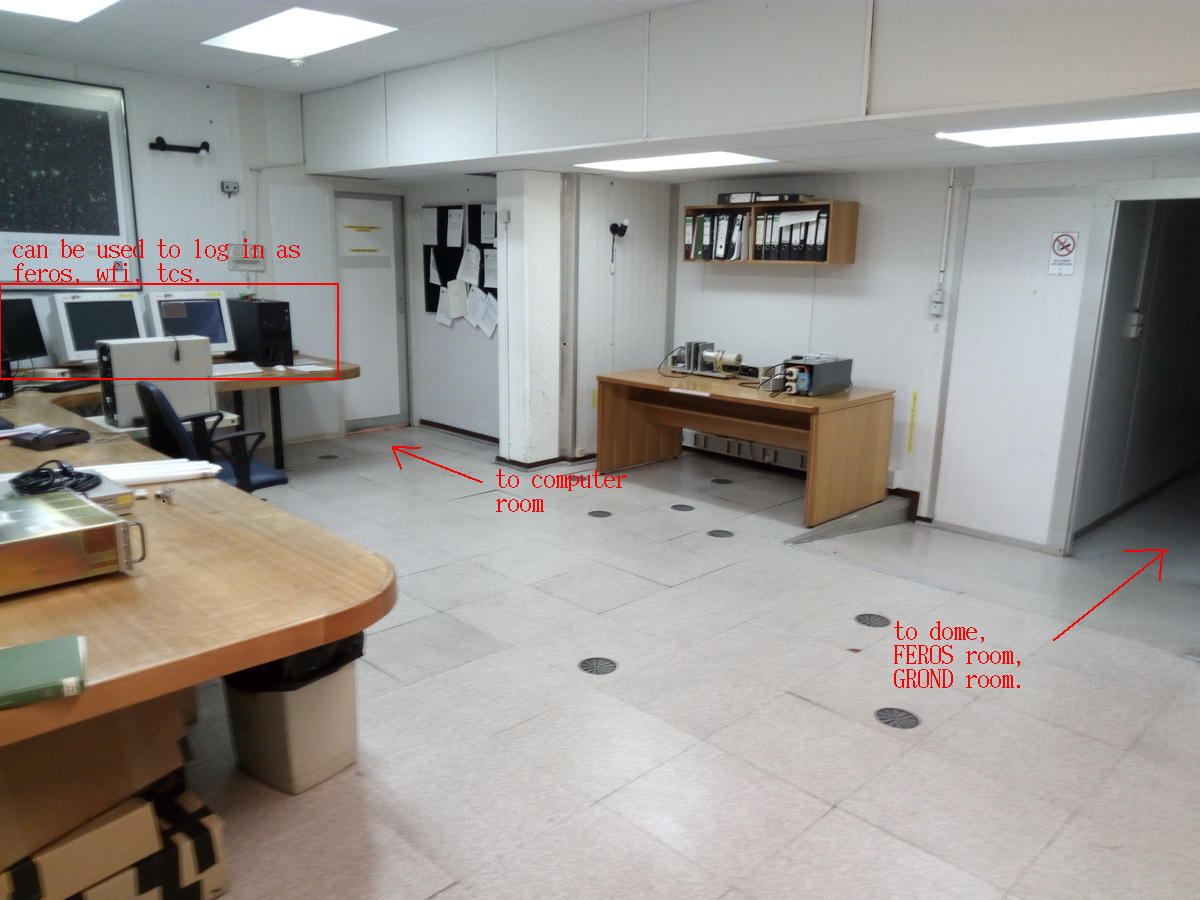
\includegraphics[width=0.7\linewidth]{dome/dome-old-control-room.jpg}
\caption{Entering the old control room in the telescope building}
\label{fig:old-control-room}
\end{figure}

\begin{figure}[!ht]
\centering
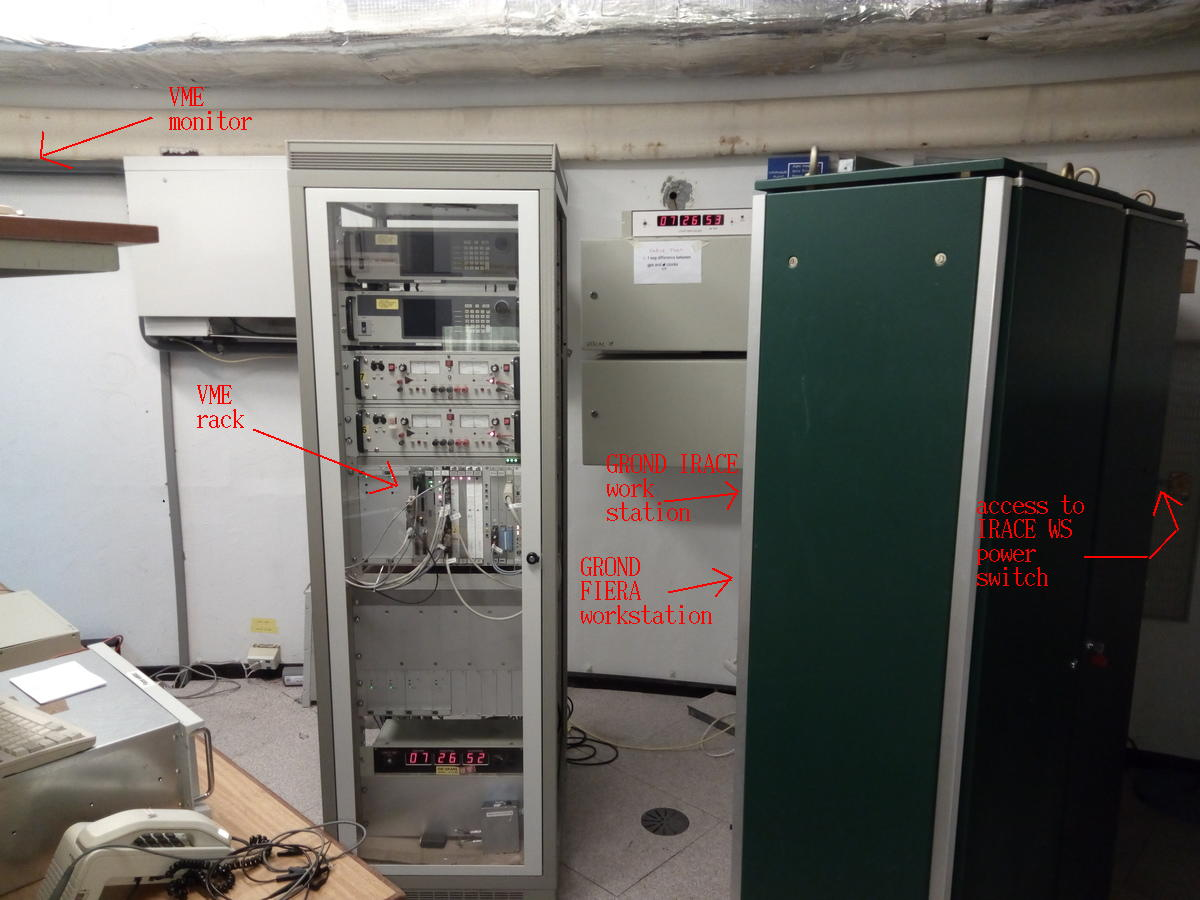
\includegraphics[width=0.7\linewidth]{dome/dome-computer-room.jpg}
\caption[Entering the computer room in the telescope building]{Entering the computer room in the telescope building. In front slightly to the left is the VME rack.} 
\label{fig:computer-room}
\end{figure}

\begin{figure}[!ht]
\centering
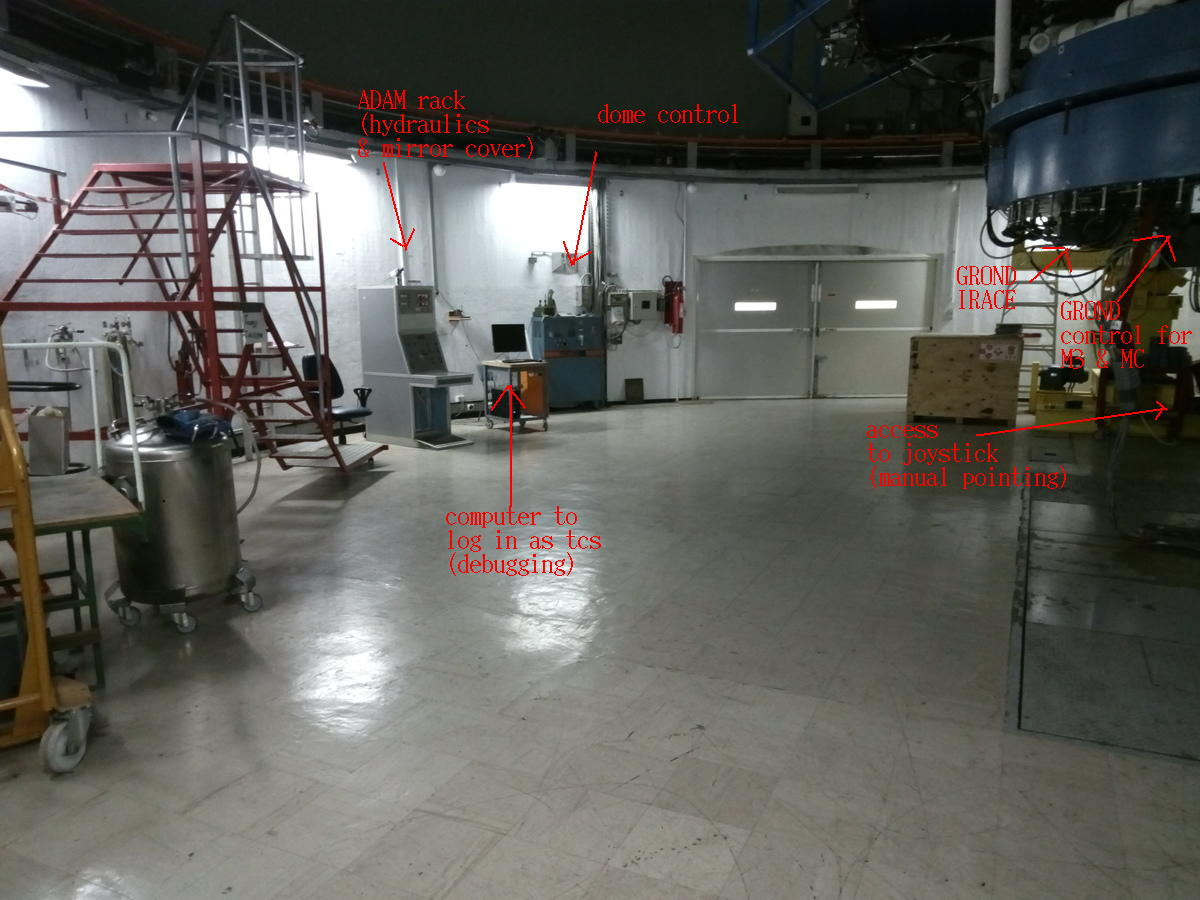
\includegraphics[width=0.7\linewidth]{dome/dome.jpg}
\caption[Entering the dome]{Entering the dome, from left to right: the \gls{adam} controls,
a computer to use the \gls{tcs}, the dome controls, the bottom of the telescope.}
\label{fig:dome}
\end{figure}

\cleardoublepage



%------------------------------------------------------------------------------
%                                       
%                                  
%  DAILY STARTUP
%
%
%------------------------------------------------------------------------------


\chapter{Early afternoon: daily start-up}
\label{startup}

Start-up should take about one hour, but small technical issues can lengthen it significantly.  Ideally, it should be done early enough in the afternoon (2--3 pm in Winter, 3--4 pm in Summer), so that dome flat fields can be done before the nitrogen of \gls{wfi} is refilled.  Also, complicated issues should be diagnosed early, so that you benefit from the day-time support from ESO engineers.  Night time support is not provided except for emergencies.

For an experienced observer alone in Winter, a later start-up can be done by optimising and hoping for the best (see Fig.~\ref{fig:timeflow-eve}), but the risk is to lack time to perform dome flats and/or losing the very beginning of the night to technical issues.

The \gls{tcs} and the \gls{wfi} are entangled.  In particular, the \gls{wfi} \gls{ics} controls the focus and pointing, and the \gls{tcs} controls the \gls{wfi} \gls{ag}.  For this reason, the \gls{wfi} should be rebooted before the \gls{tcs}.  The other instruments, \gls{grond} and \gls{feros}, are more independent and need a later restart. Also, the \gls{feros} and \gls{grond} \gls{ag} should be checked and the \gls{feros} \gls{drs} set to the right date.

\section{Outline}

To be on the safe side, the start-up sequence shall be performed in this order below. To gain a bit more time one can do \ref{list:hydr}--\ref{list:tcs1} during \ref{list:wfi1}--\ref{list:wfibooted} and
\ref{list:tcsboot}--\ref{list:tcsbooted} during
\ref{list:wfiwin}--\ref{list:wfitest}.  \gls{feros}, \gls{grond}, the \gls{ag} and the \gls{drs} (\ref{list:feros}, \ref{list:grond}, \ref{list:ag}, \ref{list:drs}) can be handled in parallel as soon as the \gls{tcs} is booted
(\ref{list:tcsbooted}).  

If under time pressure, you can also do some day-time calibrations in parallel. Figure~\ref{fig:timeflow-eve} gives a time-optimised flow of the day-time start-up and calibrations, showing what can be done in parallel.  It should be started latest 2.5 hours before sunset.
\begin{figure}
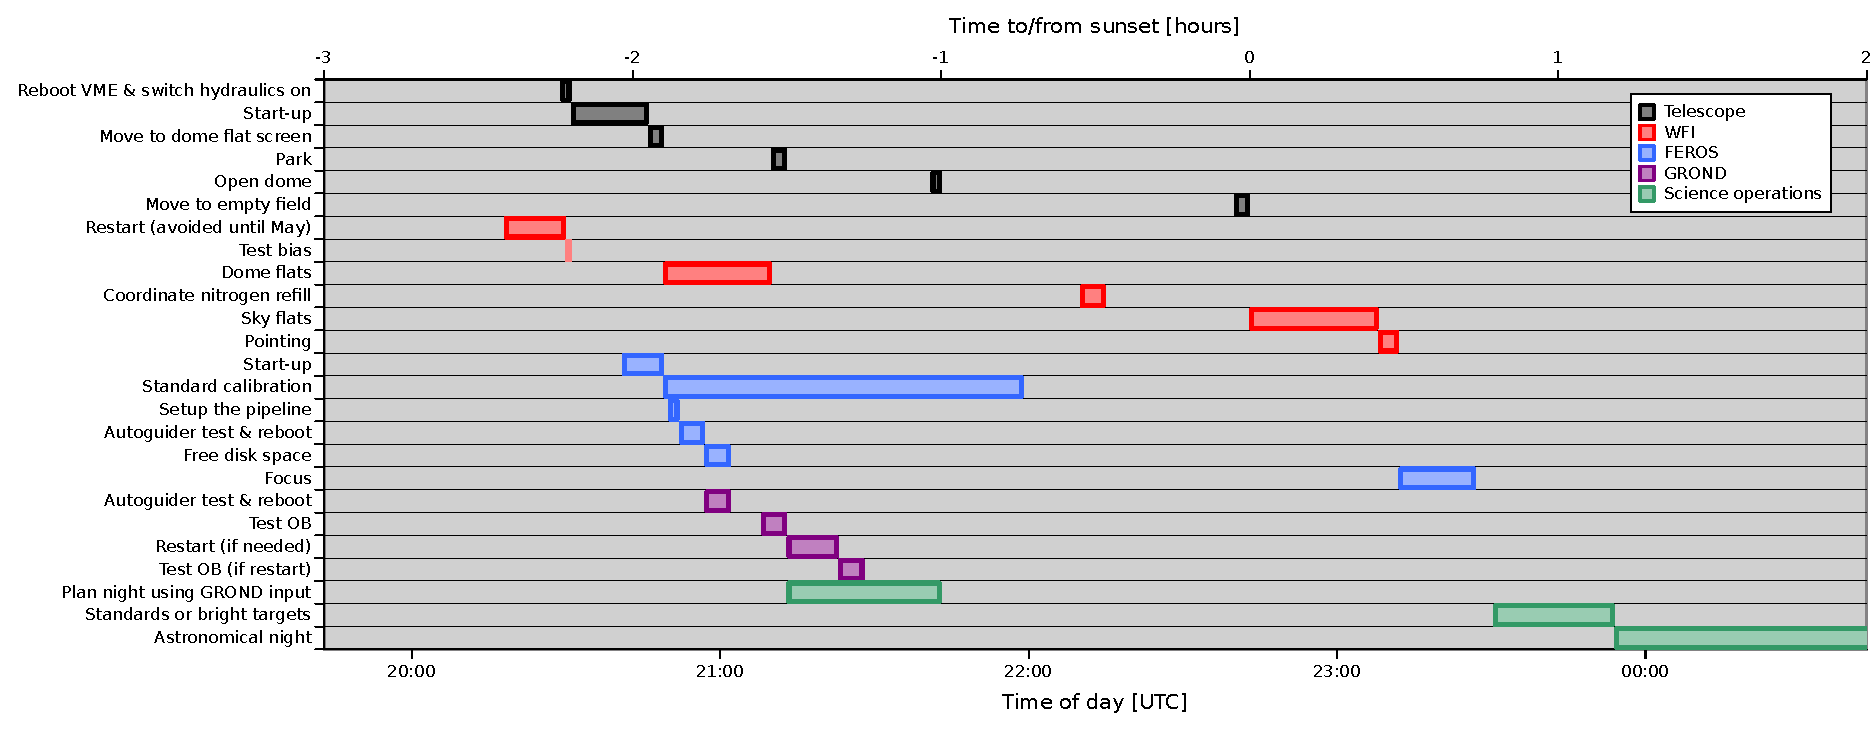
\includegraphics[width=\linewidth]{operations-time-flow-evening.pdf}
\caption{Operations time flow in the evening, doing start-up, calibrations, and tests in parallel.  It should start latest 2.5 hours before sunset (see horizontal axis at the top).  The time of the day, given in universal time on the bottom horizontal axis, corresponds to a date close to fall equinox (September 15th).}
\label{fig:timeflow-eve}
\end{figure}

\procedure{Telescope and instrument startup} 
\label{proc:startup}
\begin{enumerate}
%%%%
%%%% WFI
%%%%
  \item \label{list:wfistartup}\textbf{\gls{wfi} restart (8 min, in case of problems, see Fig.~\ref{fig:wfi-restart})}
        \begin{enumerate}
          \item On the screen \texttt{BOB Wide Field Imager}, go to the \texttt{StartUp} virtual desktop.\label{list:wfi1}
          \item In a terminal, \texttt{osf2p2StartUp ini WFI F8}, where ini is your initials (Fig.~\ref{fig:wfisu-launch}).
          \item On the dialog, choose \texttt{DAILY} startup (Fig.~\ref{fig:wfisu-full}).
          \item Click \texttt{START} on the appearing window (\texttt{ESO220 WEEKLY FULL STARTUP}, see Fig.~\ref{fig:wfisu-start}). 
          \item Wait until the start-up window says \texttt{SCRIPT finished} (about 11 minutes).\\
          A black text window gives indication on the process (Fig.~\ref{fig:wfisu-log})
                \label{list:wfibooted}
          \item Close the startup window (Fig. \ref{fig:wfisu-start})
          \item Close the emerging PDF (Fig.~\ref{fig:wfisu-pdf}).
          \item Rearrange windows to the corresponding desktops (1 min, see Fig.~\ref{fig:wfisu-windows})
             \label{list:wfiwin}
             \begin{itemize}
                \item \gls{rtd} goes to all desktops, on the left screen.
                \item other windows go to the desktop bearing their name, on the right screen. 
            \end{itemize}
          \item Wait for the filtre wheel to be set to a specific filtre (1--2 min)\label{list:wfisu-filtre}
                \begin{enumerate}
                    \item Locate the \texttt{Filter} field on the \texttt{WFI General State} panel
                    \item If it stays in \texttt{MOVING} for more than 2 minutes or you skipped full restart, reset filtre wheel (Procedure~\ref{proc:filtrereset})
                \end{enumerate}
          \item In \gls{bob}, execute \texttt{testOB.obd} (1 min)
             \label{list:wfitest}
             \begin{enumerate}
               \item Import it with \fetchob.
               \item Click the \texttt{Start} button. 
             \end{enumerate}
        \end{enumerate}
%%%%
%%%% TCS
%%%%
  \item \textbf{\gls{tcs} restart (17 min, daily, see Fig.~\ref{fig:tcs-restart})}
        \begin{enumerate}
        \item\label{lab:hydron} Go to web browser on screen \texttt{Dome webcam \& hydraulics} to activate hydraulics (Fig.~\ref{fig:tcssu-hydr}). 
             \begin{enumerate}
               \item Find the \gls{domefunc} (tab called \texttt{ADAM 6000…})\\
                     If it is not there, open it with the bookmark \texttt{Dome controls}.\\
                     Use the good seeing password if necessary.
               \item Click \texttt{HydOn}, then button \texttt{Hydr} goes green.
               \item Click \texttt{DrivesOn}, then button \texttt{Drives} goes green.
             \end{enumerate}
             It may be needed to click two or three times to get green buttons.
             \label{list:hydr}
          \item On the screen \texttt{Telescope Control Software}, go the the \texttt{StartUp} virtual desktop.\label{list:tcs1}
          \item If a \texttt{Cannot read "@w2p2wfi…"} pop-up can be seen on the \gls{tcs} screen (Fig.~\ref{fig:tcssu-error}), click \texttt{OK}.
          \item In a terminal type \texttt{lccBoot lte2p2} and wait for command to end (2 min, Fig.~\ref{fig:tcssu-boot})\\
                If none is there, you can open one with \mmenu{TCS User}{tcs xterm}.\\
                If an error message appears on the \gls{wfi} screen, click \texttt{OK}. 
          \item On the \gls{tcs} screen, type \texttt{osf2p2StartUp ini ALL F8}, where ini is your initials.\label{list:tcsboot} (Fig.~\ref{fig:tcssu-launch})\\
           Make sure \gls{wfi} is fully booted (\ref{list:wfibooted}) before going on with the \gls{tcs} start-up.
          \item Click \texttt{START} on the appearing startup window titled \texttt{ESO220 DAILY STARTUP} (Fig.~\ref{fig:tcssu-start})
          \item Be proactive to handle some appearing pop-ups (in a 14 minutes lapse) 
          \begin{enumerate}
             \item One asking to check hydraulics and telescope is parked among other things (Fig.~\ref{fig:tcssu-check}).\\
                   Take your time to check each point and then click \texttt{OK}          
             \item One asking to switch on flat-field lamp\label{list:tcsonline} (Fig.~\ref{fig:tcssu-lampon})\\
                   Lamp should be on, check no one is in the dome, then click \texttt{OK}.\\
                   If it's off,  on \texttt{FAUX functions} panel on desktop \texttt{TCS Status}, select \texttt{200V} under \texttt{FLAT FIELD LAMP}\\
                   Then, telescope will do movement checks.
             \item One asks to check for CCD alarms to be enabled (Fig.~\ref{fig:tcssu-alarm})\\
                   Go to the large, black text window where all numbers below the two \texttt{Al Enab} should be ones.
             \item One asks to check that the flat-field lamp is off and telemetry active.
                \begin{enumerate}
                 \item If flat-field lamp is on, turn it off unless you will do flats.\\
                   On \texttt{FAUX functions} panel select \texttt{OFF} under \texttt{FLAT FIELD LAMP}          
                 \item On the \texttt{Telemetry} panel, ensure that the FEROS telemetry module is \texttt{active}\\
                       If not, activate it on the FEROS screen using \texttt{fcdTelemetry} (see Procedure~\ref{proc:telemetry})
                 \item On the \texttt{Telemetry} panel, ensure that the WFI telemetry module is \texttt{active}\\
                       If not, activate it on the WFI screen using \texttt{fcdTelemetry} (see Procedure~\ref{proc:telemetry})
                 \item If a telemetry was restarted, panel must be closed and reopened (see Procedure~\ref{proc:telemetry})
                 \end{enumerate}
          \end{enumerate}
          \item The start-up window say \texttt{SCRIPT finished}.
             \label{list:tcsbooted}
          \item Close startup window.
          \item Close emerging PDF.
          \item Rearrange windows to the corresponding desktops (1 min)
             \begin{itemize}
                \item \texttt{skycat} go to all desktops, on the right screen.
                \item Other windows go to the desktop bearing their name, on the left screen. 
                \item Ignore window \texttt{CSS ALARM DISPLAY} (Fig.~\ref{fig:wfialarm}) if it pops up on the \gls{wfi} screen.
             \end{itemize}     
          \item Ensure that the pointing model is correct.
          \begin{enumerate}
            \item Check that the sidereal time is correct.\\
                  Compare the \texttt{TCS Control Panel} and the wall clock
            \item\label{list:pmcheck:wfi} Select \gls{wfi} pointing model.
               \begin{enumerate}
                  \item On the \texttt{TCS Status} panel, use \wmenu{Instrument selection}{WFI}
                  \item On the emerging popup select \texttt{Continue}
               \end{enumerate}
            \item\label{list:pmcheck:setup} Check the pointing model parameters are non zero
               \begin{enumerate}
                  \item Locate the \texttt{TCS Setup Panel}
                  \item Look values of ID, IH, and CH under \texttt{Pointing Model Data}
               \end{enumerate} 
            \item If they are zero, fix the pointing model.
                \begin{enumerate}
                  \item Locate or open a tcs terminal 
                  \item Type \texttt{\home/bin/fixPointing.sh} and wait for command to return (15 s)
                  \item Redo steps \ref{list:pmcheck:wfi}--\ref{list:pmcheck:setup}
                \end{enumerate}
          \end{enumerate}
        \end{enumerate}
%%%%
%%%%  FEROS
%%%%
  \item \textbf{\gls{feros} restart (daily, 7 min, see Fig.~\ref{fig:feros-restart}).}\\
        Only start after \gls{tcs} is back online and doing telescope movements (\ref{list:tcsonline}).\\
        Under time pressure, you can skip points \ref{lab:ferosstartup}--\ref{lab:ferosbooted}, accepting an increased risk of night-time issues.
        \label{list:feros}
        \begin{enumerate}
         \item \label{lab:ferosstartup} On the screen \texttt{FEROS BOB},  go the the \texttt{StartUp} virtual desktop.
         \item In a terminal type \texttt{osf2p2StartUp ini FEROS F8}, where ini is your initials. (Fig.~\ref{fig:feosu-launch})\\
               If none is available, use \mmenu{FEROS User}{feros xterm}.
         \item Click \texttt{FULL} on popup \texttt{Select StartUp Type} (Fig.~\ref{fig:feosu-full})
         \item Click \texttt{START} on the start-up window \texttt{ESO220 WEEKLY FULL STARTUP} (Fig.~\ref{fig:feosu-start}).\\
               A black text window should appear and give indications on the progress. (Fig.~\ref{fig:feosu-log})
         \item Close \texttt{ESO220 WEEKLY FULL STARTUP} it says \texttt{SCRIPT finished} (2 minutes)
         \item Click \texttt{START} on \texttt{Instrument Startup} window (Fig.~\ref{fig:feosu-start2}).\\
               If a timeout error occurs, see Sect.~\ref{sec:ferosstartuptimeout}.     
         \item The pop-up panel will close by itself after the ICS started    
         \item After Start-up is finished a pdf will open, and can be closed     
         \item Wait for windows to appear.
         \item \label{lab:ferosbooted} Rearrange windows to the corresponding desktops (1 min, see Fig.~\ref{fig:feosu-windows})
           \begin{itemize}
              \item \gls{rtd} goes to all desktops, on the left screen.
              \item Other windows go to the desktop bearing their names, on the right screen.
              \item There are two \texttt{rtd}s and two \texttt{logMonitor}s, you can close one of each.
           \end{itemize}
         \item\label{lab:ferosonline} Put the instrument online (1 min)
            \begin{enumerate}
                \item On \texttt{FEROS General State} panel, use \wmenu{Instrument}{ONLINE}
                \item Wait for \texttt{State} to indicate \texttt{ONLINE}
            \end{enumerate}
         \item Perform a test OB with telescope communication
           \begin{enumerate}
             \item On \texttt{FEROS General State} panel, select \wmenu{Telescope}{ENABLE} 
             \item In \gls{bob}, run \texttt{testOB.obd} (1--2 min)
             \begin{enumerate}
               \item Fetch it with \fetchob (\texttt{/OBD/Templates/}).
               \item \label{list:ferostestob} Click \texttt{Start} 
               \item Wait for the exposure to finish (takes about 1 min).
               \item If points \ref{lab:ferosstartup}--\ref{lab:ferosbooted} were skipped, it will fail on the first attempt and proceed.
              \item Click \texttt{OK} on the error popups, one should say \texttt{error closing w2p2cam}
              \item In \gls{bob}, click on \texttt{Reset status}
              \item Re-run it (point \ref{list:ferostestob}).
            \end{enumerate}
            \item \texttt{FEROS General State} panel, select \wmenu{Telescope}{IGNORE}
           \end{enumerate}
        \end{enumerate}
%%%%
%%%% GROND
%%%%
  \item \textbf{\gls{grond} restart (daily, 5--11 min)}
        \label{list:grond}
        \begin{enumerate}
         \item Go to screen \texttt{GROND BOB}.
         \item Locate or open a terminal with user \texttt{grondmgr}.\\
               You can use \mmenu{GROND user}{grondmgr on wgrond}
         \item In the case of a power cut or issues with GROND, restart the instrument (5 min)
         \begin{enumerate}
           \item Type \texttt{grinsStop}, wait for shutdown window to finish and disappear.\label{list:grinsstop}
            \item Type \texttt{grinsStart} and click \texttt{Continue} on the pop-up.
            \item Wait for startup window to finish and disappear (a few minutes). If an error about ``reply timed out'' appears, then close the startup window and repeat from \ref{list:grinsstop}. \label{list:grinsstart}
            \item Rearrange windows.
            \item Use \wmenu{Instrument}{ONLINE} in the GROND control panel (Fig~\ref{fig:grondcon}).\label{list:grondonline}
         \end{enumerate}
         \item Do some preventive reinitialisations (1.5 min)\label{list:grond-prophylaxis}
           \begin{enumerate}
             \item Close \gls{bob}.
             \item Launch \gls{bob} from the terminal as user \texttt{grondmgr} (type \texttt{bob \&}).
             \item In the same terminal, execute \texttt{grondGRI}.
             \item In the same terminal, execute \texttt{grondSHUTTER \&\& grondFM} (might take 1 min).
           \end{enumerate}
         \item From \gls{bob}, execute the test \gls{ob} \texttt{testOB.obd}, see Fig.~\ref{fig:grondbob} (1 min)
           \begin{enumerate}
             \item Ensure \gls{tcs} is \texttt{OFF} (red button) by clicking \texttt{TCS OFF}.
             \item Fetch \gls{ob} with \wmenu{File}{Load OBs,From file…} 
             \item Click \texttt{Start}.
           \end{enumerate}
         \item Repeat the last step using communication with the TCS (2 min)\label{list:grond-testtcs}
           \begin{enumerate}
             \item Ensure \gls{tcs} is \texttt{ON} (green button) by clicking \texttt{TCS ON}.
             \item Fetch \gls{ob} with \wmenu{File}{Load OBs,From file…}.
             \item Click \texttt{Start}.
             \item If you haven't done the full start-up, the first attempt should fail, you need to
             \begin{enumerate}
                \item Click \texttt{OK} on the error popups, one should say \texttt{error closing w2p2cam}
                \item Wait for the exposure to finish
                \item In \gls{bob}, click on \texttt{Reset status}
                \item Click on start again.
                \item If error persists, close \gls{bob} and open it again
             \end{enumerate} 
             \item Set telescope back to FEROS/WFI (0.5 min)\\
             In a terminal type, \texttt{grondM3 WFI \&\& grondMC CLOSE \&\& grondCS CLOSE}.
           \end{enumerate}
         \item If a restart (point \ref{list:grinsstart}) was done, set the image displays (1 min).
            \begin{enumerate}
               \item Go to the \texttt{GROND optical (FIERA)} screen.
               \item Find the \gls{rtd} window (griz images).
               \item Check that image is flipped along both axes and rotated (see Fig.~\ref{fig:flip}).
               \item Go to the \texttt{GROND infrared (IRACE)} screen.
               \item Find the irtd window (JHK images).               
               \item Check that images are received live.\\
                     The left column should have a green button with text \texttt{Stop} (see Fig.~\ref{fig:iflip}).\\
                     If it is gray with text \texttt{Start}, click it so that it gets as describe above.
              \item Check that the image is horizontally flipped (see Fig.~\ref{fig:iflip}).
              \item Check that the image has positive pixel values\\
                    Find menu option \texttt{Negative real time image}
             \end{enumerate}
        \end{enumerate}
  \item \textbf{\gls{feros} and \gls{grond} guide cameras setup} (3--8 min)\label{list:ag}
        \begin{enumerate}
           \item Go to the \texttt{Autoguider GROND \& FEROS} screen. 
           \item Rearrange windows to their corresponding virtual desktops (1 min)\\
                 \texttt{Autoguiding} window should go to all desktops.
           \item Use numbers 6, 3, 0.02 below \texttt{Autoguider control} and click \texttt{Apply}.
           \item Check the \gls{grond} autoguider (1--4 min)
               \begin{enumerate}
                  \item select \text{GROND} below \texttt{CCD change} (see Fig.~\ref{fig:agswitch})
                  \item Use \texttt{Start exposure} to change \texttt{CCD Status} to \texttt{Infinite loop}\\
                  (proceed to troubleshooting (Sect.~\ref{sec:trouble}) if \texttt{CCD Status} is not \texttt{Infinite loop})
                  \item find window \texttt{Telescope R.T.D.}
                  \item use \wmenu{TCS}{Attach camera}
                  \item a bias image should be seen within seconds
                  \item if it fails go to (3 min)
               \end{enumerate}
           \item Check the \gls{feros} autoguider (1--4 min)
               \begin{enumerate}
                 \item select \text{FEROS} below \texttt{CCD change} (see Fig.~\ref{fig:agswitch})
                  \item Use \texttt{Start exposure} to change \texttt{CCD Status} to \texttt{Infinite loop}\\
                  (proceed to troubleshooting (Sect.~\ref{sec:trouble}) if \texttt{CCD Status} is not \texttt{Infinite loop})
                  \item find window \texttt{E2P2 Real Time Display}
                  \item click checkbox \texttt{Camera on/off} so that checkbox gets green
                  \item a bias image should be seen within seconds
                  \item check that the image is horizontally flipped. 
                  \item if it fails go to (3 min)
               \end{enumerate}
        \end{enumerate}           
  \item\textbf{FEROS data reduction software setup} (2--5 min)
    \begin{enumerate}
        \item Change the date  (1 min)
        \label{list:drs}
		\begin{enumerate}
		  \item Go to the \texttt{DRS:main} workspace of screen \texttt{FEROS pipeline}
		  \item If FEROS DRS window is not there, open it with \mmenu{FEROS User}{FEROS DRS}
		  \item \texttt{Stop} the \texttt{Reduce Queued Image Status}
		  \item \texttt{Stop} the \texttt{Midas Session Status}
		  \item Change the date 
		  \item \texttt{Start} the \texttt{Midas Session Status}
		  \item \texttt{Start} the \texttt{Reduce Queued Image Status}
		\end{enumerate}
		\item Free disk space (1--4 min)
		\begin{enumerate}
		    \item Go to \texttt{Visitor} workspace of screen \texttt{FEROS pipeline}
		    \item Use or open a terminal
		    \item If df -h /data indicates more than 80\% disk usage, proceed
		    \item Delete the oldest nights in \texttt{/data/raw}, \texttt{/data/reduced}, and
		    \texttt{/data/reduced/FEROS}\\
		          Leave at least the last three nights.\\
		          Example: \texttt{rm -rf /data/reduced/2018-01-* /data/reduced/FEROS/2018-01-*}
		\end{enumerate}
	\end{enumerate} 
    \item\textbf{Afternoon calibrations can be done right after start-up} (see Sect.~\ref{daycal})
        \begin{itemize}
        \item \gls{wfi} flats may be done in parallel starting from point~\ref{list:tcsonline}
        \item \gls{feros} standard calibration may be done in parallel starting from point~\ref{list:grond}
        \end{itemize}
\end{enumerate}
\newpage

\section{WFI startup}

\begin{figure}[ht!]
\centering
\subfigure[Launch the reboot from the terminal.]{
  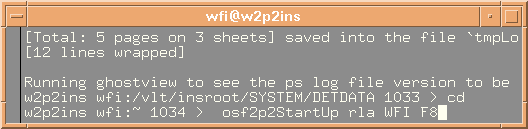
\includegraphics[width=0.45\linewidth]{wfi/wfireboot-0.png}\label{fig:wfisu-launch}
}%
\hspace{0.15\linewidth}
\subfigure[Choose full startup.]{
  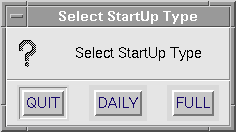
\includegraphics[width=0.2\linewidth]{wfi/wfireboot-1.png}\label{fig:wfisu-full}
}%

\subfigure[Click start.]{
  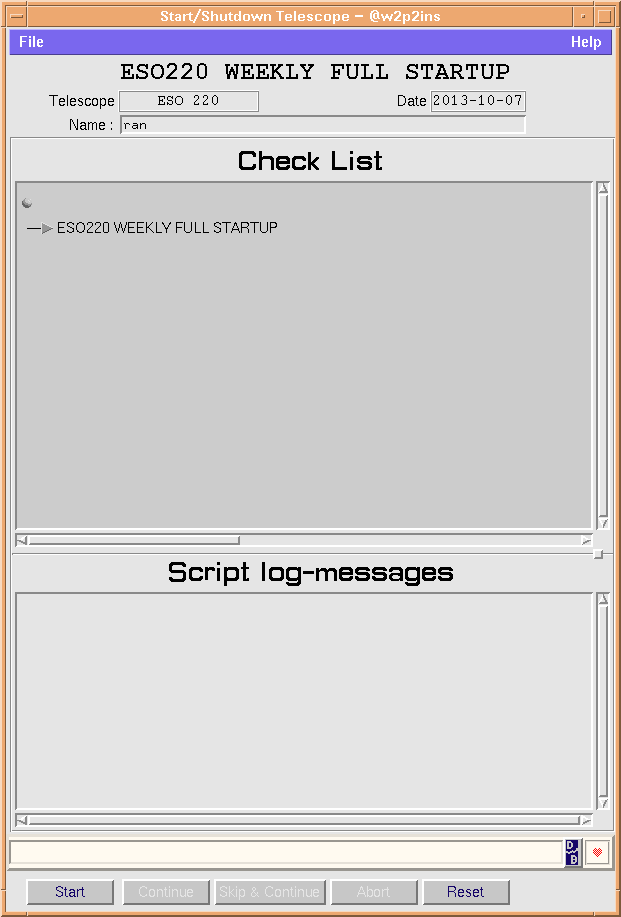
\includegraphics[width=0.365\linewidth]{wfi/wfireboot-2.png}\label{fig:wfisu-start}
  \label{fig:wfi-full-restart}
}%
\hspace{0.05\linewidth}
\subfigure[A log terminal opens. Process takes $\approx $ 10 min.]{
  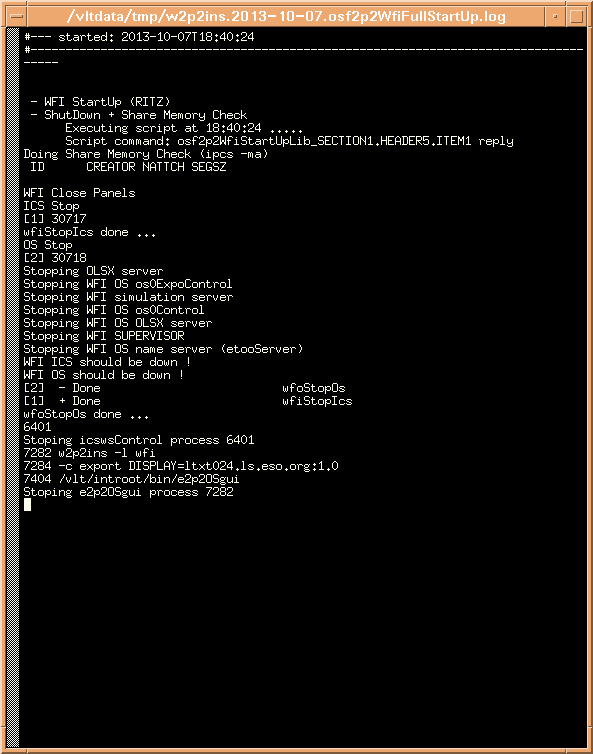
\includegraphics[width=0.42\linewidth]{wfi/wfireboot-3.png}\label{fig:wfisu-log}%
}

\subfigure[When finished select \texttt{File} $\rightarrow$ \texttt{Quit} from
window of Fig.~\ref{fig:wfi-full-restart}. This PDF log opens. You can close 
it.]{
  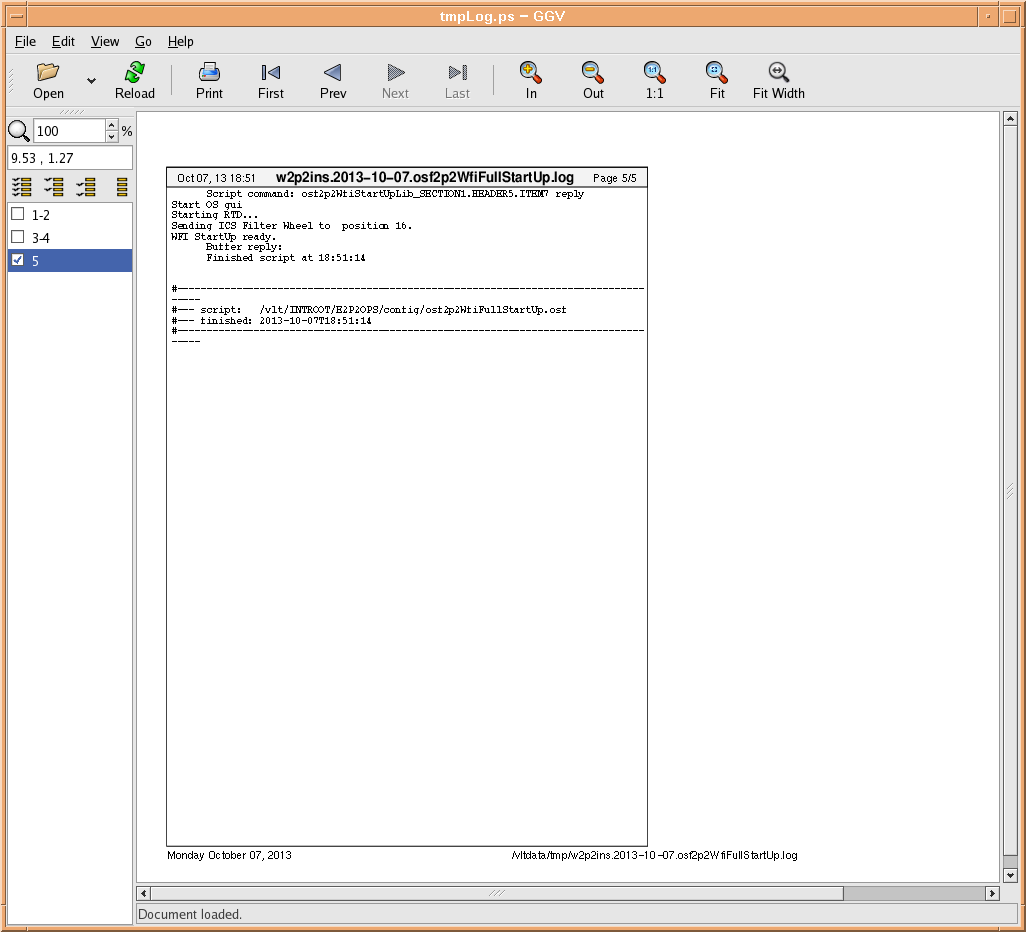
\includegraphics[width=0.41\linewidth]{wfi/wfireboot-4.png}\label{fig:wfisu-pdf}%
}
\hspace{0.05\linewidth}
\subfigure[
Don't forget to rearrange all these windows.  
]{
  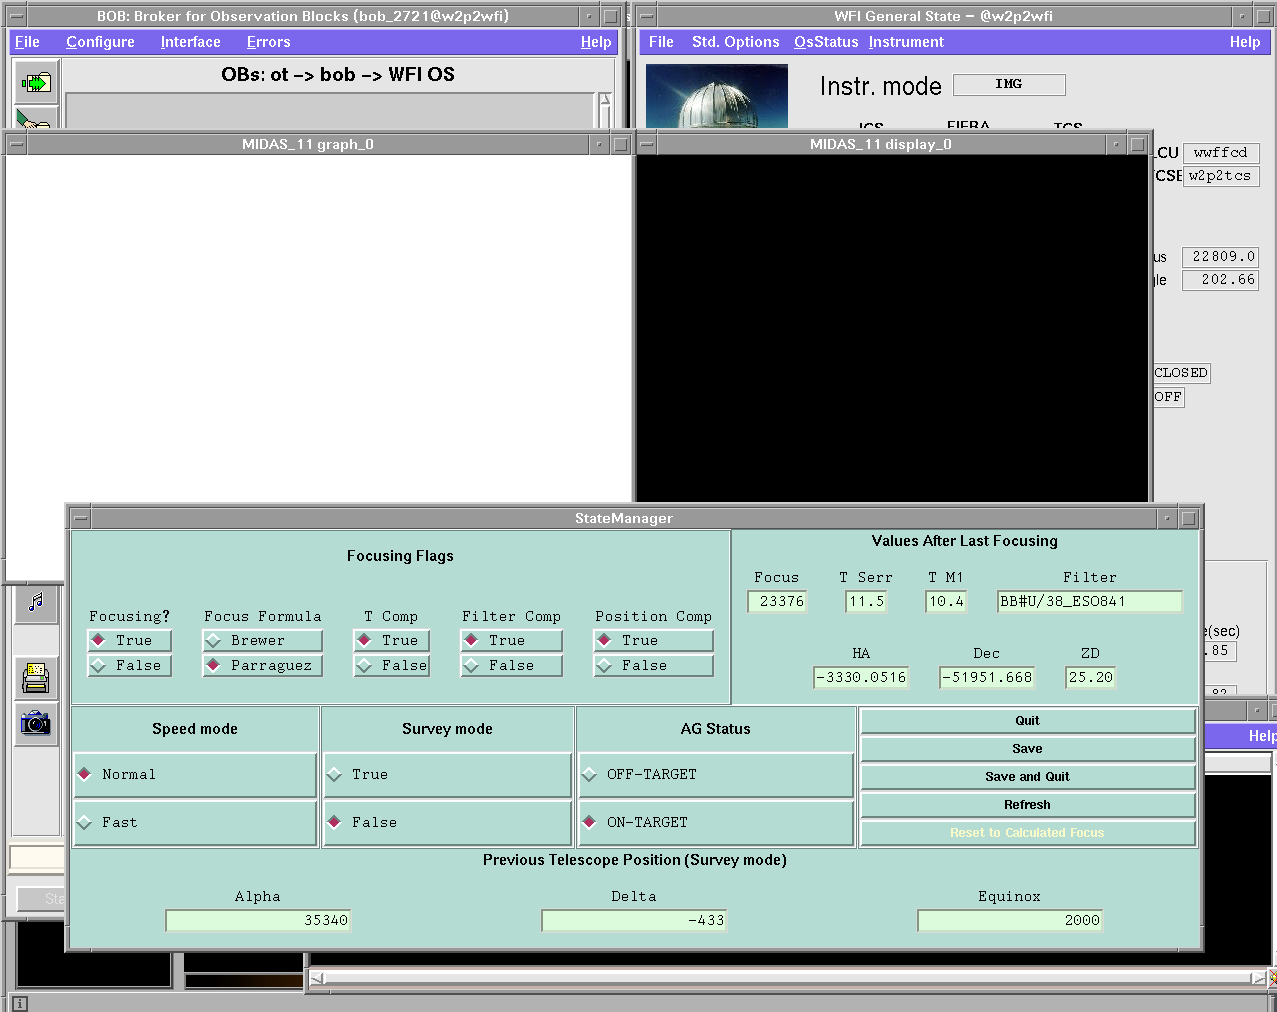
\includegraphics[width=0.47\linewidth]{wfi/wfireboot-5.png}\label{fig:wfisu-windows}%
}
\caption[Wide field imager restart]{\gls{wfi} restart.  When done, don't forget to take a test bias.}
\label{fig:wfi-restart}
\end{figure}

\newpage
\section{TCS startup}

\begin{figure}[h!]
%%
\begin{minipage}{0.4\linewidth}
\centering
\subfigure[Turn hydraulics and drives on, \gls{windows}.]{%
\hspace{0.1\linewidth}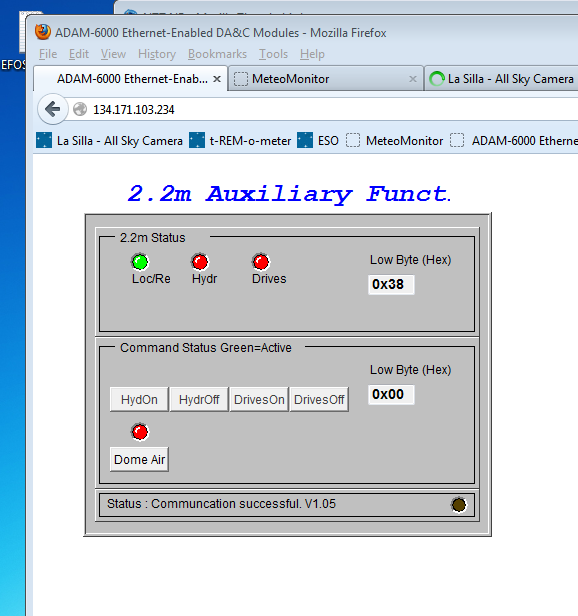
\includegraphics[width=0.8\linewidth]{dome/dome-auxfunc.png}\label{fig:tcssu-hydr}\hspace{0.1\linewidth}%
}
\end{minipage}
%%
\hspace{0.15\linewidth}%%
%%
\begin{minipage}{0.42\linewidth}
\subfigure[On the TCS machine, give \texttt{OK} to this error.]{%
\hspace{0.2\linewidth}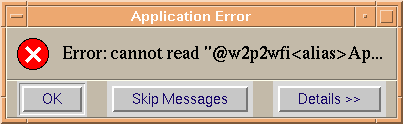
\includegraphics[width=0.6\linewidth]{tcs/tcsreboot-initerror.png}\label{fig:tcssu-error}\hspace{0.2\linewidth}%
}
\subfigure[Reboot lte2p2 machine.]{%
\hspace{0.1\linewidth}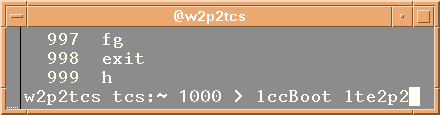
\includegraphics[width=0.8\linewidth]{tcs/tcsreboot-lccboot.png}\label{fig:tcssu-boot}\hspace{0.1\linewidth}%
}
\subfigure[Launch the reboot from the terminal.]{%
\hspace{0.1\linewidth}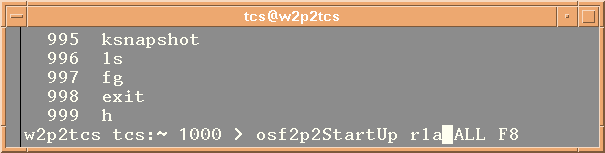
\includegraphics[width=0.8\linewidth]{tcs/tcsreboot-0.png}\hspace{0.1\linewidth}\label{fig:tcssu-launch}%
}
\end{minipage}
\begin{minipage}{0.36\linewidth}
\subfigure[Click start.]{%
  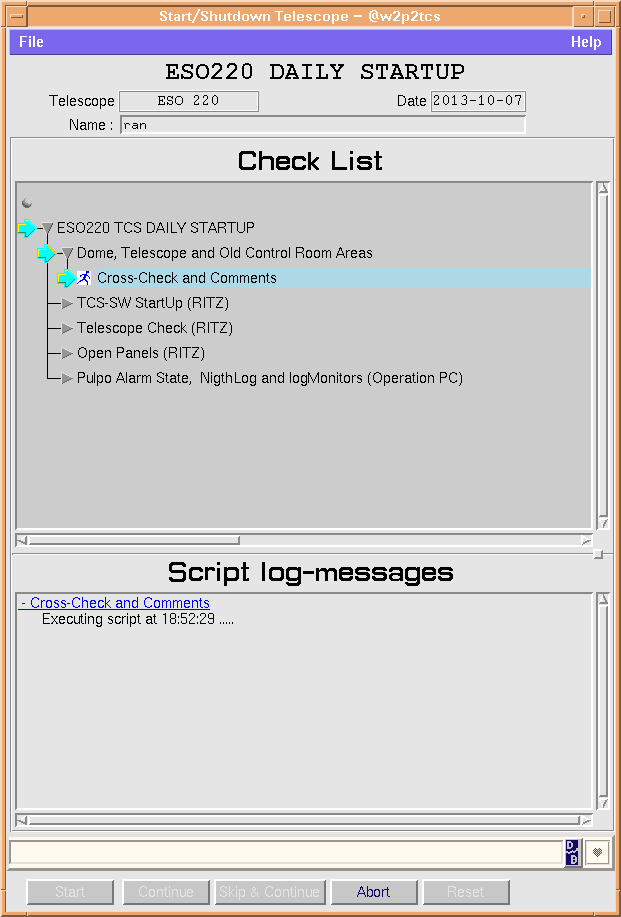
\includegraphics[width=\linewidth]{tcs/tcsreboot-1.png}\label{fig:tcssu-start}%
}%
\end{minipage}
%%%
\hspace{0.14\linewidth}%
\begin{minipage}{0.45\linewidth}
\subfigure[Check elements then click \texttt{OK} to incoming pop-up.]{%
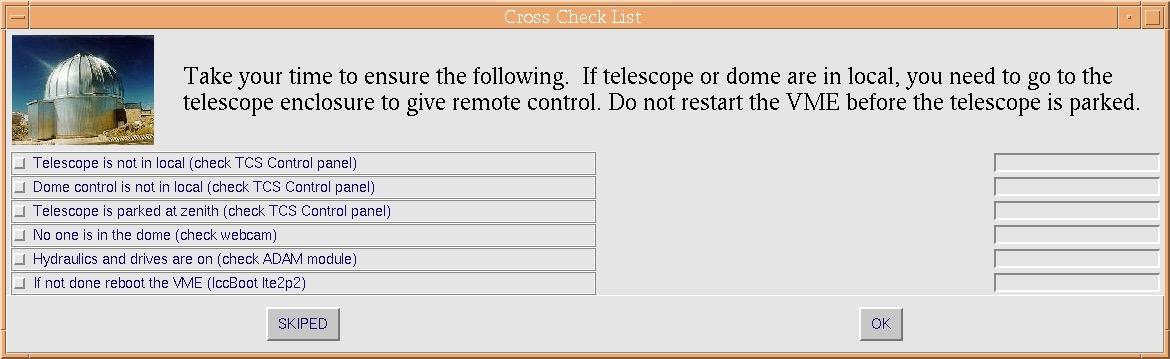
\includegraphics[width=\linewidth]{tcs/tcsreboot-2.jpg}\label{fig:tcssu-check}%
}
\subfigure[Check flat lamp is on or switch it on. 
After clicking \texttt{OK}, telescope should move.]{
  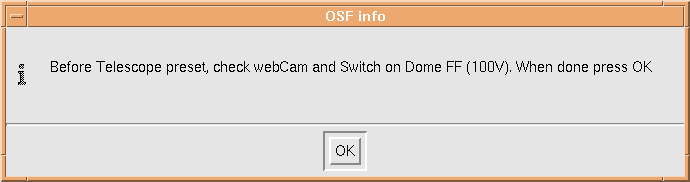
\includegraphics[width=\linewidth]{tcs/tcsreboot-5.png}\label{fig:tcssu-lampon}%
}
\subfigure[Check that CCD alarms are on in the black text window.]{%
\hspace{0.15\linewidth}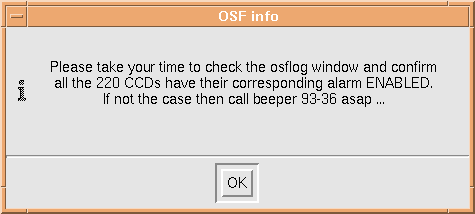
\includegraphics[width=0.7\linewidth]{tcs/tcsreboot-6.png}\hspace{0.15\linewidth}\label{fig:tcssu-alarm}%
}
\end{minipage}
%%%
\begin{minipage}{0.4\linewidth}
\subfigure[Check flat field lamp is off, if not, turn it off]{%
\hspace{0.2\linewidth}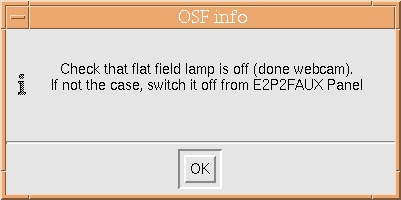
\includegraphics[width=0.6\linewidth]{tcs/tcsreboot-7.jpg}\hspace{0.2\linewidth}%
}%
\end{minipage}
\caption[Telescope control software restart]{\acrshort{tcs} restart. As for \acrshort{wfi} there is a black terminal log) and process ends with a PDF log being popped up.  Emergent windows hould be rearranged to their respective desktops.  The \acrshort{rtd}  isplay should go to all desktops on the left screen, the other windows n the right screen.}
\label{fig:tcs-restart}
\end{figure}
%%%%
%%%% FEROS
%%%%
\newpage
\section{FEROS startup}

\begin{figure}[b!]
\null\hfill
\subfigure[Restart \gls{feros} from terminal. Ensure that telescope
is enabled in the FEROS control window.]{%
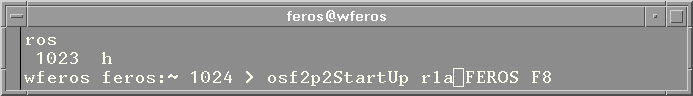
\includegraphics[width=0.62\linewidth]{feros/ferosreboot-0.png}\label{fig:feosu-launch}%
}\hfill
\subfigure[Click \texttt{FULL}.]{%
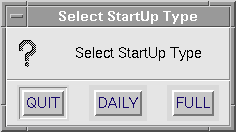
\includegraphics[width=0.18\linewidth]{feros/ferosreboot-1.png}\label{fig:feosu-full}%
}\hfill\null\\
\null\hfill
\subfigure[Click \texttt{START}.]{%
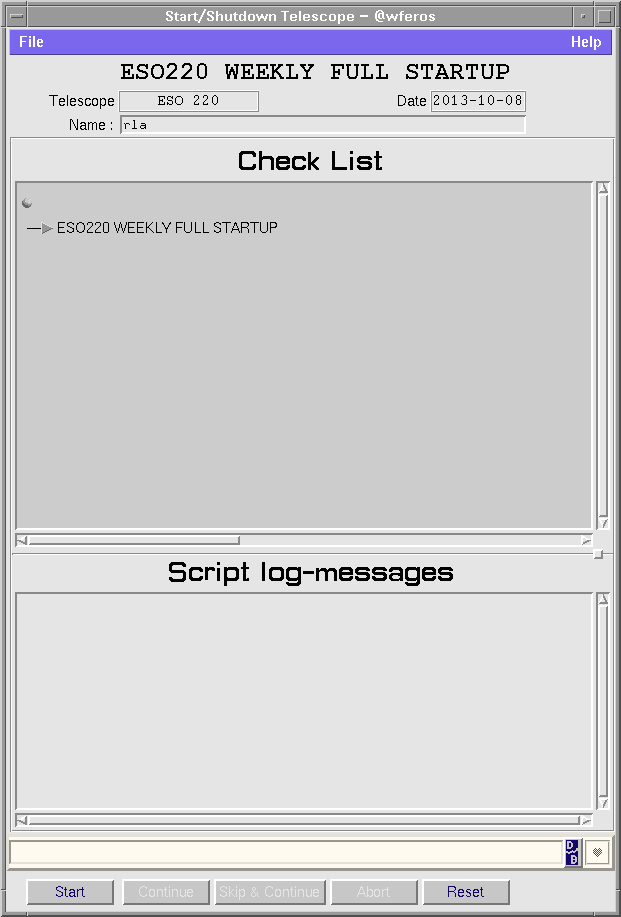
\includegraphics[width=0.35\linewidth]{feros/ferosreboot-2.png}\label{fig:feosu-start}%
}\hfill
\subfigure[This black log opens. Later on a PDF will pop-up.]{%
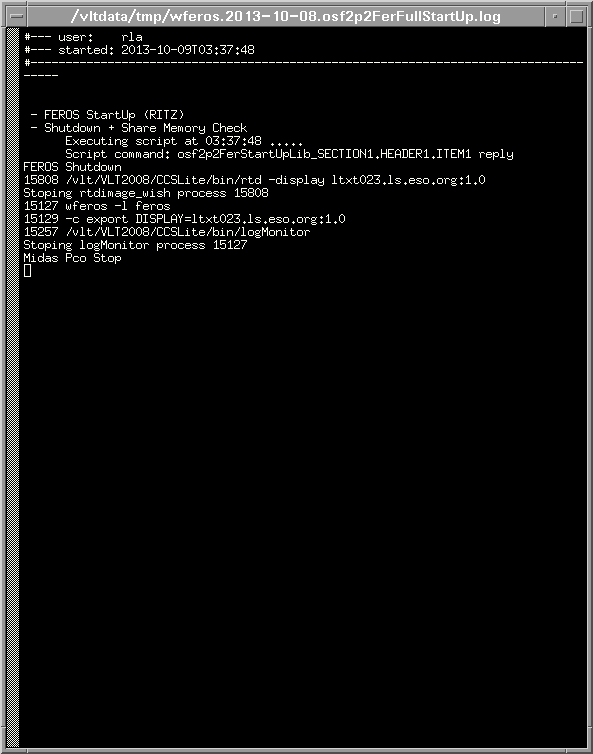
\includegraphics[width=0.40\linewidth]{feros/ferosreboot-3.png}\label{fig:feosu-log}%
}\hfill\null\\
\null\hfill
\subfigure[Click \texttt{START}.]{
  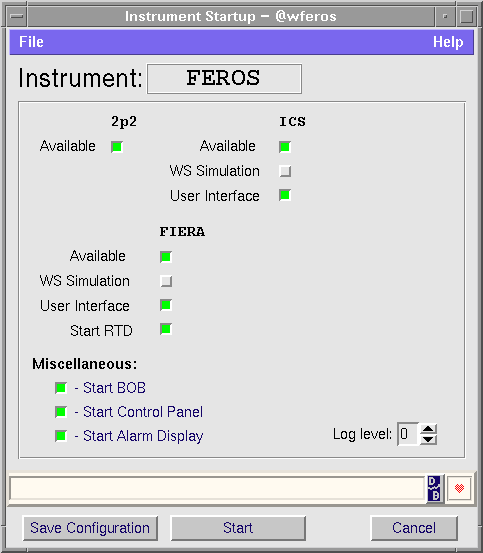
\includegraphics[width=0.31\linewidth]{feros/ferosreboot-4.png}\label{fig:feosu-start2}%
}\hfill
\subfigure[When finished, rearrange the windows to their corresponding
desktops.  \gls{rtd}, \gls{bob} and FEROS control go to \texttt{BOB+OS}.]{
  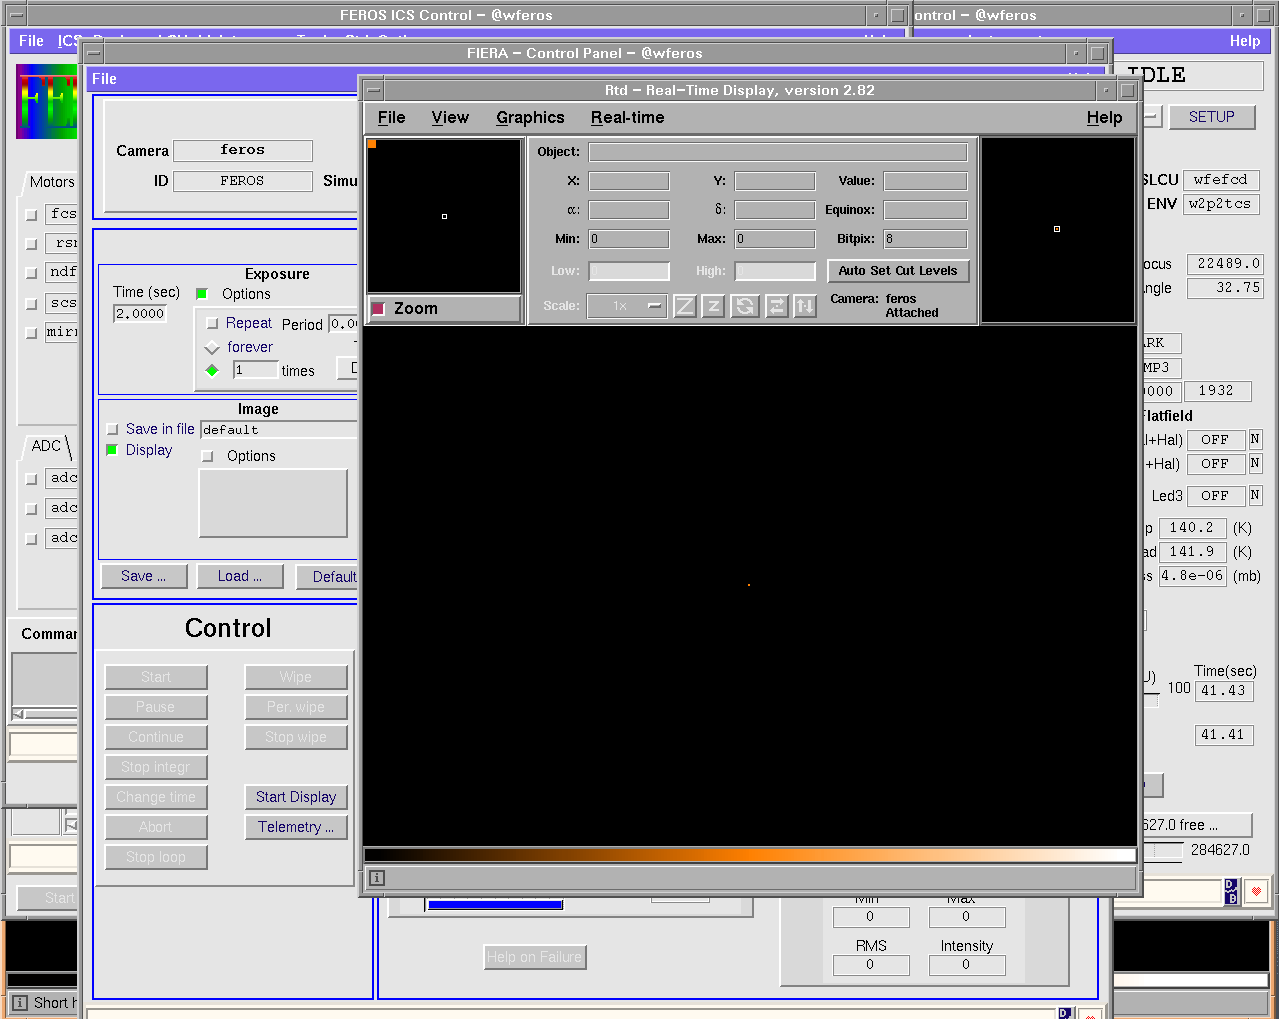
\includegraphics[width=0.45\linewidth]{feros/ferosreboot-5.png}\label{fig:feosu-windows}%
}\hfill\null
\caption{\gls{feros} restart.}
\label{fig:feros-restart}
\end{figure}

\newpage
\section{GROND and FEROS AG}
\begin{figure}[ht!]
\centering
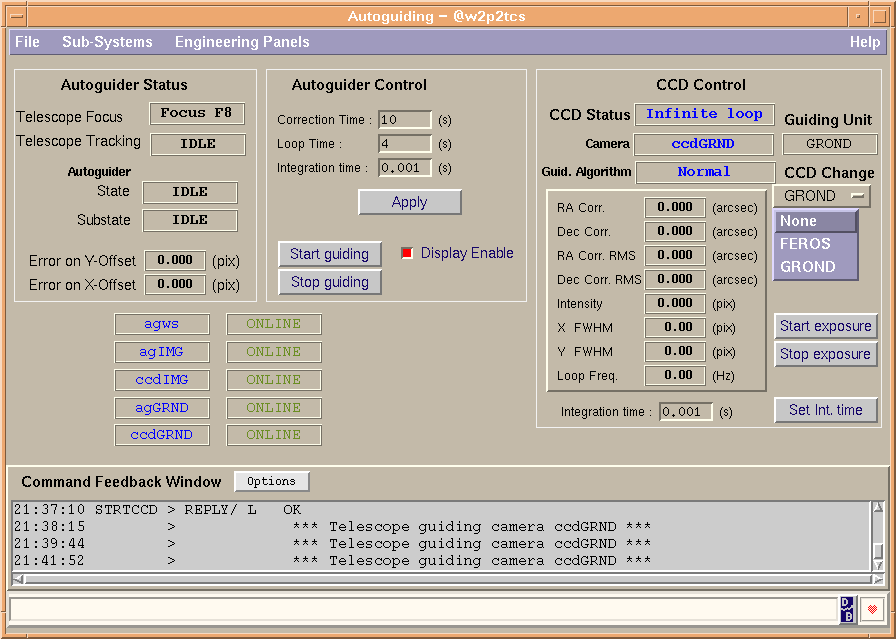
\includegraphics[width=0.7\linewidth]{ag/ag-changecam.png}
\caption[Switching between GROND and FEROS guide cameras]{Switching between \gls{grond} and \gls{feros} guide camera.}
\label{fig:agswitch}
\end{figure}
Check that the \gls{grond} and \gls{feros} guide cameras work by
switching between them on the \gls{ag} window (see Fig.~\ref{fig:agswitch}).
The switching should set the camera in CCD status \texttt{Infinite loop}.  It 
may be necessary to click on \texttt{Start exposure} after switching to
obtain this status.  If status is \texttt{Fail}, the camera must be restarted (see 
Sect.~\ref{sec:agfail}).

%\newpage
\section{FEROS DRS}
\begin{figure}[ht!]
\centering
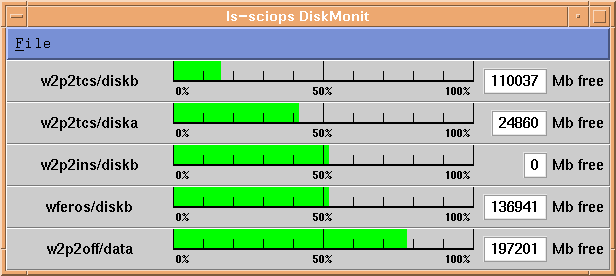
\includegraphics[width=0.3\linewidth]{drs/DiskMonit.png}
\caption{\gls{feros} \gls{drs} Disk Monitor to check free disk space.}
\label{fig:diskmonit}
\end{figure}
%Check \gls{feros} \gls{drs} free disk space.  

\begin{figure}[ht!]
\centering
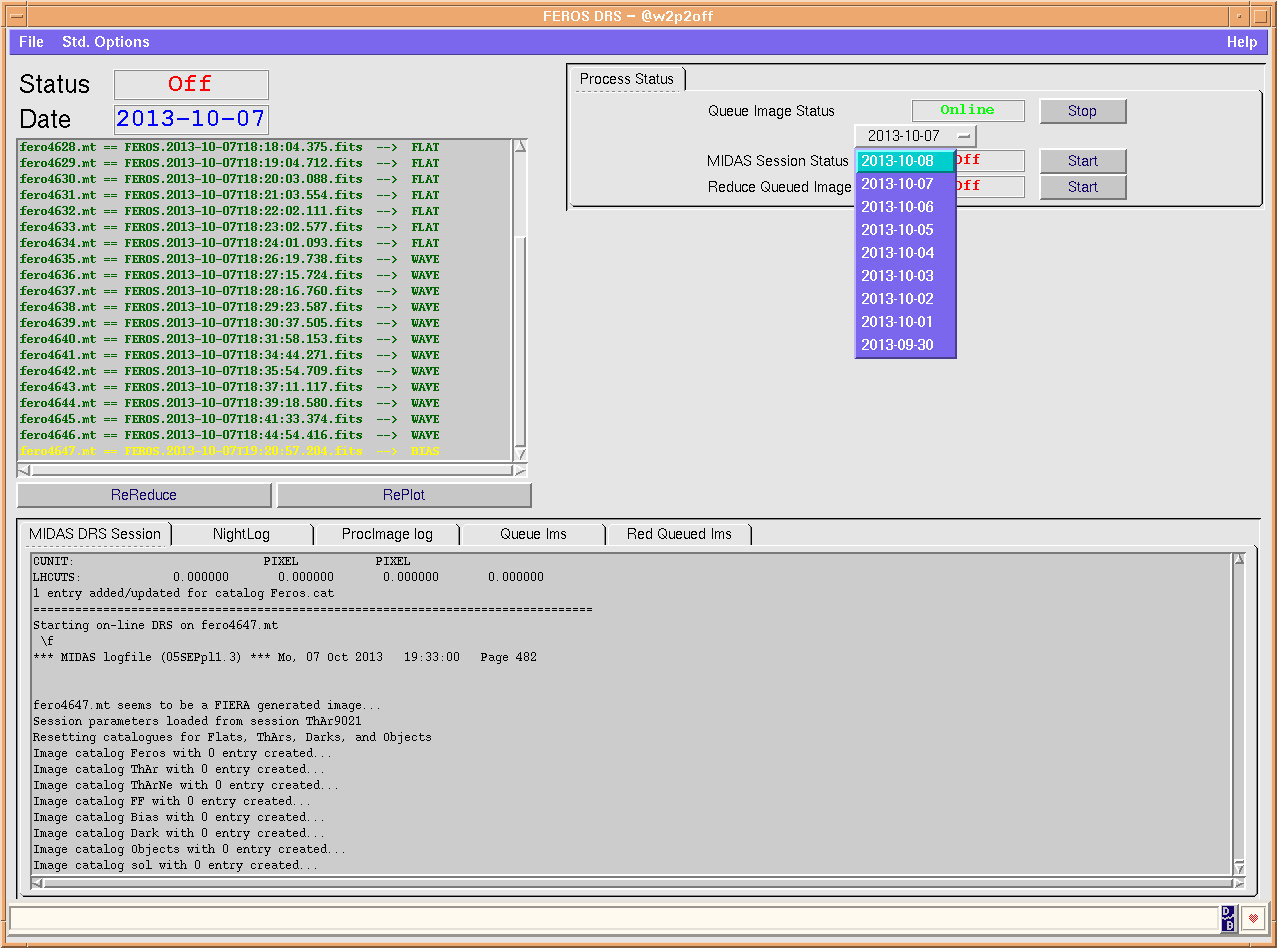
\includegraphics[width=0.45\linewidth]{drs/drs-changedate.png}
\caption{Changing the date of the \gls{feros} \gls{drs}.}
\label{fig:drsswitch}
\end{figure}
The \gls{feros} \gls{drs} should be set to process the data of the 
current night.  In the process the MIDAS session (with its characteristic
blue window) is closed and reopened.  

\section{Additional material}
\subsection{Harmless error messages}
\begin{figure}[ht!]
\centering
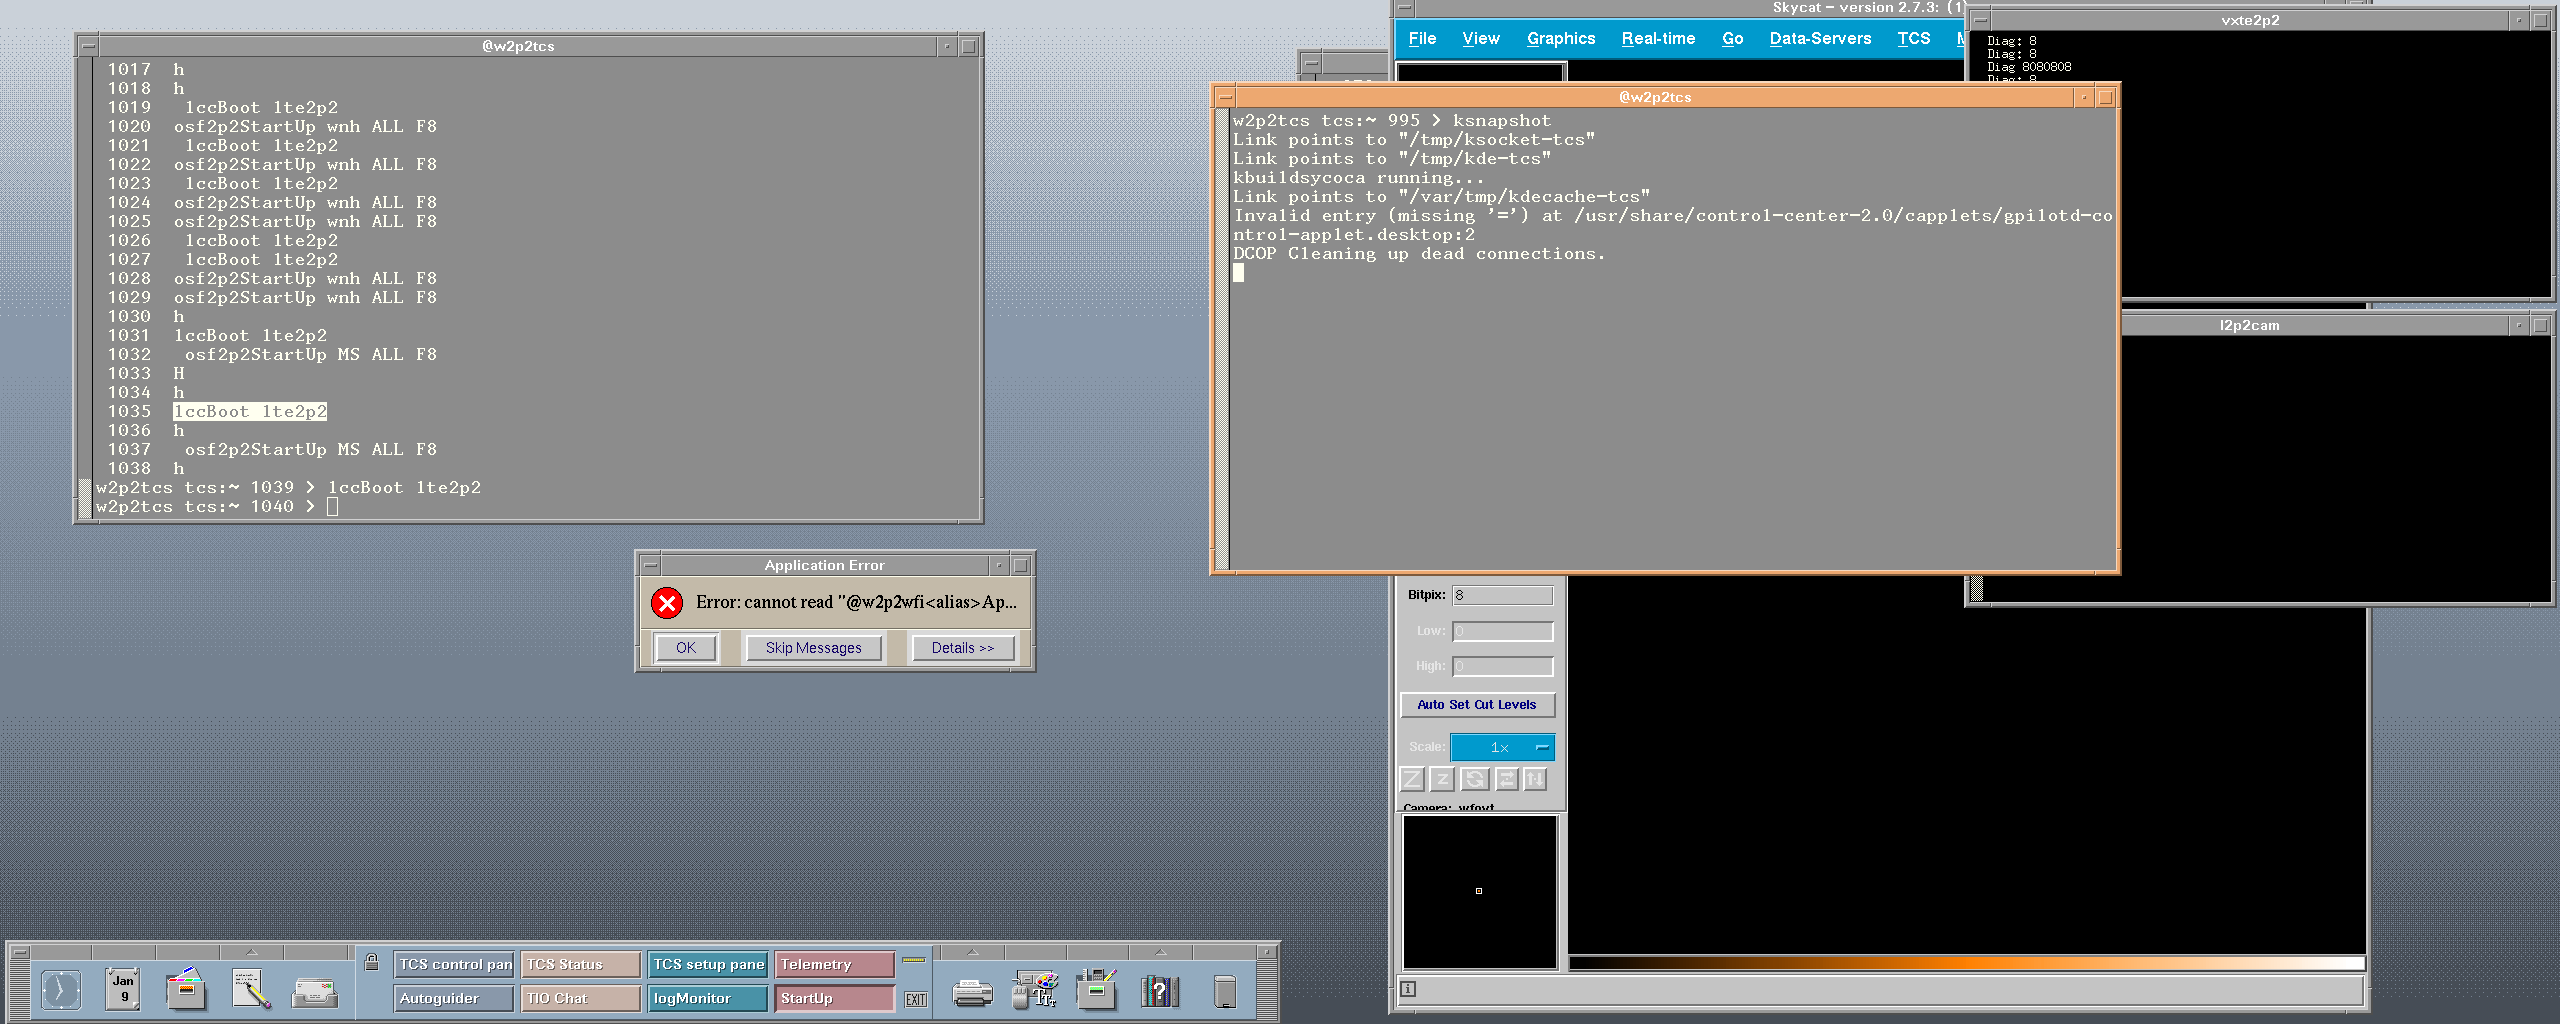
\includegraphics[width=\linewidth]{tcs/tcs-wfi-connection-error.png}
\caption[Harmless error message of the TCS during WFI restart]{When restarting \gls{wfi}, the \gls{tcs} generally issues a harmless
error message.  Get over it and click \texttt{OK}.}
\label{fig:wfistarterror}
\end{figure}

\begin{figure}[ht!]
\centering
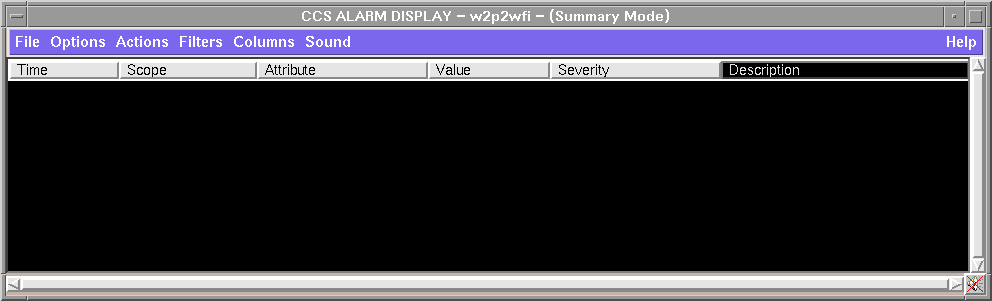
\includegraphics[width=.6\linewidth]{wfi/wfi-ccs-alarm.png}
\caption[Harmless alarm display on WFI during TCS restart]{\texttt{CSS ALARM DISPLAY} will typically pop-up on the \gls{wfi}
screen with a line in red when the \gls{tcs} is restarted.  Get over it and
hide the window.}
\label{fig:wfialarm}
\end{figure}

\subsection{Display settings}
\begin{figure}[ht!]
\null\hfil
\subfigure[Optical]{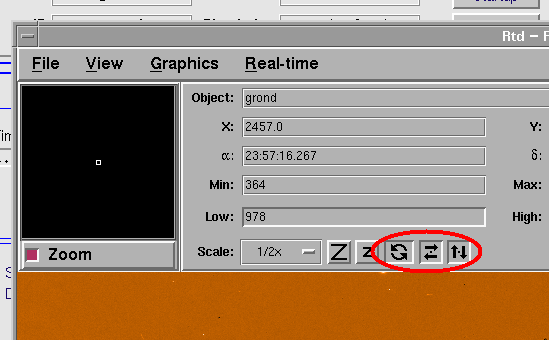
\includegraphics[width=0.60\linewidth]{grond/grond-rtd-flips.png}\label{fig:flip}}%
\hfil
\subfigure[Infrared]{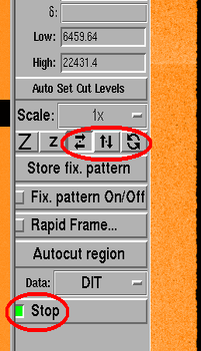
\includegraphics[width=0.20\linewidth]{grond/grond-irtd-flips.png}\label{fig:iflip}}
\hfil\null
\caption[Correct sky orientation of the GROND displays]{Correct sky orientation of the \gls{grond} displays. The infrared one
is receiving data in real time (green checkbox).}
\end{figure}

%%%%%%%%%%%%%%%%%%%%%%%%%%%%%%%%%%%%%%%%%%%%%%%%%%%%%%%%%%%%%%%%%%%%%%%%%%%



\chapter{Afternoon: Day-time calibrations}
\label{daycal}

The day-time observations use \glspl{ob} either stored in \gls{bob} or in a
\gls{ot} queue.  Managing \glspl{ob} with \gls{bob} and \gls{ot} is
explained in more detail in Sect.~\ref{ob}.

\section{WFI}
Internal calibrations and health checks are typically left running in the morning after the dome has been closed.  See Sect.~\ref{sec:clocal}.

\procedure{WFI dome flat-fields}
   \begin{enumerate}
     \item Ensure that no one is in the dome nor will enter it.
     \item Prepare the telescope.
         \begin{enumerate}
            \item If hydraulics is off, switch it on and wait for connection with VME
                \begin{enumerate}
                    \item On the \texttt{Dome Auxiliary Functions} panel click \texttt{Hydr On} then \texttt{Drives On}.
                    \item On the \texttt{Telscope Control} panel, check if red message appears  \texttt{no connection}.
                    \item If it is the case, wait for it to disappear (about 2 min)
                \end{enumerate}
            \item If hydraulics were off, initialise telescope
                \begin{enumerate}
                    \item On the \texttt{Telescope Setup} panel, click \texttt{Tel Init}
                    \item Wait for the telescope status of  the \texttt{Telescope Control} to go from \texttt{WaitIni} to \texttt{Slew} (2 min)
                \end{enumerate}
            \item Preset to flat-field screen
            \begin{enumerate}
                \item Go to the \texttt{TCS Setup Panel} (Fig.~\ref{fig:tcssetup}) on screen \texttt{Telescope Control Software}.
                \item Put \texttt{Dome} on \texttt{automatic}.
                \item Preset the telescope to flat-field screen.\\
                  Click \texttt{FF Scr} below \texttt{Fixed Presets}
                \item Wait for the movement to complete (2 min) before starting the flat-field \gls{ob}.\\
                  On the \texttt{TCS Control Panel} (Fig.~\ref{fig:tcs}) telescope status is \texttt{Slew}.
            \end{enumerate}
            \item Prepare shutters and mirrors
            \begin{enumerate}
               \item Click \texttt{Open} under the \texttt{Main Mirror Cover}.
               \item Wait for opening to complete (2 min) befor starting the flat-field \gls{ob}
               \item Open the \gls{wfi} protective shutter.\\
                     In the \gls{auxfunc} (Fig.~\ref{fig:tcsauxfunc}), \texttt{OPEN} the \texttt{WFI PROTECTIVE SHUTTER}.
               \item Ensure the GROND mirror is on WFI
               \item Ensure the FEROS mirror is on FEROS
             \end{enumerate}
         \end{enumerate}
     \item Prepare the flat-field \gls{ob}
     \begin{enumerate}
        \item Go to \gls{bob} on the screen \texttt{BOB Wide Field Imager}.
        \item Fetch \gls{bob} from file (\fetchob) looking in subfolder \texttt{DomeFlats}.
        \begin{itemize}
           \item If observing in UBVRI standard filtres: \texttt{DomeFlatCalPlan\_new.obd} (25 min).
           \item During an observing period or a visitor run, a custom OB may be used: \texttt{DomeFlatsP102.obd} or         \texttt{DomeFlatsVisitorName.obd}
           \item To choose filtres on the fly: \texttt{DomeFlatGeneric\_new.obd}.
           \item To test all filtres: \texttt{DomeFlatAllSnapshot.obd} (1 flat per filtre, 2 hrs 30 min).
        \end{itemize}
        \item If choosing filtres on the fly, customise the ob
              \begin{enumerate}
                 \item Open the flat template, left-clicking on the triangle of \texttt{WFI\_img\_cal\_DomeFlat\_new}
                 \item Open the instrument section, left-click on the triangle of section \texttt{INS}
                 \item Use \wmenu{Interface}{Engineering}.
                 \item Middle-click the filtre name, fill in value, and type enter.\\
                       Name is \texttt{ESONNN\_name/width} (\texttt{NNN}: number, \texttt{name}: filtre name or wavelength)\\
                       In virtual desktop \texttt{WFI ICS}, a filtre list is found below \texttt{SETUP Instrument}
                 \item Deactivate the filtres you don't want.\\
                       Right-click the triangles to get a thumb down
              \end{enumerate}       
     \end{enumerate}
     \item Execute \gls{ob} (15--30 min usually).
     \item If no other types of flats are done, park the telescope 
     \begin{enumerate}
         \item Go to the \texttt{TCS Setup Panel} on screen \texttt{Telescope Control Software}.
         \item \texttt{Close} to the \texttt{Main Mirror Cover}.
         \item Set the dome in \texttt{Manual}.
         \item Click \texttt{Zenith} below \texttt{Fixed Presets} (2 min)
         \item Close the \gls{wfi} protective shutter.
           In the \gls{auxfunc} (Fig.~\ref{fig:tcsauxfunc}), \texttt{CLOSE} the \texttt{WFI PROTECTIVE SHUTTER}.
     \end{enumerate}
     \item If telescope will stay idle for hours, switch hydraulics off.
   \end{enumerate}



\section{FEROS}

A linearity check is left running in the morning (see Sect.~\ref{sec:clocal}). The standard \gls{feros} calibration is generally done after startup.  It is internal in a separate room, so it can be done while doing telescope movements, going to the dome, or even \gls{wfi} or \gls{feros} observations.

\procedure{FEROS afternoon calibrations}
\begin{enumerate}
  \item Go to screen \texttt{FEROS BOB}.
  \item Check that FEROS does not communicate with the telescope\\
        On the \texttt{FEROS General State} panel, use \wmenu{Telescope}{Ignore}.
  \item Execute \texttt{StanCalNorm.obd} from \gls{bob} ($\approx 1$\,h).
    \begin{enumerate}
       \item Use \fetchob.
       \item Click \texttt{Start}.
    \end{enumerate}
  \item Check that the \gls{drs} has processed it.  \textbf{While Fabry-Pérot stays installed, it will fail.}
    \begin{enumerate}
      \item Find a white graphics with title \texttt{OBJ FIB GUESS}.
      \item The wavelength solution should have $4 \times 10^{-3}$ Angstroem
         rms or less and look flat.
      \item If not, restart calibration if possible.
    \end{enumerate}
\end{enumerate}

\section{GROND}

GROND calibrations are left running in the morning after the dome has been closed (see Sect.~\ref{sec:clocal}). Some observers may ask for GROND linearity calibration using dome flats, providing the observing blocks and a detailed explanation.


%%%%%%%%%%%%%%%%%%%%%%%%%%%%%%%%%%%%%%%%%%%%%%%%%%%%%%%%%%%%%%%%%%%%%%%%%%

\chapter{Sunset: Getting ready}
\label{sec:sunset}

\section{Opening}
\label{sec:open}

Opening should take place about one or two hours before sunset if conditions allow it. In case of doubts, always ask to the day-time Telescope \& Instrument Operator of ESO.

\procedure{Dome opening and telescope readying}
\label{list:open}
\begin{enumerate}
\item Check that the slit is oriented opposite to the Sun. It does not apply when opening at night.
        \begin{enumerate}
            \item On the \texttt{rose diagram} of the \texttt{TCS Control Panel}, it should be to the East
            \item If not, rotate manually in the \texttt{TCS Setup Panel}
        \end{enumerate}
\item Open the slit\label{list:slitopen}
         \begin{enumerate}
           \item Go to the \gls{tcs} setup panel (Fig.~\ref{fig:tcssetup})
           \item Check that the value below \texttt{Main Mirror Cover} is \texttt{closed}.
           \item If not, click \texttt{Close} (2 min).
           \item n the \gls{tcs} setup panel (Fig~\ref{fig:tcssetup}), below \texttt{slit}, click \texttt{Open} (1 min)
         \end{enumerate} 
\item Turn on the Dome Air in the \gls{domefunc} (\gls{windows}, Fig.~\ref{fig:domefunc}).
\item If opening during the night, you can directly prepare the telescope (Procedure~\ref{proc:ready}).
\end{enumerate}

\section{Telescope readying}

A bit before sunset if doing sky flats or at sunset otherwise, you can ready the telescope and point to an empty field.

\procedure{Telescope readying}\label{proc:ready}
\begin{enumerate}
\item Prepare the telescope
         \begin{enumerate}
            \item If hydraulics is off, switch it on and wait for connection with VME
                \begin{enumerate}
                    \item On the \texttt{Dome Auxiliary Functions} panel click \texttt{Hydr On} then \texttt{Drives On}.
                    \item On the \texttt{Telscope Control} panel, check if red message appears  \texttt{no connection}.
                    \item If it is the case, wait for it to disappear (about 2 min)
                \end{enumerate}
            \item If hydraulics were off, initialise telescope
                \begin{enumerate}
                    \item On the \texttt{Telescope Setup} panel, click \texttt{Tel Init}
                    \item Wait for the telescope status of  the \texttt{Telescope Control} to go from \texttt{WaitIni} to \texttt{Slew} (2 min)
                \end{enumerate}
	\item\label{list:mirropen}Open the main mirror cover
            \begin{enumerate}
               \item Click \texttt{Open} under the \texttt{Main Mirror Cover}.
               \item Wait for opening to complete (2 min) befor starting the flat-field \gls{ob}
            \end{enumerate}
        \end{enumerate}
        \item Preset to an empty field if doing sky flats, a test with GROND, or readying before sunset
               \label{list:presetempty}         
            \begin{enumerate}
            \item Go to the \gls{tcs} Control Panel (Fig.~\ref{fig:tcs}) 
            \item Below \texttt{Catalogue Handling} click \texttt{Cat. Select}.
            \item Choose \texttt{Empty Fields 2011}
            \item Select field with \texttt{Up} and \texttt{Dwn}.\\
                  Right ascension should be about 1 hour more than sidereal time at sunset.\\
                  Consider field quality: excellent, good, OK, poor.
            \item Click \texttt{Preset}.
            \end{enumerate}      
         \item Set the dome motion in automatic.\label{list:domeauto}\\
               On the \gls{tcs} setup panel (Fig~\ref{fig:tcssetup}), below \texttt{Dome}, select the checkbox \texttt{Automatic}.
\end{enumerate}


\section{Making the instruments ready (at sunset)}
\label{sec:insprep}

\procedure{Making instrument ready}
\begin{enumerate}
   \item Activate the connection between instruments and telescopes
       \begin{enumerate}
         \item On the \gls{feros} control panel (Fig.~\ref{fig:feroscon}), use \wmenu{Telescope}{Enable}.
         \item On the \gls{grond} control panel (Fig.~\ref{fig:grondcon}), click \texttt{TCS ON}.
         \item Refresh the \gls{wfi} general state panel (Fig.~\ref{fig:wfigen}).
               \begin{itemize}
                 \item Use \wmenu{Std. Options}{Refresh Database values}.
                 \item Check that \texttt{TCS} is \texttt{ONLINE}.
               \end{itemize}
       \end{enumerate}
  \item  Open the instrument covers
    \label{list:opencov}
     \begin{enumerate}
        \item In the \gls{auxfunc} (Fig.~\ref{fig:tcsauxfunc}), open the 
              \gls{wfi} protective shutter.
        \item For \gls{grond} observations, in a terminal open the main cover, the cold shutter, and the optical ones through these commands
            \begin{enumerate}
              \item \texttt{grondMC OPEN}
              \item \texttt{grondCS OPEN}
              \item \texttt{grondSHUTTER}
            \end{enumerate}
     \end{enumerate}
  \item Check for mirrors
     \label{list:checkmirror}
     \begin{enumerate}
        \item Check \gls{feros} mirror (\texttt{M3 Selected Mirror}) on the \gls{feros} control panel (Fig.~\ref{fig:feroscon}).\\
              If necessary, set \texttt{mirr3} motor on the \gls{ics} (Fig.~\ref{fig:ferosics})
              \begin{itemize}
                \item to \texttt{WFI} for observations with \gls{wfi} or \gls{grond};
                \item to \texttt{FEROS} for observations with \gls{feros}.
              \end{itemize}
              (Select the \texttt{mirr3} check box, select instrument, click \texttt{SETUP}, unselect checkbox.)
        \item Check \gls{grond} mirror on the \gls{grond} control (Fig~\ref{fig:grondcon}).\\
              If necessary, type 
              \begin{itemize}
                  \item \texttt{grondM3 WFI} for \gls{feros} or \gls{wfi} observations
                  \item \texttt{grondM3 GROND} for \gls{grond} observations.
              \end{itemize}
     \end{enumerate}
  \item If no test OB with TCS on was done during the start-up, try to run a \gls{grond} test OB (\texttt{1min1TD\_test.obd}) on sky using \gls{bob} (Fig.~\ref{fig:grondbob}).
     \begin{enumerate}
       \item Fetch \gls{ob} with \fetchob.
       \item Click \texttt{Start}.      
       \item If an error occurs after the optical exposure has started
             \begin{itemize}
                \item Click \texttt{OK} on the error popups
                \item Wait for the exposure to finish
                \item In \gls{bob}, click on \texttt{Reset status}
                \item Click on start again.
                \item If error persists, close \gls{bob} and open it again
             \end{itemize} 
       \item For other errors, do a \texttt{grondSHUTTER}, close bob and open it again.
     \end{enumerate}
\end{enumerate}

\section{Refining the night plan}

On the GROND remote observer screen at the side of the small laptop, one of the GROND team members should have contacted you by \texttt{slack} to indicate their observing plan, if they have some monitoring to do.  It generally consists of 1--3 targets to be observed within a time range, so that you try to accommodate with your own and/or other service observations.  If it is detrimental to the other observations, there is sometimes some flexibility on which days they have their monitoring done, ask, but they have precedence.

If slack is closed, open a browser with the following link: https://slack.com/signin. Sign in to workspace grondobs.slack.com and continue. Use the credentials given on the cover of the laptop, account \texttt{lasillaskype} with password \texttt{pwd}$\star\star\star\star\star$. Under channel \texttt{remote\_observing} you can usually find the observing plan (late afternoon). 


%-------------------------------------------------------

\chapter{Twilight: On-sky calibrations}
\label{nightcal}


\section{Outline}

\paragraph{Flat-fielding}
\begin{enumerate}
  \item \gls{wfi} flats can be done from sunset to sun at $-10$ degrees elevations depending on filtre.\\
        Standard filtres have that order: U, V, R, I, and B.
  \item \gls{grond} flats are extensive and run from sun at $-4$ to $-9$ degrees elevation.\\
        To be started when 2s J-band exposures feature a
        relatively flat field with 20\,000 counts.
\end{enumerate}

\paragraph{Pointing \& Focus}
\begin{enumerate}
  \item Pointing should be performed daily with \gls{wfi}
        using an \gls{ob} from \gls{bob}.
  \item \gls{feros} focus should be performed nightly using an \gls{ob} from
        the \gls{ot} calibration queue.
  \item \gls{wfi} focus should be done closest to science observations.
\end{enumerate} 

\paragraph{Standards}
\begin{enumerate}
  \item \gls{feros} focus includes an optional spectrophotometric standard.
  \item \gls{wfi} \& \gls{grond} standard fields are available from their respective \glspl{bob}.
\end{enumerate}

\section{WFI}


\subsection{Sky flats}
\label{sec:wfiflats}
Sky flats in most narrow-band filtres and the darkest broad-band ones ($U$ \& $V$) should be started right at sunset or slightly before sunrise.  The brightest
broad band filtres ($R$, $I$, $B$) can be obtained with the sun at $-6$ to
$-9$ degrees approximately.  It is possible to obtain the five standard filtres in one twilight provided they are started at sunset or in the morning twilight when the sun is at $-9$ degrees.

The procedure has been somehow modified (January 2014).  

\procedure{Taking sky flats with WFI}
\begin{enumerate}
  \item If not done, check that dome and main mirror cover are open (Sect.~\ref{sec:open}, point~\ref{list:open}). 
  \item If not done, check \gls{grond} and \gls{feros} mirrors (Sect.~\ref{sec:insprep}, point~\ref{list:checkmirror}).
  \item If not done, check that the WFI main cover is open (Sect.~\ref{sec:insprep}, point~\ref{list:opencov}).
  \item If not done, point the telescope to an empty field (Sect.~\ref{sec:open}, point~\ref{list:presetempty}).
      \begin{enumerate}
         \item Go to \texttt{TCS control panel} the on screen \texttt{Telescope Control Software}.
         \item Below \texttt{Catalogue handling} click \texttt{Cat. Select}.
         \item Choose \texttt{Empty Fields 2011}
         \item Select field with \texttt{Up} and \texttt{Dwn}.\\
               Right ascension should be about 1 hour from sidereal time, opposite to the Sun.\\
               Consider field quality: excellent, good, OK, poor.
         \item Click \texttt{Preset}.
      \end{enumerate}
  \item Go to \gls{bob} on screen \texttt{BOB Wide Field Imager}.
  \item Fetch sky flat \gls{ob} from file (\fetchob).\\
        (Go to folder \texttt{.../TEMPLATES/OBD/SkyFlats/})
    \begin{itemize}
       \item For standard filtres use \texttt{SkyFlatsEveningCalPlan.obd}\\
           (\texttt{SkyFlatsMorningCalPlan.obd} in the morning)
       \item Some other filtres have their own flat OBs (e.g. \texttt{SkyFlatsI203}).
       \item For a set of non standard filtres use \texttt{SkyFlatsGeneric.obd}.
    \end{itemize}
  \item If not doing the standard filtres, customise \gls{ob}.
    \begin{enumerate}
       \item For non standard filtres, edit the filtre names.
             \label{list:editfilt} 
              \begin{enumerate}
                 \item Open the flat template, left-clicking on the triangle of \texttt{WFI\_img\_cal\_DomeFlat}
                 \item Open the instrument section, left-click on the triangle of section \texttt{INS}
                 \item Use \wmenu{Inteferface}{Engineering}.
                 \item Middle-click the filtre name, fill in value, and type enter.\\
                      (In virtual desktop \texttt{OS GUI}, a filtre list is found below \texttt{SETUP Instrument})
              \end{enumerate}
       \item Deactivate unneeded templates.\\
             Right-click the triangles to get a thumb down.
    \end{enumerate}
  \item Execute \gls{ob}
    \begin{enumerate}
      \item Click \texttt{Start}.
      \item For each template
       \begin{enumerate}
         \item Click \texttt{OK} to pop-up asking to preset.
         \item After one minute, a pop-up estimates the exposure time.\\
           In the evening, if the message is
           \begin{itemize}
             \item an error message and a dimm test image ($\le 400$\,ADU), skip this template
           \end{itemize}
           In the morning, if the message is
           \begin{itemize}
             \item an error message and a bright test image ($\ge 20$\,kADU), skip this template
           \end{itemize}
       \end{enumerate}
    \end{enumerate}
\end{enumerate}


\subsection{Pointing} 

\subsubsection{Pointing with FEROS}

If starting with FEROS, you can use the focus and/or standard star OB to check pointing.

\procedure{Ensure that pointing is correct using FEROS}
\begin{enumerate}
  \item Update the model parameters
  \begin{enumerate}
     \item Go to the \texttt{Telescope Control Software} workstation.
     \item Open or use a UNIX terminal.
     \item Type  \~{}\texttt{/bin/fixPointing.sh}
  \end{enumerate}
  \item Change pointing model to FEROS.
  \begin{enumerate}
    \item Go to the \texttt{TCS Status Panel} (workspace \texttt{Status}, see Fig.~\ref{fig:tcsstatus}).
    \item Use \wmenu{Instrument selection}{FEROS}
  \end{enumerate}
  \item Check the sidereal time
  \begin{enumerate}
    \item On the digital clock of the control room, switch display to sidereal time.
    \item Go to the \texttt{TCS Control Panel} (workspace \texttt{Control}).
    \item The sidereal time of the TCS Control Panel should lag by approximately 5 s. 
  \end{enumerate}
  \item Point at a FEROS focus/standard star. See Sect.~\ref{sec:ferosfocus}.
\end{enumerate}

\subsubsection{Pointing and autoguider test with WFI}

If things go well, the bright star used for the test that should fall a few hundreds of pixels from the centre of the mozaic in the South-West direction. 

\procedure{WFI pointing}
\begin{enumerate}
  \item Switch the instrument to \gls{wfi} on the \gls{tcs} status panel.\\
    (\texttt{Instrument Selection}, Fig.~\ref{fig:tcsstatus}. Do it even if it already says \gls{wfi}).\label{list:switchwfi}
  \item If not done, check that dome and main mirror are open, and dome is in automatic.\\
    (Refer to Sect.~\ref{sec:open}, points~\ref{list:slitopen}, \ref{list:mirropen} and \ref{list:domeauto}). 
  \item If not done, check \gls{grond} and \gls{feros} mirrors (Sect.~\ref{sec:insprep}, point~\ref{list:checkmirror}).
  \item If not done, check that the WFI main cover is open (Sect.~\ref{sec:insprep}, point~\ref{list:opencov})\label{list:pointing:opencov}.
  \item Go to \gls{bob} on screen \texttt{BOB Wide Field Imager}.
  \item Fetch pointing \gls{ob} from file (\fetchob).\\
        (Go to folder \texttt{.../TEMPLATES/OBD/Pointing/})
        \begin{itemize}
           \item OBs are \texttt{Pointing-<ra>h.obd}, where \texttt{<ra>} is the right ascension.
           \item Chose an OB with \texttt{<ra>} close to sidereal time.
        \end{itemize} 
  \item After the exposure is taken, accept ``refine acquisition''.\\
        A small form asking for the star's coordinates will appear.
  \item Use \texttt{Pick Object} in the \texttt{view} option of the \gls{rtd} to obtain the star's pixel coordinates.  
  \item Input the pixel coordinates.\\
        Copy them with the mouse from the Pick Object popup to the small form. 
  \item \textbf{TEMPORARY: if offset values are large, it's normal, WFI pointing was modified.}
        After \texttt{offset and quit} a popup should have appeared.\\
        Click \texttt{OK} if satisfied with the offset values (in arcsec).
  \item If no star at all is seen, see 
    Sect.~\ref{sec:trouble:pointing} to check that:
    \begin{enumerate}
      \item You did not forget Points \ref{list:switchwfi}-\ref{list:pointing:opencov}.
      \item The sidereal time of the \gls{tcs} is correct within seconds.
      \item The pointing parameters of the \gls{tcs} are correct.
      \item Check that the star does not fall into the gap between two CCDs. (Give coordinates falling in the gap to the pop-up, offset and reaquire. 
      \item Once you have a star, as long as the offset is large, use \texttt{offset and reaquire}
      \item If the correct pointing model is selected, that should not take more than 2-4 repeats (max 10 min).
    \end{enumerate}
  \item At that point, the pointing is done, and a small test of the
        autoguider is done.\\
        If it crashes, it has no impact on the pointing
        check.  You can skip it if you do not intend to use the WFI autoguider.
  \item When asked, acquire a guide star on the \gls{tcs}.\\
        On the \gls{tcs} Control Panel, follow the steps of Sect.~\ref{sec:guidewfi}\\
        If it is still too bright to click on a guide star, click on background.
  \item Click \texttt{OK} to the popup asking for guiding on the \gls{wfi} workstation.
  \item Wait for a short exposure to read out (30 sec).
%  \item When the pointing OB is finished (with small offsets to the nominal position) do not forget to press \texttt{Corr.Co} in the \gls{tcs} Setup panel, under Telescope.
\end{enumerate}

\subsection{Focus (quick tips)}

Focus as close to your field in time and space. \\
Preset the telescope to the field to be observed.

Then, fetch a file from folder \texttt{.../TEMPLATES/OBD/Focus/}.  Focus in the band to be observed. Otherwise, V-band should be OK (focusV.obd).

Try to guide. If guiding is instable, better to have it off.

When focus sequence has been taken ($\approx 6$ min), click \texttt{OK}
before you go to the MIDAS window (in the Midas desktop), then left-click and right-click on the upper star in whatever vertical sequence to measure focus.  

Many times, you cannot adjust the measuring box with the up and down keys, so the focus is badly estimated (the fits do not have a parabolic shape).  In that case, choose to remeasure it and the box should become adjustable (e.g. choose the upper star on other sequence).



\subsection{Standard fields (quick tips)}

\procedure{WFI photometric standards}
\begin{enumerate}
  \item Go to screen \texttt{BOB Wide Field Imager}.
  \item If not done, switch the instrument to \gls{wfi} on the \gls{tcs} status panel
        (Fig.~\ref{fig:tcsstatus}).
  \item Fetch standard \gls{ob} from list 
    \begin{enumerate}
       \item Use \fetchob.
       \item Go to folder \texttt{.../TEMPLATES/OBD/Standards/}.
       \item Select OB
          \begin{itemize}
            \item If good image quality in $U$ is needed, select \texttt{Standard-<RA>-<name>-UBVRI.obd}.
            \item If not, select  \texttt{Standard-noAG-<RA>-<name>-UBVRI.obd} (no guiding).
          \end{itemize}
    \end{enumerate}
   \item Customize OB.
     \begin{itemize}
       \item If non-standard filtres are needed, edit filtre names (see Sect.~\ref{sec:wfiflats}, item~\ref{list:editfilt}).
       \item Deactivate unneeded templates.\\
               (Right-click the triangles to get a thumb down.)
     \end{itemize}
   \item Execute OB (20 min).
     \begin{enumerate}
        \item Click \texttt{Start}.
        \item For each filtre
         \begin{enumerate}
             \item Guide if required by a pop-up and click \texttt{OK}.
             \item A pop-up with number of dithers to skip must be answered (with value 0).\\
               If it doesn't appear it is hidden behind a window.  If left unanswered, observation will just pause. 
         \end{enumerate}
      \end{enumerate}
\end{enumerate}
   


\section{FEROS}
You can choose focus only, or focus and standard, which takes only 5 min more.  Radial Velocity (RV) standard can be taken any time needed (they take 5-10 minutes with overheads).

\subsection{Focus}
\label{sec:ferosfocus}

\procedure{FEROS focusing}
\begin{enumerate}
  \item Check that dome and main mirror are open (Sect.~\ref{sec:open}, point~\ref{list:open}).\label{list:ferosfocus1}
  \item Check \gls{grond} and \gls{feros} mirrors (on \gls{wfi} and \gls{feros}, respectively. Sect.~\ref{sec:insprep}, point~\ref{list:checkmirror}).
  \item Check that the WFI main cover is open (Sect.~\ref{sec:insprep}, point~\ref{list:opencov}).
  \item Select instrument \texttt{feros} on the \texttt{TCS Status} panel (screen \texttt{Telescope Control Software}).
  \item Got to \gls{bob} on screen \texttt{FEROS OB} and fetch focus \gls{ob}:
  \begin{enumerate}
     \item Use \fetchob.
     \item Select directory \texttt{.../TEMPLATES/OBD/Focus/}.
     \item Select \texttt{Focus-<ra>….obd} with \texttt{<ra>} close to sidereal time.
  \end{enumerate}
  \item Click \texttt{Start}.
  \item Acquire object on fibre and guide (see Sect.~\ref{sec:switchingFeros}, point~\ref{list:autoguiderFeros}, \& Sect.~\ref{sec:ferosguiding}).
  \item Perform the focus
  \begin{enumerate}
     \item On the \texttt{Autoguiding} window, select numbers 6, 3, 0.2.
     \item After about 30\,s, click \texttt{OK} to pop-up asking to ensure loop time is more than 3.
     \item A pop-up asks and suggest a focus estimate
       \begin{enumerate}
         \item If number is in range 300--500, it should be fine, click \texttt{OK}.
         \item If not, fill in last remembered value or, if you don't have any, 400, then click \texttt{OK}.
       \end{enumerate}
     \item Shortly after, a pop-up asks to select a star to focus on
        \begin{enumerate}
           \item A \texttt{MIDAS} image appears, left and right-click on a non-saturated source. 
           \item Click \texttt{OK} to pop-up
        \end{enumerate}
     \item After about 5--10 min a fit to focus is done and a pop-up asks whether it is correct
        \begin{enumerate}
           \item If it seems correct, click \texttt{OK}.
           \item If it seems incorrect, but you can spot a good focus value by eye
             \begin{itemize}
                \item Click \texttt{No} 
                \item Give guesstimate to new pop-up
             \end{itemize}
           \item If you have no clue, just abort.
        \end{enumerate} 
  \end{enumerate}
\end{enumerate}


\subsection{Focus and spectrophotometric standard}

You may deactivate the focus sequence by thumbing down the second template in \gls{bob} (10 min without focus).

\procedure{Focus and/or spectrophotometric standard}
\begin{enumerate}
\item Perform steps of Sect.~\ref{sec:ferosfocus} except that
   \begin{itemize}
     \item \gls{ob} directory is \texttt{.../TEMPLATES/OBD/Focus+Standard}
     \item \gls{ob} name is \texttt{Focus+Standard-<ra>….obd} with \texttt{<ra>} close to sidereal time. 
   \end{itemize}
\item After focus is done, change integration time to 0.01 on the \texttt{Autoguiding} window.
\item Two pop-ups will ask to wait for object to be centred on the fibre.  Wait for it to occur and click \texttt{OK}.
\end{enumerate}

\subsection{Radial velocity standards}

\procedure{FEROS radial velocity standards}
\begin{enumerate}
  \item Got to \gls{bob} on screen \texttt{FEROS OB} and fetch standard \gls{ob}:
  \begin{enumerate}
     \item Use \fetchob.
     \item Select directory \texttt{../TEMPLATES/OBD/RVStandard}.
     \item Select \texttt{RVStandard…<ra>….obd} with \texttt{<ra>} close to sidereal time.
  \end{enumerate}
  \item Proceed with guiding and answer popups, that's a normal observation (about 5 - 10 min).
  \begin{enumerate}
    \item In the \texttt{e2p2 RTD} window, click \texttt{Centering} (below \texttt{Image Control}), then click on the object.
    \item In the \texttt{Autoguiding} window, set the integration time if necessary.
    \item OK on popups (\texttt{FEROS OB}) when the object is centred.
  \end{enumerate}  
    
\end{enumerate}

\section{GROND}

\subsection{Sky flats}

\paragraph{Evening flats}

Before taking evening flat fields, check the relevant items of ``no flux or little flux'' in Sect.~\ref{sec:noflux}. In particular the main mirror cover should be open and the dome set in automatic.  The sky flats typically start when the sun is 4 degrees below the horizon.  To be able to start on time, the following procedure should be started right at sunset.

\procedure{GROND evening flat fields}
Procedure lasts about 30 min.
\begin{enumerate}
  \item If not done, check that dome and main mirror are open (Sect.~\ref{sec:open}, point~\ref{list:open}). 
  \item If not done, point the telescope to an empty field (Sect.~\ref{sec:open}, point~\ref{list:presetempty}).
  \item If not done, set the dome in automatic.
  \item Go to \texttt{GROND BOB} screen.
  \item If not done in the evening, do some prophylaxis (Sect.~\ref{startup}, points~\ref{list:grond-prophylaxis} and \ref{list:grond-testtcs})
     \begin{enumerate}
       \item Close \gls{bob}.
       \item In the terminal, type \texttt{grondGRI}.
       \item In the terminal, type \texttt{grondSHUTTER \&\& grondFM} (may last 1 min).
       \item From the terminal, launch a new \gls{bob} with \texttt{bob \&}.
       \item Execute a \texttt{1min1TD\_test.obd} with \gls{tcs} \texttt{ON}.
     \end{enumerate}
  \item Set mirror and open shutters
     \begin{enumerate}
       \item In the terminal, type \texttt{grondM3 GROND}.
       \item In the terminal, type \texttt{grondMC OPEN}.
       \item In the terminal, type \texttt{grondCS OPEN}.
     \end{enumerate}
  \item Get sky flat \gls{ob} ready\\
         In \gls{bob}, fetch \gls{ob} \texttt{GROND\_img\_cal\_skyflats\_ev}\\
         (use \texttt{Flats/} folder).
  \item Monitor the $J$-band counts.
        \begin{enumerate}
           \item Go the the \texttt{GROND infrared (IRACE)} screen.
           \item Set the IR integration time to 2\,s.
              \begin{itemize} 
                 \item Find window \texttt{Infrared Acquisition Module} (see Fig.~\ref{fig:grondirace}).
                 \item Close to the \texttt{INTEGRATION TIME}, fill in value 2.
                 \item Press enter (Don't do \texttt{Apply}.)
              \end{itemize}
           \item Draw cuts in the infrared image.
              \begin{itemize}
                 \item Go the the \texttt{irtd} window.
                 \item Go the the $J$-band (right handside)
                 \item Use \wmenu{View}{Cuts…}, then click \texttt{OK} on the pop-up.
                 \item Draw a diagonal on the image with the mouse.
              \end{itemize}
           \item Wait for the cuts to look flat and with about 20\,000 counts. This should occurr when the sun is about 4 degrees below the horizon.
        \end{enumerate}
  \item When counts are OK, on the \texttt{GROND BOB} screen, click \texttt{Start} in \gls{bob}. 
\end{enumerate}

\paragraph{Standards}

\procedure{GROND standard field observation}
The procedure lasts 7 min.
\begin{enumerate}
       \item Select an SDSS standard field close to the meridian\\
             In \gls{bob} use \fetchob{} and select one in subfolder \texttt{Standards}\\
       \item Execute it by clicking \texttt{Start}
       \item You can ignore guiding and click \texttt{OK} if the \texttt{ob asks for it}
\end{enumerate}


\paragraph{Morning flats}
Morning flat fields are trickier to get right. They should be started when the sun is at 9 degrees below horizon.

\procedure{GROND morning flat fields}
\begin{enumerate}
  \item Point the telescope to an empty field as explained in Sect.~\ref{sec:open}.
  \item Go to \texttt{GROND BOB} screen.
  \item Set mirrors and open shutters (if you were not already with \gls{grond})
     \begin{enumerate}
       \item In the terminal, type \texttt{grondM3 GROND}.
       \item In the terminal, type \texttt{grondMC OPEN}.
       \item In the terminal, type \texttt{grondCS OPEN}.
     \end{enumerate}
  \item Get sky flat \gls{ob} ready\\
        In \gls{bob}, fetch \gls{ob} \texttt{GROND\_img\_cal\_skyflats\_mo}.\\
               (Use \texttt{Flats/} folder.)
  \item When sun is at 9 degrees below horizon, click \texttt{Start} on \gls{bob}.
\end{enumerate}

\subsection{Focus}

The focus of \gls{grond} is stable and managed periodically by the MPE team.  Defocused observations can be obtained by specifying a focus offset in the \gls{ob}.

The \gls{ag} can also be focused separately from the instrument, in case of defocused observations (I don't remember how to open the new GUI though).


\subsection{Photometric standard fields}

There are \glspl{ob} for Landolt and SDSS standard fields that can be fetched from file with \gls{bob} (10 min).

\subsection{RRM online}
In the GROND Control panel (Fig.~\ref{fig:grondcon}), click \texttt{RRM ONLINE} at the end of the twilight (beginning of the night) to allow for remote observations with this instrument.









%----------------------------------------------------------------------------------------

\chapter{Night: Observing}
\label{nightops}

\section{WFI}

\subsection{Popup handling}

\gls{bob} will generally throw a few pop-ups during a typical observation. Failing 
to answer them, nothing will happen and time will be irremediably lost.  These pop-ups may appear behind windows, so be proactive.

At the beginning of an observation, you may have have popups asking
\begin{itemize}
    \item to recentre the object of interest if the observer has specifically
    asked for a precise position of his target.  Three successive popups will
    ask whether to recenter, the pixel coordinates of the object, and whether
    to \texttt{Offset and quit}.
    \item to acquire the guiding, which you will click once you have done it. 
    Almost all science observations will ask  for it.
\end{itemize}

For an observation with large dithers (\texttt{COMBINED.OFFSET} is \texttt{F}) the
guiding will be asked at the beginning of each exposure.  It will also be asked for if at the beginning of a new template if the filtre is changed.

Error popups may also appear, see Sect.~\ref{sec:trouble}.

\subsection{Switching to WFI}

You may start an OB once point \ref{list:pmwfi} has been done.  This minimises
overheads by parallelising preset and mirror movements.  However, beware that some acquisition templates (movetopixel and movetogap) don't ask before taking the acquistion image, so you should be faster than preset.  

\procedure{Switch to WFI observations}
\begin{enumerate}
  \item Open the \gls{wfi} main cover.
  \item Switch the pointing model to \gls{wfi}.\label{list:pmwfi}
  \begin{enumerate}
    \item Go to screen \texttt{Telescope Control Software}.
    \item Go to the \texttt{TCS Status Panel} (workspace \texttt{Status}, see Fig.~\ref{fig:tcsstatus}). 
    \item Use \wmenu{Instrument selection}{WFI}
  \end{enumerate}
  \item Check the \gls{grond} M3 mirror.\\
        Go to screen \texttt{GROND BOB}.
  \begin{enumerate}
      \item Ensure that the mirror is on \gls{wfi}.\label{list:wfi:checkm3}
      \begin{enumerate}
         \item Go to the \texttt{GROND Control} panel (workspace \texttt{BOB+OS}).
         \item Check the value of \texttt{GROND M3}.
      \end{enumerate}
      \item If it is on \gls{grond}, set it to \gls{wfi}.\\
            In a terminal, type \texttt{grondM3 WFI}.\\
            Redo point \ref{list:wfi:checkm3} (value should be MOVING then WFI).
  \end{enumerate}
  \item Check the \gls{feros} \texttt{mirr3} mirror.\\
        Go to screen \texttt{FEROS BOB}.
  \begin{enumerate}
      \item Ensure that the mirror is on \gls{wfi}
      \begin{enumerate}
         \item Go to the \texttt{FEROS Control} panel (workspace \texttt{BOB+OS}).
         \item Check the value of \texttt{M3 Selected Mirror}.
      \end{enumerate}
      \item If it is on \gls{feros}, set it to \gls{wfi}.
      \begin{enumerate}
         \item Go to the \texttt{FEROS ICS Control} panel (workspace \texttt{ICS}).
         \item Select the \texttt{mirr3} checkbox (in green) under the \texttt{Motors} section.
         \item Select \texttt{WFI} on the same line.
         \item Click \texttt{SETUP} at the bottom of the panel.
         \item Unselect the \texttt{mirr3} checkbox.
      \end{enumerate}  
  \end{enumerate}
\end{enumerate}
\subsection{Guiding}
\label{sec:guidewfi}

\procedure{Guiding with WFI}
\label{proc:guidewfi}
\begin{enumerate}
    \item On the \gls{tcs} workstation, acquire the guide field
    \begin{enumerate}
        \item Go to screen \texttt{Telescope Control Software}.
        \item Locate the \texttt{TCS Control Panel} (Fig.~\ref{fig:tcs}).
        \item Click \texttt{Retrieve Field} below \texttt{AG Field Acquisition}.
    \end{enumerate}
    \item On the autoguider windows (Fig.~\ref{fig:tcsag}), chose the guide star
    \begin{enumerate}
        \item Wait ($\approx 30$\,s) for \texttt{skycat} to read out the guide field.
        \item On the same window, click \texttt{Auto Set Cut Levels}.
        \item Open the \texttt{Pick Reference Star} window if necessary.\\
          In \texttt{skycat} chose \wmenu{TCS}{Pick Reference Star}.
        \item Pick the reference star\\
          On the \texttt{Pick Reference Star} window click \texttt{Pick}\\
          On the \texttt{skycat} window, click a bright star not too close to the border. 
  \end{enumerate}
  \item On the \texttt{TCS Control Panel} (Fig.~\ref{fig:tcs}) start the guiding
  \begin{enumerate}
        \item Activate the guiding\\
              Click \texttt{Box to Star} below \texttt{Autoguider}.
        \item Wait for guiding to start\\
              In a few seconds \texttt{\-\-\-ACTIVE\-\-\-} should appear in \texttt{AG Stat}.
  \end{enumerate}
  \item Proceed with the observation, typically by clicking on pop-up asking for guiding.
\end{enumerate}

After a filtre change or when running several observing blocks on the same
field, it is possible to reacquire guiding within a few seconds instead of the
full procedure (1 min).  

It is not possible to do it after a focus sequence. 

\procedure{Restart guiding with WFI}
\label{proc:quickguide}
\begin{enumerate}
    \item On the \gls{tcs} machine, go to screen \texttt{Telescope Control Software}.
    \item On the \texttt{TCS Control Panel} (Fig.~\ref{fig:tcs})
    \begin{enumerate}
        \item Click \texttt{Start monitoring} 
        \item Click \texttt{Stop monitoring}  
    \end{enumerate}
    \item Select the star on the autoguider windows (Fig.~\ref{fig:tcsag}) 
    \begin{enumerate}
        \item Click \texttt{Pick object} in the \texttt{Pick reference star} window.
        \item Click on the star in the \texttt{skycat} window.
    \end{enumerate}
    \item On the \texttt{TCS Control Panel} (Fig.~\ref{fig:tcs}) start the guiding
    \begin{enumerate}
        \item Activate the guiding\\
              Click \texttt{Box to Star} below \texttt{Autoguider}.
        \item Wait for guiding to start\\
              In a few seconds \texttt{\-\-\-ACTIVE\-\-\-} should appear in \texttt{AG Stat}.
  \end{enumerate}
  \item Proceed with the observation, typically by clicking on pop-up asking for guiding.
\end{enumerate}


\section{FEROS}

\subsection{Switching to FEROS}
\label{sec:switchingFeros}

You can start an OB once point \ref{list:pmferos} has been done.  This minimises
overheads by parallelising preset, mirror movements, and autoguider settings

\procedure{Switch to FEROS observation}
\begin{enumerate}
  \item Switch the pointing model to \gls{feros}.
  \begin{enumerate}
    \item Go to screen \texttt{Telescope Control Software}.
    \item Go to the \texttt{TCS Status Panel} (workspace \texttt{Status}, see Fig.~\ref{fig:tcsstatus}). 
    \item Use \wmenu{Instrument selection}{FEROS}
  \end{enumerate}
  \item Ensure the \gls{feros} \texttt{mirr3} mirror is on FEROS.\label{list:pmferos}
  \begin{enumerate}
    \item Go to he \texttt{FEROS Control} panel on workspace \texttt{BOB+gen state} on screen \texttt{FEROS BOB}.
    \item If the value of \texttt{M3 Selected Mirror} is WFI, set it to \gls{feros}
    \begin{enumerate}
      \item Go to the \texttt{FEROS ICS Control} panel (workspace \texttt{ICS}).
      \item Select the \texttt{mirr3} checkbox (in green) under the \texttt{Motors} section.
      \item Select \texttt{FEROS} on the same line.
      \item Click \texttt{SETUP} at the bottom of the panel.
      \item Unselect the \texttt{mirr3} checkbox.
    \end{enumerate}   
  \end{enumerate}
  \item Ensure the \gls{grond} M3 mirror is on \gls{wfi}.
  \begin{enumerate}
    \item Go to he \texttt{GROND general state} panel on workspace \texttt{bob+gen space} of screen \texttt{GROND BOB}
    \item If the value \texttt{GROND M3} is \gls{grond} send it to \gls{wfi}.\\
          In a terminal, type \texttt{grondM3 WFI}.
    \item Check that value \texttt{GROND M3} goes to \texttt{MOVING} then \texttt{WFI} (2 min)
  \end{enumerate}
  \item Set up the autoguider\label{list:autoguiderFeros} 
  \begin{enumerate}
    \item Go to the \texttt{FEROS} workspace of screen \texttt{Autoguider GROND \& FEROS}
    \item Set up the autoguiding properties. (See Fig.~\ref{fig:agswitch})
    \begin{enumerate}
      \item Go to window \texttt{Autoguider}\\
            If necessary open with \mmenu{CAM user}{Autoguider}.
      \item Change the guiding unit to \gls{feros}\\
            Select \texttt{FEROS} under \texttt{Guiding unit} in the \texttt{CCD Control} area. 
      \item Select autoguiding loop times.\\
            Under \texttt{Autoguider control} fill in the numbers from top to bottom
      \begin{itemize}
        \item For focus: 6, 3, 0.02
        \item For science targets adapt last number to magnitude (0.001--2.999).
      \end{itemize}
      \item Restart exposure so that guider takes new values into account.
      \begin{itemize}
        \item If \texttt{CCD Status} is \texttt{Infinite loop}, click \texttt{Stop exposure}
        \item Wait a few seconds for it to change to \texttt{Inactive} (check the exact word)%% TODO
        \item Click \texttt{Start exposure}.
      \end{itemize}
    \end{enumerate}
    \item Set up the autoguider real time image.
    \begin{enumerate}
      \item Go window \texttt{E2P2 Real Time Display}.\\
            If necessary open with \mmenu{CAM user}{E2P2...} 
      \item Activate the guide camera image flow if necessary.\\
            If checkbox \texttt{Camera On/Off} is not green, click on it.
      \item Ensure autoguider refreshes image\\
            On the \texttt{Autoguider control} the checkbox \text{Display Enable} should be red
      \item Ensure the image is horizontally flipped.\\
            Right of scale the button $\leftrightarrow$ should be pressed.
    \end{enumerate}
    \item Set the fibre reference position if GROND was used
    \begin{enumerate}
      \item Open or activate window \texttt{Pick reference star} (Fig.~\ref{fig:pickref}).\\
            Click \texttt{Set Reference} on window  \texttt{E2P2 Real Time Display}.
      \item Ensure the reference is set on the cursor's clicking position.\\
            On window \texttt{Pick reference star}, select checkbox \texttt{Pick Cursor}.
      \item Back on window \texttt{E2P2 Real Time Display}, click on fibre position.\\
            Coordinates are x=822 and y=516, zooming to 3 or 4$\times$ helps to click accurately.\\
            A box centred on the pixel should appear.
    \end{enumerate}
  \end{enumerate}
  \item Start the observation.
  \begin{enumerate}
    \item Go the the \texttt{bob+gen state} workspace of screen \texttt{FEROS BOB}
    \item In \texttt{bob}, fetch \gls{ob} and click \texttt{Start}
  \end{enumerate}
\end{enumerate}

\begin{figure}[!ht]
\centering
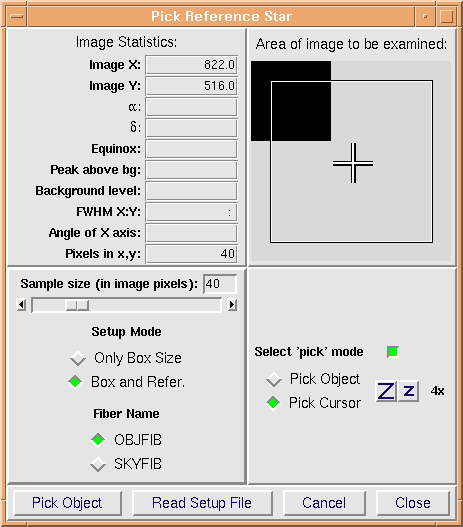
\includegraphics[width=.5\linewidth]{ag/PickRef.png}
\caption[Window to set FEROS fibre reference position]{Window to set \gls{feros} fibre reference position \texttt{Pick reference star}. Select checkbox \texttt{Pick Cursor}.}
\label{fig:pickref}
\end{figure}

\newpage

\subsection{Guiding}
\label{sec:ferosguiding}

\paragraph{On fibre}

The fastest way to guide with FEROS is using the reflection on the fibre head.  It is not adequate for faint stars (try to get $\approx 4\text{--}5000$ counts) or
with bad weather.

\procedure{Guide a FEROS observation using reflection on the fibre head}
\begin{enumerate}
  \item Check that \gls{wfi} \gls{ag} is off.
  \item Centre the target onto the fibre.\\
  In window \texttt{E2P2 Real Time Display}, click \texttt{Centering} below \texttt{Image Control} and click on the target. 
  \item In \texttt{Autoguiding} window, choose integration times (6, 3, $x$ for bright targets with $x < 3$).
  \item Click \texttt{Start guiding}.
\end{enumerate}

It is possible to guide blind using another star of the field in the fibre head viewer.  It is not recommended and should be used as a last resort.

\paragraph{Off fibre}

\procedure{Guide a FEROS observation blindly using off-fibre reference}
\begin{enumerate}
  \item Check that \gls{wfi} \gls{ag} is off.
  \item Centre the target onto the fibre.
  \item Choose integration times (6, 3, $x$ for bright targets with $x < 3$).
  \item Set reference to a star of the field.
  \item Start guiding.
  \item \textbf{Important:}  at the end of the OB, set the reference back to fibre position.
\end{enumerate}

\paragraph{Using WFI}

This is the preferred method in bad weather or for faint targets.  When the FEROS \gls{adc} is used the WFI guide field is extremely defocused and this guiding method may be unstable.

\procedure{Guide FEROS observation with the WFI guide camera}
\begin{enumerate}
  \item Centre the target on the fiber. \\
  In window \texttt{E2P2 Real Time Display}, click \texttt{Centering} below \texttt{Image Control} and click on the target. 
  \item Change filtre to limit the defocus in the \gls{wfi} \gls{ag}
  \begin{enumerate}
    \item Go to the workstation \texttt{WFI BOB}, workspace \texttt{OS GUI}.
    \item In panel \texttt{e2p2 OS GUI}, select filtre under \texttt{SETUP Instrument}.
    \begin{itemize}
        \item If \gls{feros} \gls{adc} is used, select Cousins $I$.
        \item Other wise, use standard $R$.
    \end{itemize}
    \item In the same panel, click apply.
    \item Wait for filtre change ($\approx 1$ min)
      \begin{itemize}
         \item On the panel, field \texttt{Filtre Name} will first display \texttt{Moving}.
         \item When the right filtre name appears, proceed with guiding.
      \end{itemize}
  \end{enumerate}
  \item Proceed with guiding as for a \gls{wfi} \gls{ob} (Sect.~\ref{sec:guidewfi}).
  \item Recentre the target on the fibre
    \begin{enumerate}
       \item Go to the workstation \texttt{Telescope Control Software}.
       \item On the \texttt{TCS Main Panel} find the virtual racket.
       \item Select \texttt{Offset} and tick checkbox \texttt{Combined Offsets}.
       \item Enter offset values for both axes (0.3) and click \texttt{Store}.
       \item Use the arrows to centre if necessary.  
    \end{enumerate}
  \item \textbf{Important:} stop guiding at the end of the \gls{feros} \gls{ob}.\\
  In the\texttt{ TCS Control Panel}, click \texttt{Stop Monitoring} (under \texttt{AG Monitoring Parameters}) and click \texttt{Off} (in the panel \texttt{Autoguider}).  
  %Ivan: and OFF -> Not active?
  \item \textbf{Note:} when observing with the ADC, don't lose time centering on the first pop-up.  No second
     pop-up will be issued after ADC has entered the beam path, so you should
     \texttt{Pause} the exposure if you take time acquiring guiding and centring
     the target.
\end{enumerate}

\section{GROND}

\subsection{Switching to GROND}

You can start an OB once point \ref{list:switch-mcclose} has been done.  This minimises overheads by parallelising preset, mirror movements, and autoguiding configuration.  If the Moon is between the first target and the current position or you are on a bright star, you should manually preset with the main cover closed to avoid blinding the IR detector.

\procedure{Switch to GROND observations}
\begin{enumerate}
  \item Ensure the \gls{grond} main cover is closed to avoid pointing a bright target with open shutters\\
        Your FEROS targets may be very bright or you might slew over the moon in your first GROND observation.\label{list:switch-mcclose}
  \begin{enumerate}
    \item Go to screen \texttt{GROND BOB}.
    \item In a terminal, type \texttt{grondMC CLOSE}.
    \item Wait for cover to close (10-15 s). on panel \texttt{GROND General state}\\
                Due to a big, it will say \texttt{Moving}, \texttt{Open}, then \texttt{Closed}
  \end{enumerate}
  \item There is no need to switch the pointing model to \gls{grond}\\
        GROND does it automatically, but you can do it to be consistent with FEROS and WFI.
  \item To gain time, ensure the \gls{grond} M3 mirror is on \gls{grond}
  \begin{enumerate}
    \item Go to window \texttt{GROND General State} on screen \texttt{GROND BOB}
    \item If \texttt{M3} says WFI\label{list:grond:checkm3}, send it to GROND.\\
            In a terminal, type \texttt{grondM3 GROND} and wait for it to go from \texttt{MOVING} to \texttt{GROND}
  \end{enumerate}
  \item Set up the autoguider on workspace 
  \begin{enumerate}
    \item Go to the \texttt{GROND} workspace of screen \texttt{Autoguider GROND \& FEROS}
    \item Set up the autoguiding properties. (See Fig.~\ref{fig:agswitch})
    \begin{enumerate}
      \item Go to window \texttt{Autoguider},\\
            If necessary open it with \mmenu{CAM user}{Autoguider}.
      \item Change the guiding unit to \gls{grond}\\
            Select \texttt{GROND} under \texttt{Guiding unit} in the \texttt{CCD Control} area. 
      \item Select autoguiding loop times.\\
            Under \texttt{Autoguider control} fill in the numbers from top to bottom\\
            8, 4, 1 is usually fine, then 1 can be increased or decreased (0.001--3.999) depending on guide star.
      \item Restart exposure so that guider takes new values into account.
      \begin{itemize}
        \item If \texttt{CCD Status} is \texttt{Infinite loop}, click \texttt{Stop exposure}
        \item Wait a few seconds for it to change to \texttt{Inactive} (check the exact word)%% TODO
        \item Click \texttt{Start exposure}.
      \end{itemize}
    \end{enumerate}
    \item Set up the autoguider real time image.
    \begin{enumerate}
      \item Go window \texttt{Telescope R.T.D.}\\
              If necessary open it with \wmenu{CAM User}{Autoguider RTD Grond} 
      \item Activate the guide camera image flow if necessary.\\
              Use \wmenu{TCS}{Attach camera}.
      \item Ensure autoguider refreshes image\\
              On the \texttt{Autoguider control} the checkbox \text{Display Enable} should be red
    \end{enumerate}
    \item Ensure the reference picking window \texttt{Pick Reference Star} is open\\
          If necessary open it from \gls{rtd} with \wmenu{TCS}{Pick Reference Star}
  \end{enumerate}
  \item Start the observation
  \begin{enumerate}
    \item Go the the \texttt{bob+gen state} workspace of screen \texttt{FEROS BOB}
    \item In \texttt{bob}, fetch \gls{ob} and click \texttt{Start}
    \item Wait for preset to near or reach target\\
          Look on the Rose Diagram of the \texttt{TCS Setup Panel} on the \texttt{TCS} screen.
    \item Open the main cover
    \begin{enumerate}
      \item Go to screen \texttt{GROND BOB}.
      \item In a terminal, type \texttt{grondMC OPEN}.
      \item Wait for cover to close (10-15 s) by checking value on panel \texttt{GROND General State}\\
            Due to a bug, it will say \texttt{Moving}, \texttt{Closed}, then open \texttt{Open}. 
    \end{enumerate}
    \item Acquire guide star is needed or asked
  \end{enumerate}
\end{enumerate}


\subsection{React to an automatic trigger}

\procedure{React to an automatic trigger}
\begin{enumerate}
  \item Check that your exposure is beeing read out automatically, if not, do it manually
    \begin{itemize}
        \item \textit{(\gls{feros})} click \texttt{END} on \texttt{FEROS Control}
        \item \textit{(\gls{wfi})} click \texttt{END} on \texttt{WFI General State} panel.\\
        If WFI wasn't read out and preset is started, frame is lost.
    \end{itemize}
  \item Click \texttt{OK} on the trigger to start preset.\\
        Preset will be automatic after 30 seconds.
  \item Set up the autoguider (unless you were observing with GROND).\\
        Go to the screen \texttt{Autoguider GROND \& FEROS}
  \item Switch off the \gls{wfi} autoguider if needed
  \begin{enumerate}
    \item Set up the autoguiding properties. (See Fig.~\ref{fig:agswitch})
    \begin{enumerate}
      \item Go to window \texttt{Autoguider}, open it if necessary.\\
            To open: left-click the workspace, choose \texttt{Autoguider} from menu \texttt{CAM user}.
      \item Change the guiding unit to \gls{grond}\\
            Select \texttt{GROND} under \texttt{Guiding unit} in the \texttt{CCD Control} area. 
      \item Select autoguiding loop times.\\
        Under \texttt{Autoguider control} fill in the numbers from top to bottom\\8, 4, 1 is usually fine, then 1 can be increased if necessary.
      \item You may need to \texttt{Start exposure}.
    \end{enumerate}
    \item Set up the autoguider real time image.
      \begin{enumerate}
      \item Go window \texttt{Telescope R.T.D.}, open it if necessary.\\
            To open: left-click the workspace, choose \texttt{Autoguider RTD Grond} from menu \texttt{CAM user}.
      \item Activate the guide camera image flow if necessary.\\
        Use menu \texttt{TCS} $\rightarrow$ \texttt{Attach camera}.
      \end{enumerate}
    \item Ensure the reference picking window is open
      \begin{enumerate}
        \item Look for window: \texttt{Pick Reference Star}\\
              To open: from \gls{rtd} window use menu \texttt{TCS} $\rightarrow$ \texttt{Pick Reference Star}
      \end{enumerate}
  \end{enumerate}
  \item Start the guiding (Sect.~\ref{sec:grond:guide} below).
\end{enumerate}

\subsection{Guiding}
\label{sec:grond:guide}
\procedure{Guide with GROND}
\begin{enumerate}
  \item Chose typical 8, 4, $x$ values in the autoguider, with $x \le 4$.
  \item When \texttt{RTD} has loaded an image, click \texttt{Auto Set Cut Levels}.
  \item In the \texttt{TCS} option, select \texttt{Pick Reference Star}.
  \item Click on a good star at least 100 pixels from the border.
  \item In \texttt{Autoguiding} window, click \texttt{Start guiding}.
\end{enumerate}

\section{All intruments}

\subsection{Run an observing block}

There are three ways to run an OB: use a template in \gls{bob} and modify it on the fly; call it from \gls{p2pp}; call it from the \gls{ot} execution sequence.  The last method allows to automatically fetch and run OBs in a sequence, without lost time, but popups must be attended, of course.



\subsection{Skip the preset}

If the telescope is already on the right target, you can skip the preset when
starting an OB. For observations requiring guiding, you should make sure that
it is already on or acquire it right after the first exposure begins.  On \gls{wfi}, it should be avoided if the observing template sets \texttt{RETURN} to F (false) and pointing position is important.

\procedure{Skip the preset}
\begin{itemize}
    \item Generic method
    \begin{enumerate}
        \item In \gls{bob}, open the aquisition template\\
          Use left click on the triangle.
        \item Edit the PREST field to F\\
          You need to set bob to ``engineering'' mode.\\
          Middle click on the value, it should be T by default.
        \item Start the OB.
        \item Start the guiding if needed\\
              For \gls{wfi}, see quick guiding Procedure~\ref{proc:quickguide}
    \end{enumerate}
    \item Standard observation with FEROS or GROND
    \begin{enumerate}
        \item In \gls{bob}, deactivate the preset template\\
              Use right click on the triangle.
        \item Ensure guiding is working if needed
        \item Start the OB.
    \end{enumerate}
\end{itemize}
    
 
%Ivan: open Protective Shutter to observe?
  
%%%%%%%%%%%%%%%%%%%%%%%%%%%%%%%%%%%%%%%%%%%%%%%%%%%%%%%%%%%%%%%%%%%%%%%%%%

\chapter{Morning: Closing \& Calibrations}
\label{closing}

\section{Panels referred to}
When closing, you may need panels that are not automatically opened at startup. Here is how to find and open them.
\begin{enumerate}
\item On the \gls{tcs} screen, ensure that the \gls{auxfunc} (Fig.~\ref{fig:tcsauxfunc}) is open.\\
      If not, left-click on an empty region and select \texttt{TCS panels} $\rightarrow$ \texttt{Aux Functions}.
\item On the \gls{windows}, ensure mozilla shows the \gls{webcam} (Fig.~\ref{fig:webcam}).\\
      The tab named \texttt{TRENDNET…} can be opened with bookmark \texttt{Dome Webcam}.
\item On the \gls{windows}, ensure mozilla has a tab with \gls{domefunc}.\\
      Tab tab named \texttt{ADAM 6000…} can be opened with bookmark \texttt{Dome Controls} (Fig~\ref{fig:domefunc}).
\end{enumerate}

\section{Telescope}

To put the telescope to a safe parking position one has to follow steps in a definite order, in particular, it is best to close the main mirror cover before anything else. (Except in an emergency closing of the dome.) 

\procedure{Close the dome.}
\begin{enumerate}
\item Close the main mirror cover.\\ 
      In the \texttt{TCS Setup Panel} (Fig.~\ref{fig:tcssetup}), click \texttt{Close} below \texttt{Main Mirror Cover}. 
\item Wait $\approx 2\,$min until it says closed.\\
      In the same panel, it should state \texttt{Closed} below \texttt{Main Mirror Cover}.
\item Park the telescope.\\ 
      In the same panel, click \texttt{Zenith} under \texttt{Fixed preset}.
\item Wait for preset to complete.\\
      In the \texttt{TCS Control Panel}, the telescope should be at the zenith in the rose diagram.
\item Put the dome in manual.\\  
      In the \texttt{TCS Setup panel}, click the \texttt{Manual} checkbox under \texttt{Dome}.
\item Close the slit.\\ 
      In the same panel, click \texttt{Close} under \texttt{Slit}.
\item Switch on the light in the dome (Fig~\ref{fig:webcam}).\\ 
      In the \gls{auxfunc} (Fig.~\ref{fig:tcsauxfunc}), select \texttt{200V} under \texttt{Flat Field Lamp}.
\item Check the slit is closed and telescope at zenith \\
      Use the \gls{webcam} (Fig.~\ref{fig:webcam}) on the mozilla tab \texttt{TRENDNET} on the \gls{windows}.
\item Switch off the light in the dome. \\
      In the \gls{auxfunc}, select \texttt{OFF} under \texttt{Flat Field Lamp}
\end{enumerate}

If the panel is frozen, you can execute commands from a terminal, in directory \texttt{bin}: \texttt{closemirror}, \texttt{presetzenith}, \texttt{closeslit}, \texttt{domemanual}.  Or you can try to revive the panel (See procedure~\ref{proc:unstuckTCSpanel}).

If nothing works, you must ask for support from an ESO TIO.  ESO is still responsible for the safety of the facilities.

\section{Instruments}
One should close the protective shutters of \gls{wfi} and \gls{grond},  cut the communication between instruments 
and \gls{tcs}, and ensure mirrors let light directly to \gls{wfi} for dome flats.

\procedure{Put the instruments offline}
\begin{enumerate}
\item Close the \gls{wfi} protective shutter.\\
      Check on the General State panel in the WFI monitor (Fig.~\ref{fig:wfigen}) that \texttt{Protective Shutter State} is \texttt{CLOSED}.\\
      If not, go to \gls{auxfunc} (Fig.~\ref{fig:tcsauxfunc}) and \texttt{CLOSE} the \texttt{WFI Protective Shutter}.
\item Deactivate \gls{feros} communication.\\ 
      In the FEROS control panel (Fig.~\ref{fig:feroscon}) select from menu \texttt{Telescope} $\rightarrow$ \texttt{IGNORE}.
\item Deactivate \gls{grond} communication.\\ 
      In the GROND Control panel (Fig.~\ref{fig:grondcon}), click \texttt{RRM STANDBY} and \texttt{TCS OFF}
\item With \gls{grond}, close the cold and protective shutters.\\ 
      In a terminal, type \texttt{grondCS CLOSE} and \texttt{grondMC CLOSE}.
\item Ensure \gls{feros} mirror is not in the way.\\
      In panel FEROS Control (Fig.~\ref{fig:feroscon}), \texttt{M3 Selection Mirror} should state \texttt{WFI}\\
      If not, int the \gls{ics} control panel (Fig.~\ref{fig:ferosics}), check the \texttt{mirr3} box, select \texttt{WFI}, click \texttt{SETUP}.
\item Ensure \gls{grond} mirror is not in the way.\\
      In panel  GROND Control (Fig.~\ref{fig:grondcon}), \texttt{GROND M3} should state \texttt{WFI}.\\
      If not, type \texttt{grondM3 WFI} in a terminal.
\end{enumerate}


\section{Dome}

Turn off ventilation and hydraulics using the \gls{domefunc} (\gls{windows}, Fig.~\ref{fig:domefunc}). If it is required, use the good seeing password.
\begin{enumerate}
  \item Turn off the dome ventilation.\\
        Click \texttt{Dome Air} if the button just above it is green.
  \item Turn off the hydraulics.\\
        Click \texttt{HydrOff}. The button above \texttt{Hydr} should go red. 
\end{enumerate}

\section{Tidying folders}

Scripts move the data of the previous nights are to a subdirectory directory and and remove old ones (already in the ESO archive) if disk space is needed.  It can be done any time (night, day) on a daily basis for WFI and FEROS.  The GROND team manages the data.

\procedure{Tidy folders}
\begin{enumerate}
  \item On the \gls{wfi} screen, type \~{}\texttt{/bin/sciopsTidyMess.sh} in a terminal (wfi xterm).
  \item On the \gls{feros} screen, type \~{}\texttt{/bin/sciopsTidyMess.sh} in a terminal.
\end{enumerate}

\section{Health checks \& internal calibrations}
\label{sec:clocal}

Lauch health checks and internal calibrations.

\procedure{Launch morning health checks and internal calibrations}
\begin{enumerate}
  \item Run \gls{feros} linearity check.\\
        In \gls{bob}, load and run the daily linearity OB using \texttt{Fetch an OB from file}.\\
        Name is \texttt{linearity-\#-weekday} where \texttt{weekday} is that at the start of the night.
  \item Run the \gls{wfi} health check, biases, and dark.\\
        In \gls{bob}, load and run the daily calibration OB using \texttt{Fetch an OB from file}.\\
        Name is \texttt{WFI\_cal\_\#-weekday} where \texttt{weekday} is that at the start of the night.
  \item Run \gls{grond} calibrations.\\
        In \gls{grond} \gls{bob}, load and run \texttt{GROND\_cal.obd} using \texttt{Fetch an OB from file}\\ 
        (\texttt{.../TEMPLATES/OBD/}). 
\end{enumerate}




%----------------------------------------------------------------------------------------

\chapter{Managing observing blocks}
\label{ob}

\section{Transferring OBs from one's laptop}

\subsection{Standard way}

\procedure{Transfer OBs from one's computer to the telescope, using p2pp check-in}
\begin{itemize}
\item On your laptop's \gls{p2pp} select all your \glspl{ob}.
\item Use menu \texttt{File} $\rightarrow$ \texttt{Check-in}
\item Use menu \texttt{Readme} $\rightarrow$ \texttt{CheckIn Readme} if necessary
\item If using \gls{ot} (advised)
  \begin{itemize}
    \item From main \gls{ot} window, use menu \texttt{Queues} $\rightarrow$ \texttt{Repository Browser}
    \item Select \texttt{OB name} checkbox in the Repository Browser window
    \item Empty all fields and enter your \gls{p2pp} username  
    \item Click \texttt{Query}
    \item Select all the \glspl{ob} you need with the mouse (they should have status Defined)
    \item Select \texttt{Mark Status} and chose \texttt{(V)erified}
    \item Select the same \glspl{ob} again
    \item Append to queue, typically \texttt{MPIA-YYYY-MM} (named by year and month)
    \item Find the window corresponding to this queue and use \texttt{Menu} $\rightarrow$ \texttt{Save}
  \end{itemize}
\item If using \gls{p2pp}
  \begin{itemize}
    \item TBW
  \end{itemize}
\end{itemize}

\subsection{Loading manually}
If this fails, for instance for \glspl{ob} longer than one hour, you should
ssh them from your laptop and load them manually into the dhs computer.

\procedure{Transfer OBs from one's computer to the telescope, using manual file transfer.}
\begin{itemize}
  \item Check that your laptop accept ssh connections.
  \item Connect it to the cable network.
  \item Find your laptop's IP address.  With linux or mac, 
        \texttt{/sbin/ifconfig} or \texttt{ifconfig} should give it.
  \item On the \gls{p2pp} machine create a directory let's say \texttt{~/yourname/OBs} 
  \item On the same machine, type \texttt{scp -r yourlogin@youripaddress:pathtoOBs ~/yourname/OBs}
        and type your password.
  \item Open \gls{p2pp} with your credentials
  \item Select your program ID on the left column
  \item Use menu \texttt{File} $\rightarrow$ \texttt{Import}
\end{itemize}

Note: if you cannot activate ssh services on your laptop, use a USB stick and someone else's computer.   Alternatively, send an e-mail you will open on the p2pp machine (not advised). 

\section{OT}
%Ivan: completar

On the \gls{p2pp} machine, there is a workspace to use OBs from the observing tool (\gls{ot}). In the \texttt{Repository Browser} of the \gls{ot}, find your OB using fields such as instrument, period, ID, username, position, etc.  Click on the OB and then on a tab called \texttt{Execution Sequence} that it is in the same panel.

There should be an open window which is called \texttt{Execution Sequence}. The selected OB will be listed there, maybe with a list of others. Use the buttons \texttt{move up} (or \texttt{move down})  to move the OB you want to run next to the top of the list since it has to be the first one.

Then, go to \gls{bob} and use the menu \texttt{Configure} $\rightarrow$ \texttt{Environment}. In the \texttt{Process} tab change \gls{p2pp} by \gls{ot}. Now you can fetch the OB from \gls{ot}.


%\section{BOB}

%----------------------------------------------------------------------------------------

\chapter{Software maintenance}
\label{sec:reboots}

\section{Monthly}

About once a month a weekly software maintenance should be done for prophyllaxy.

\procedure{Monthly software maintenance}
\label{proc:monthly}
\begin{enumerate}
\item \label{list:soft:stop} Stop some processes and applications (2 min)
  \begin{enumerate}
     \item On the p2pp/ot screen, exit applications
     \begin{enumerate}
      \item Locate the main \gls{ot} window with the execution sequence and exit it.
      \item Locate any open \gls{p2pp} window and exit it
     \end{enumerate}
     \item On the pipeline screen, stop pipeline processes
             \begin{enumerate}
                \item Open or locate a terminal
                \item Type \texttt{doControl stop}
                \item Type \texttt{stopRBS}
             \end{enumerate}
     \item On the FEROS DRS screen, stop data processes following the first two points of Procedure~\ref{sec:FEROSDRSrestart}
             \begin{enumerate}
                \item Stop and close the Data subscriber and the FEROS DRS panel (point~\ref{list:stopDRS})
                \item Kill processes and remove lock files (point~\ref{list:killDRS})
             \end{enumerate}
   \end{enumerate}
\item \label{list:soft:exit} Exit all sessions except \gls{grond} (1 min)
    \begin{enumerate}
        \item On the \gls{tcs} screen, exit the X environment
        \item On the \gls{wfi} screen, exit the X environment
        \item On the \gls{feros} screen, exit the X environment
        \item On the GROND and FEROS \gls{ag} screen, exit the X environment
        \item On the \gls{grond} screen, exit the X environment
        \item On the p2pp/ot screen, exit the X environment
        \item On the pipeline workstation, exit the X environment
        \item On the FEROS DRS workstation, exit the X environment
    \end{enumerate}
\item \label{list:soft:power}Power cycle all black Dell boxes except \gls{grond}'s (2 min) 
\item Log into all sessions (2 min)
\begin{enumerate}
    \item On the \gls{tcs} screen, login as \texttt{tcs}
    \item On the \gls{wfi} screen, login as \texttt{wfi}
    \item On the \gls{feros} screen, login as \texttt{feros}
    \item On the FEROS and GROND AG screen, login as \texttt{cam}
    \item On the GROND screen, login as \texttt{grond}
    \item On the \gls{p2pp}/\gls{ot} workstation, login as \texttt{dhs}
    \item On the pipeline workstation, login as \texttt{pipeline}
    \item On the FEROS \gls{drs} workstation, login as \texttt{astro}
\end{enumerate}
\item Reboot workstations (except GROND)
\begin{enumerate}
    \item On the \gls{tcs} screen, open a tcs terminal and type \texttt{reboot}
    \item On the \gls{wfi} screen, open a wfi terminal and type \texttt{reboot} 
    \item On the \gls{feros} screen, open a feros terminal and type \texttt{reboot}
    \item On the FEROS DRS screen, open a terminal type \texttt{reboot} as root
    \item On the pipeline screen, open a terminal type \texttt{reboot} as root
    \item On the p2pp/ot screen, open a terminal type \texttt{reboot} as root
\end{enumerate}
\item Wait for the reboots to complete (20--30 min). You can check with any of the following:
    \begin{itemize}
        \item The terminal disappears when clicked on
        \item From a grond terminal, type \texttt{ping <machine>}.
             \begin{itemize}
             \item <machine> can be w2p2tcs, w2p2ins (WFI), wferos, w2p2dhs (OT/p2pp), w2p2pl (pipeline), w2p2off (FEROS DRS). 
             \item Reboot is not done if \texttt{No route to host} is answered.
             \item When ping starts sending internet speed stats reboot is almost complete (less than one minute left).
             \end{itemize}
    \end{itemize}
\item Restart some processes and applications
    \begin{enumerate}
        \item On the \gls{p2pp}/\gls{ot} screen, open \gls{ot}
        \item On the pipeline workstation
             \begin{enumerate}
                \item Open  a terminal
                \item Type \texttt{dhsSubscribeControl start pipeline -backsince <date>}\\
            pick <date> a few days ago
                \item Type \texttt{doControl start wfi,feros}
                \item Type \texttt{startRBS pipeline.config}
             \end{enumerate}
        \item On the FEROS DRS workstation, follow the last point of Procedure~\ref{sec:FEROSDRSrestart} in order to
             \begin{enumerate}
                \item Open and configure data subscriber (point~\ref{list:DS})
                \item Open the FEROS DRS panel (point~\ref{list:DRS})
             \end{enumerate}
    \end{enumerate}
\item \label{list:soft:tcs}Perform a full \gls{tcs} restart
\end{enumerate}

\section{Every six months}

Every six months a weekly software maintenance has an additional step with the reboot of the user workstation.

\procedure{Monthly software maintenance}
\begin{enumerate}
\item Stop processes and exit sessions (steps~\ref{list:soft:stop}--\ref{list:soft:exit} of Procedure~\ref{proc:monthly})
\item Have a reboot of the user workstation done (15 min?)
    \begin{enumerate}
        \item Contact IT at Paranal (Josefina Urrutia) 
        \item Coordinate a reboot of user workstation \texttt{uws2p2}
        \item Wait for their confirmation that it is done
    \end{enumerate}
\item Power cycle dell boxes, log into sessions, reboot workstations, restart processes, and start-up TCS (steps~\ref{list:soft:power}--\ref{list:soft:tcs})
\end{enumerate}


\chapter{Troubleshooting}
\label{sec:trouble}

\section{No flux or little flux}
\label{sec:noflux}

\procedure{Investigate and fix the reason for the absence of flux in an instrument}. Ensure that
\begin{itemize}
  \item the slit is \texttt{OPEN} (\gls{tcs} setup, Fig.~\ref{fig:tcssetup}).
  \item the dome is on automatic (\gls{tcs} setup,
        Fig.~\ref{fig:tcssetup}) and the slit is aligned (\gls{tcs}, Fig.~\ref{fig:tcs}).
  \item the Main Mirror Cover is \texttt{OPEN} (\gls{tcs} setup,
        Fig.~\ref{fig:tcssetup}).
  \item the \texttt{mirr3} mirror is on \texttt{WFI} or \texttt{FEROS} (\gls{feros} \gls{ics}, 
        Fig.~\ref{fig:ferosics}) if observing with \gls{wfi} or \gls{feros}.  If necessary,
        click its checkbox and \texttt{SETUP}.
  \item the M3 mirror is on \gls{grond} if observing with \gls{grond} and on \gls{wfi} otherwise
         (\gls{grond} control, \ref{fig:grondcon}).  Use 
        \texttt{grondM3 WFI} or \texttt{grondM3 GROND} in the terminal if
        necessary.
  \item \textit{(\gls{wfi})} the protective shutter is \texttt{OPEN} (\gls{auxfunc} 
        on the \gls{tcs} machine, \ref{fig:tcsauxfunc}). 
  \item \textit{(\gls{grond})} the protective and cold shutters are \texttt{OPEN} (\gls{grond} control,
        Fig.~\ref{fig:grondcon}).  Use \texttt{grondMC OPEN} and \texttt{grondCS OPEN} in the terminal if necessary.
  \item \textit{(\gls{grond})} If images look like biases, restart \gls{fiera}.\\
  On the \texttt{FIERA Control Panel} do \texttt{Shutdown} / \texttt{Startup}.
\end{itemize}

\section{Autoguider camera fails}
\label{sec:agfail}

\begin{figure}[p!]
\subfigure[\text{Rack tower}]{
    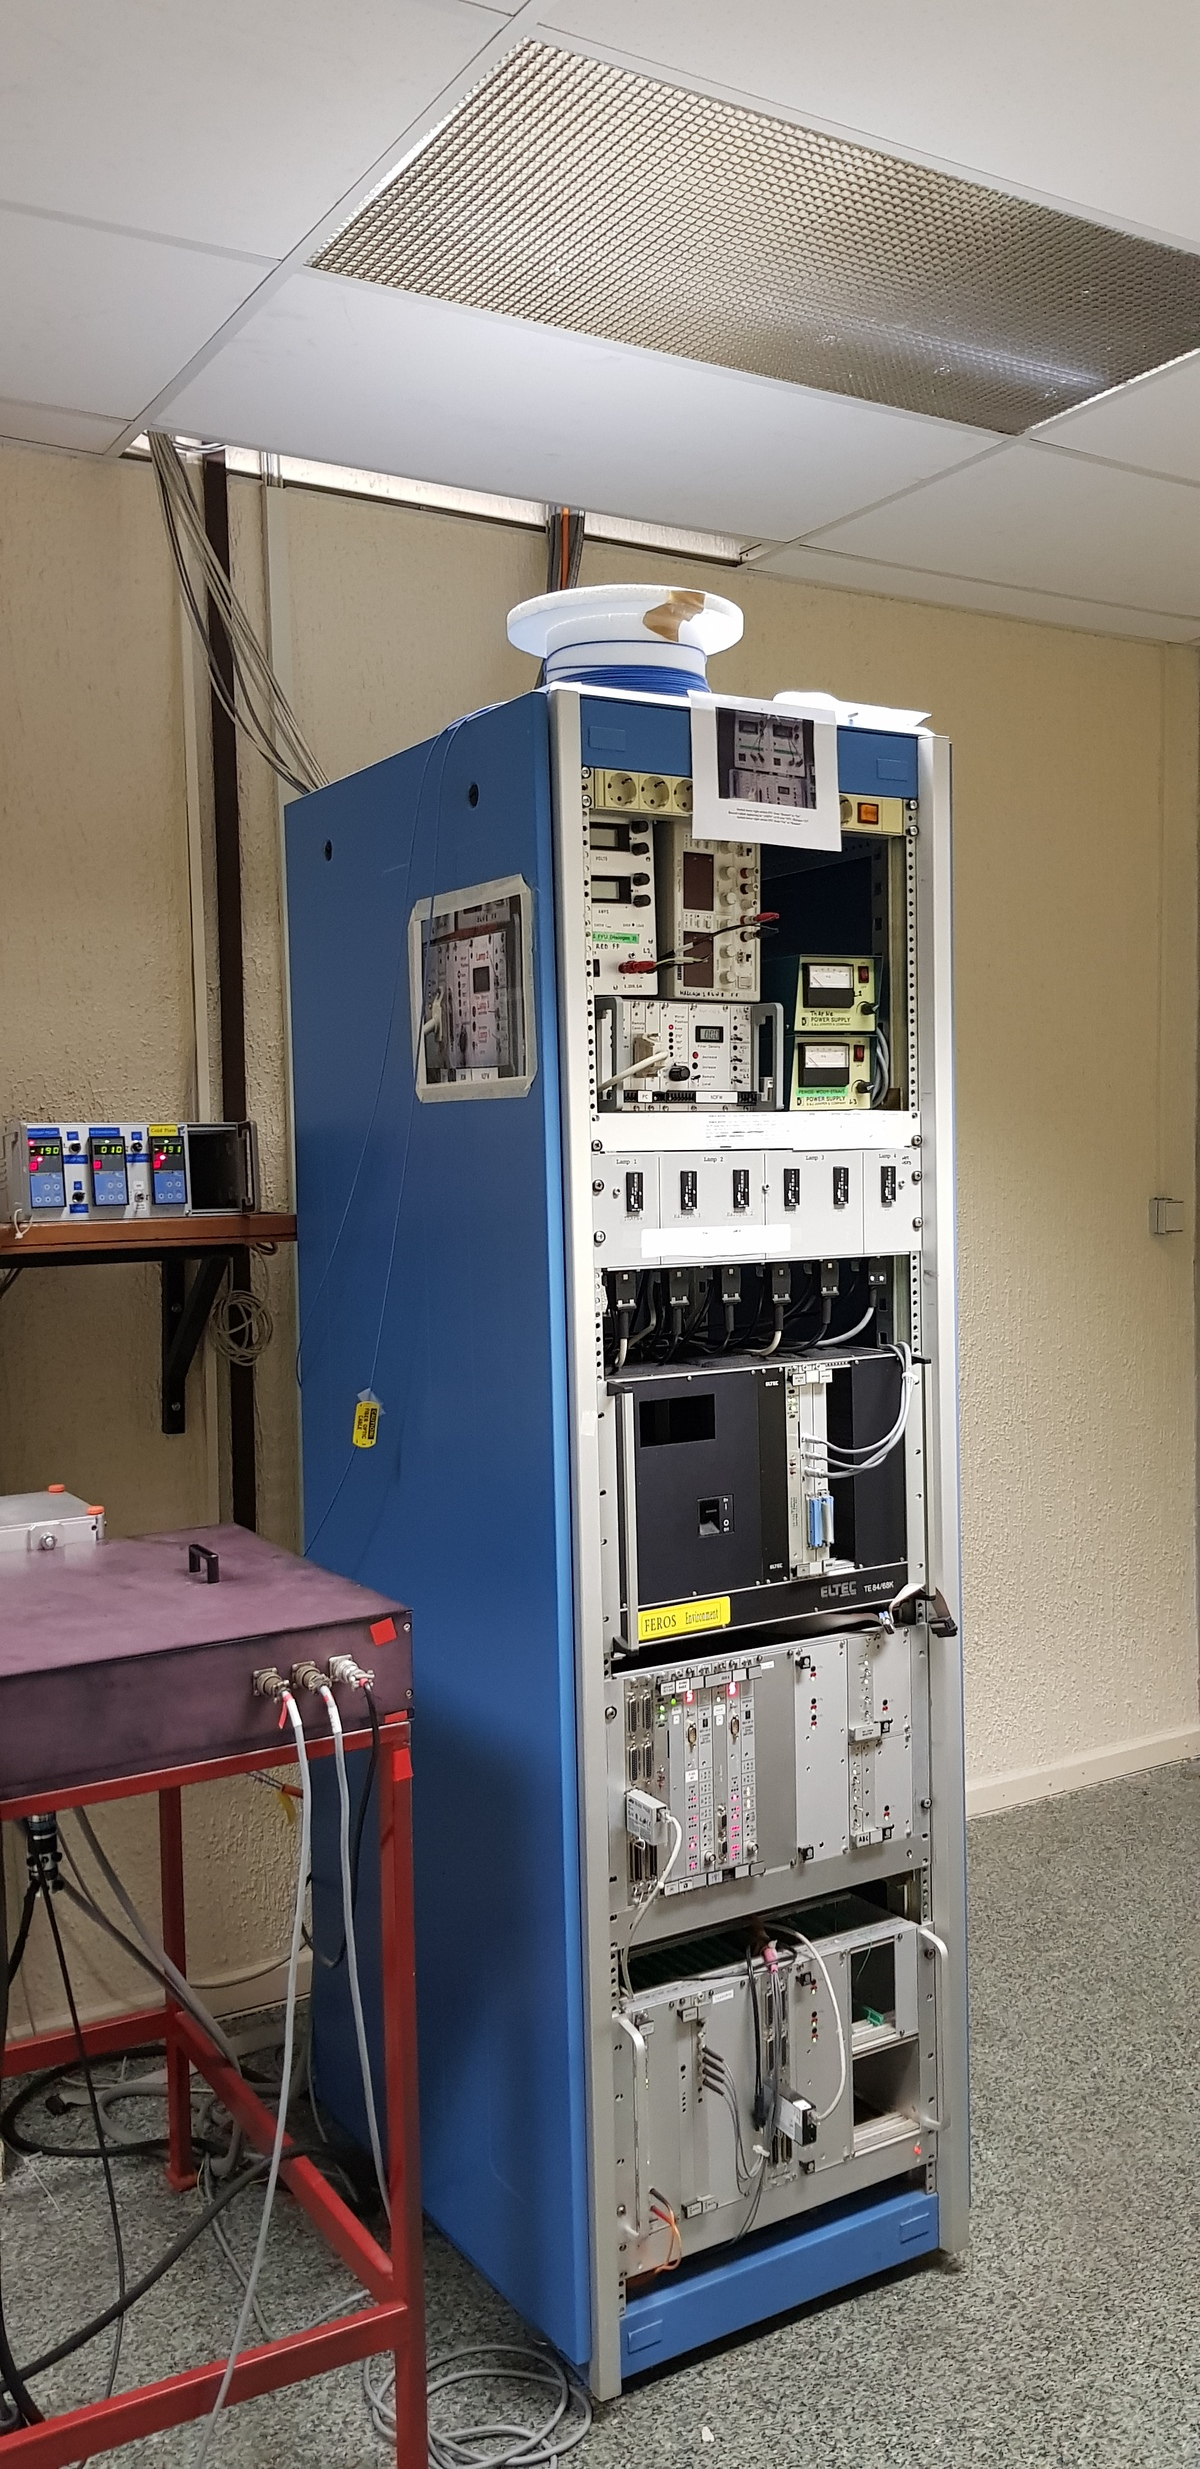
\includegraphics[width=0.3\linewidth]{feros/l2p2cam-rack.jpg}%
    \label{fig:l2p2cam-rack}%
}\hfill
\subfigure[\text{l2p2cam reset}]{
    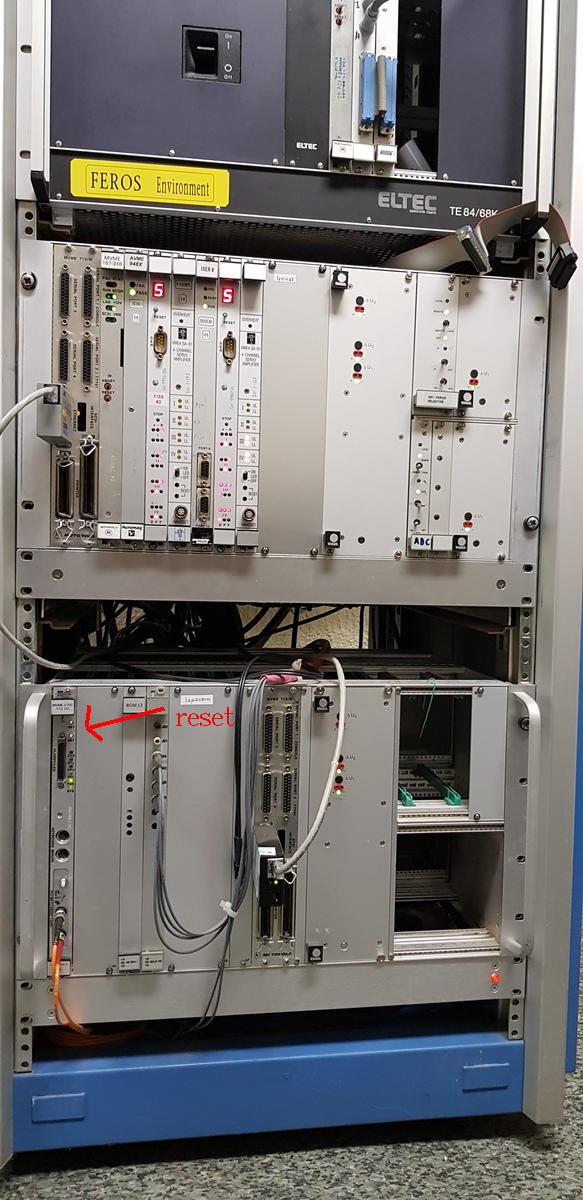
\includegraphics[width=0.3\linewidth]{feros/l2p2cam-front.jpg}%
    \label{fig:l2p2cam-rst}%
}\hfill
\subfigure[\text{l2p2cam power cycle}]{%
    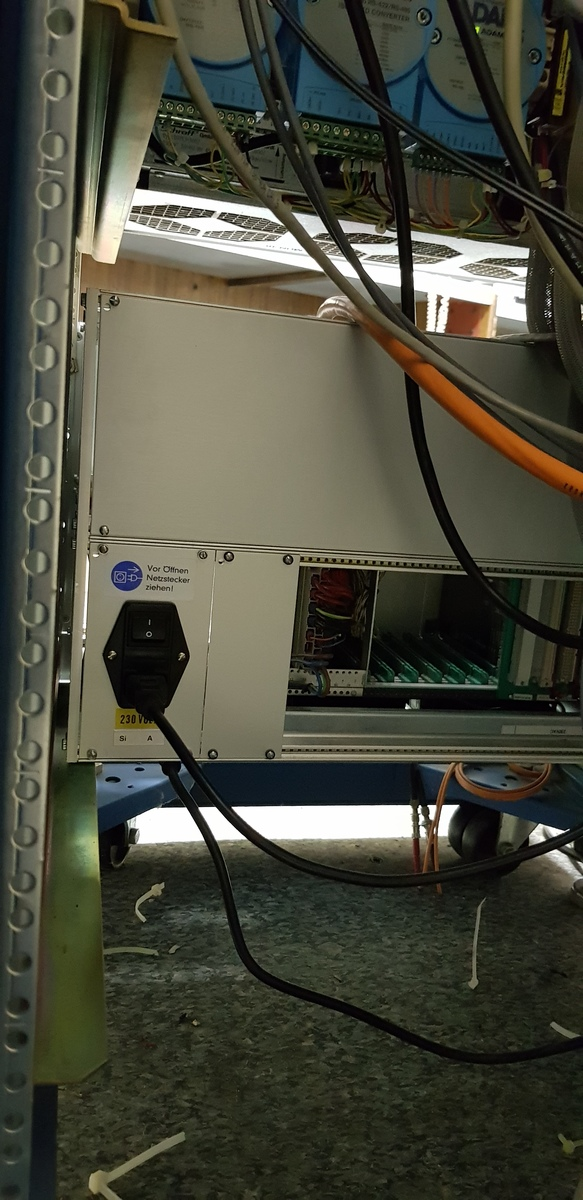
\includegraphics[width=0.3\linewidth]{feros/l2p2cam-back.jpg}%
    \label{fig:l2p2cam-pow}%
}
\caption[Rack with FEROS AG LCU]{Rack with the \gls{feros} \gls{ag} \gls{lcu}.}
\label{fig:l2p2cam}
\end{figure}

\begin{figure}[p!]
\begin{minipage}{0.48\linewidth}
\subfigure[\texttt{scanei}]{%
  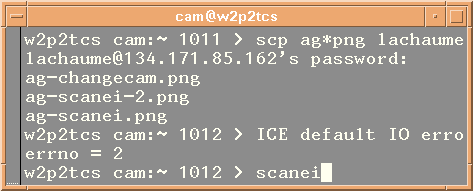
\includegraphics[width=\linewidth]{ag/ag-scanei-0.png}
}\\
\subfigure[Click on l2p2cam or l2p2agr (top right)]{%
  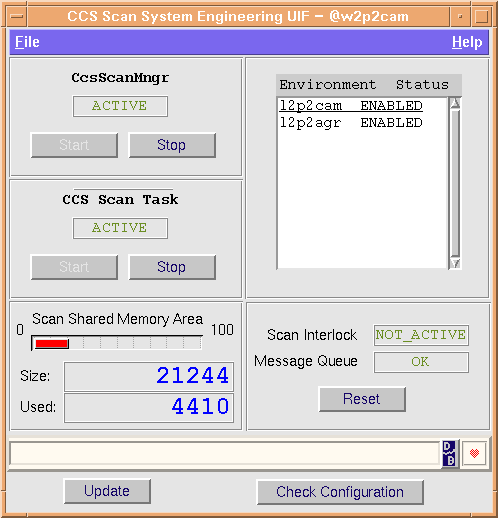
\includegraphics[width=\linewidth]{ag/ag-scanei-1.png}
}
\end{minipage}
\hspace{0.02\linewidth}
\begin{minipage}{0.48\linewidth}
\subfigure[Click enable or disable (top left)]{%
  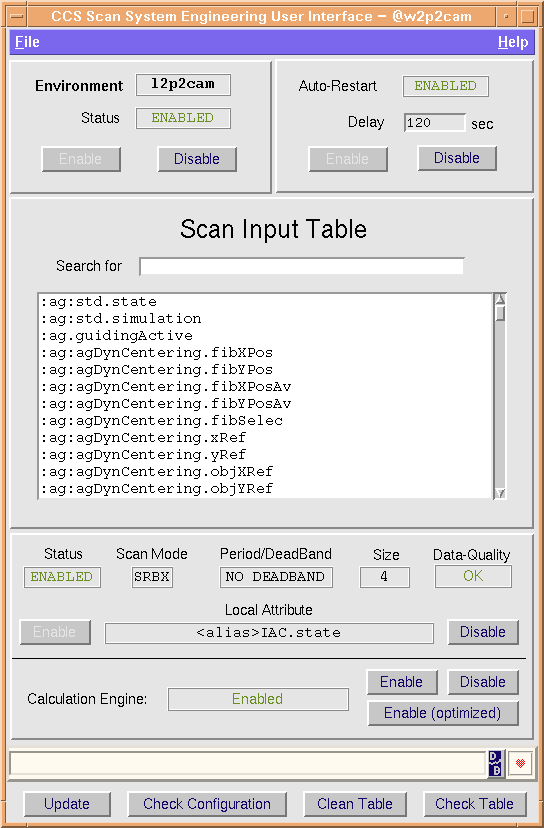
\includegraphics[width=\linewidth]{ag/ag-scanei-2.png}
}
\end{minipage}
\caption[Command scanei to control environments]{\texttt{scanei} on the \gls{feros} and \gls{grond} 
\gls{ag} machine.}
\label{fig:agscanei}
\end{figure}


The \gls{grond} and \gls{feros} autoguider use the same system on screen \texttt{Autoguider GROND \& FEROS}, between the GROND and FEROS screens.  \gls{wfi} has its own system on screen \texttt{Telescope Control Software}.

It is possible to go on observing with GROND and FEROS while restarting the autoguider, provided that the modules are deactivated on the \gls{tcs}. However, you need to reactivate them to do the last step of restarting the autoguider (\texttt{e2p2StartTCCDs}).

\procedure{Observe when the autoguider fails}
\label{proc:agmodules}
\begin{enumerate}
    \item On screen \texttt{Telescope Control Software} go to texttt{Status} workspace
    \item On the \texttt{TCS Status} panel locate the modules section (Fig.~\ref{fig:tcsstatus})
    \item Check ignore for the corresponding modules
    \begin{itemize}
        \item For \gls{grond}, \texttt{ag\_ccdGRND} and \texttt{ccdGRND}
        \item For \gls{feros}, \texttt{ag\_ccdGRND} and \texttt{ccdGRND}
    \end{itemize}
    \item Remember to uncheck them for \texttt{e2p2StartTCCDs} to work!
\end{enumerate}

\subsection{GROND}
If you want to observe while fixing the issue you need to deactivate the modules in the \gls{tcs}, see Procedure~\ref{proc:agmodules}.  You will need to uncheck them just before starting the guider software with \texttt{e2p2StartTCCDs}.

\procedure{Restart the GROND autoguider}
\begin{enumerate}
   \item\label{list:gag1} If in a hurry try the quick restart (1--2 min)
   \begin{enumerate}
       \item On screen \texttt{Autoguider GROND \& FEROS}, find or open a terminal.
       \item Type \texttt{e2p2StopTCCDs gag} and wait for command to finish
       \item Type \texttt{e2p2StartTCCDs gag} and wait for command to finish
   \end{enumerate}
   \item If you have time or \ref{list:gag1} does not solve the issue,
   go for the full restart (3--4 min)
   \begin{enumerate}
       \item On screen \texttt{Autoguider GROND \& FEROS}, find or open a terminal.
       \item Type \texttt{lccBoot l2p2agr}
       \item Wait for the command to finish (1--2 min)
       \item Type \texttt{scanei} to open the scanei GUI
       \begin{enumerate}
	   \item Check that l2p2agr is \texttt{ENABLED}
	   \item If not, enable l2p2agr (see Fig~\ref{fig:agscanei})
	   \item Close the GUI
       \end{enumerate}
       \item Type \texttt{e2p2StartTCCDs gag}
   \end{enumerate}
\end{enumerate}

\subsection{FEROS}
If you want to observe while fixing the issue you need to deactivate the modules in the \gls{tcs}, see Procedure~\ref{proc:agmodules}.  You will need to uncheck them before starting the guider software with \texttt{e2p2StartTCCDs} (step~\ref{lab:fag2}). 

\procedure{Restart the FEROS autoguider}
\label{proc:restartfag}
\begin{enumerate}
    \item Restart the \gls{ag} software (1--2 min).
        \begin{enumerate}
            \item\label{lab:fag0} On screen \texttt{Autoguider GROND \& FEROS}, find or open a terminal.
            \item Type \texttt{e2p2StopTCCDs fag}
            \item\label{lab:fag1} Type \texttt{e2p2StartTCCDs fag}
            \item\label{lab:fag2} Wait for about 1--2 min for the command to exit succesfully.
        \end{enumerate}
    \item If the problem persists or an error pops up in step~\ref{lab:fag2}, reboot the \gls{ag} \gls{lcu} (3--4 min) 
        \begin{enumerate}
            \item Type \texttt{lccBoot l2p2cam}
            \item Type \texttt{scanei} to open the scanei GUI
            \begin{enumerate}
                \item Check that l2p2cam is ENABLED
                \item If not enable l2p2cam (see Fig~\ref{fig:agscanei})
                \item Close the GUI
            \end{enumerate}
            \item Perform steps \ref{lab:fag0}, \ref{lab:fag1}, \ref{lab:fag2}.
        \end{enumerate}
    \item If the problem persists or an error pops up in step~\ref{lab:fag2}, perform a hardware reset of the \gls{lcu} (15 min)
    \begin{enumerate}
       \item Go to the FEROS room located in the telescope enclosure. 
       \item Locate the big blue rack tower (Fig.~\ref{fig:l2p2cam-rack}).
       \item On the lower racks, near to l2p2cam label, push a small RST button (Fig.~\ref{fig:l2p2cam-rst}).
       \item Perform steps \ref{lab:fag0}, \ref{lab:fag1}, \ref{lab:fag2}.
    \end{enumerate}
    \item If this does not solve the issue, power cycle the \gls{lcu} (15 min)
    \begin{enumerate}
        \item Go to the FEROS room located in the telescope enclosure. 
        \item On the back of the rack tower, unplug and replug the lower rack (Fig.~\ref{fig:l2p2cam-pow}).
        \item Perform steps \ref{lab:fag0}, \ref{lab:fag1}, \ref{lab:fag2}.
    \end{enumerate}
\end{enumerate}

\subsection{WFI}
Failure of the \gls{wfi} autoguider will generally be silent.  It will just do nothing when asked to retrieve field or start monitoring.

If the quick 30 seconds fix does not work, it is not possible to observe with WFI during the 15--35 minute-long fix, but it should be possible to go on with GROND or FEROS with no guarantee though---the \gls{tcs} has the bad habit of communicating with the WFI computers for focus. 

\procedure{Fix WFI autoguider issues}
Try in this order
\begin{enumerate}
  \item\label{wfiagrestart}
       On the \gls{tcs} screen, restart the autoguider (30 s)
    \begin{enumerate}
       \item Use left-click menu \texttt{Stop Autoguider}
       \item Use left-click menu \texttt{Start Auoguider}
    \end{enumerate}
  \item If \texttt{Retrieve Field} gives the error \texttt{Error opening RPC connection}, restart the WFI technical CCD.
    \begin{enumerate}
       \item On the WFI screen, locate or open a terminal.
       \item Type \texttt{wfinsStopTCCDS} and wait for it to complete
       \item Type \texttt{wfinsStartTCCDS} and wait for it to complet (2 min)
       \item Perform the AG restart of point~\ref{wfiagrestart}
    \end{enumerate}
  \item If an autoguider process is suspended, restart the \gls{tcs}
    \begin{enumerate}
       \item In a terminal, type \texttt{i}
       \item If there is an AG-related suspended proces, proceed as follow
       \item Deactivate the connection between \gls{feros} and TCS
           \begin{itemize}
                \item On the \gls{feros} screen (Fig.~\ref{fig:saladecontrol}), locate the \gls{feros} control panel (Fig.~\ref{fig:feroscon})
                \item From menu select \texttt{Telescope $\rightarrow$ IGNORE}
           \end{itemize}
       \item Perform a full restart the \gls{tcs} including VME reboot (Sect.~\ref{proc:startup})
       \item Reactivate the connection between \gls{feros} and TCS
           \begin{itemize}
                \item On the \gls{feros} screen (Fig.~\ref{fig:saladecontrol}), locate the \gls{feros} control panel (Fig.~\ref{fig:feroscon})
                \item From menu select \texttt{Telescope $\rightarrow$ ENABLE}
           \end{itemize}
    \end{enumerate}
  \item Reboot the \gls{wfi} SPARC station and dependencies (15--35 min).
    \begin{itemize}
        \item From a terminal type \texttt{rlogin wwffcd -l fcdrun}
        \item Once logged in, type \texttt{reboot}
        \item Wait for reboot to complete (a few minutes)\\
              In a terminal type \texttt{ping wffcd} and wait until it shows packets.
        \item Reboot \gls{wfi} computer (a few minutes)\\
              On screen \texttt{Wide Field Imager}, type \texttt{reboot} in a terminal.
        \item Do the \gls{wfi} weekly startup (10 min)
        \item Restart the TCS or just autoguider (see point 1 \ref{wfiagrestart}), not sure here if TCS restart is needed.
    \end{itemize}
\end{enumerate}

\section{OB doesn't work}

\subsection{OB gives an error when started}

If an OB issues an error within seconds of being started.

\procedure{Fix OB start error}
\begin{enumerate}
  \item If OB was already executed or aborted, click \texttt{Reset status}. 
  \item Check that the object is observable (above 20 degrees).
  \item If telescope preset is needed, check that the communication with the \gls{tcs} is on
    \begin{itemize}
       \item \textit{(\gls{feros})} Use menu \texttt{Telescope} $\rightarrow$ \texttt{Enable}.
       \item \textit{(\gls{grond})} Click \texttt{TCS ON}.
    \end{itemize}
  \item If telescope preset is not needed (e.g. calibrations), deactivate it in 
    \begin{itemize}
      \item \textit{(\gls{feros}, \gls{grond})} Right-click the triangle of the acquisition template.
                   (A thumb down should appear.  If you get a stop, go on clicking.)
      \item \textit{(\gls{wfi})} Set \texttt{PRESET.NEW} to \texttt{F} in the acquisition template.\\
         (This needs menu \texttt{Interface} $\rightarrow$ \texttt{Engineering}.) 
    \end{itemize}
\end{enumerate}

\subsection{OB stalls before starting to observe}

\procedure{Fix stalling of an OB}
\begin{itemize}
\item \textit{(\gls{wfi},\gls{feros})} Try to find a hidden pop-up asking for interaction (behind a window).
\item \textit{(\gls{wfi})} If OB stalls when focus order is sent by \gls{bob},
set it manually.\\
In the TCS screen, enter focus value in the main panel (Fig.~\ref{fig:tcs}).\\
Note: A permanent fix is to restart the \gls{tcs} (see Sect.~\ref{sec:tcsrestart}).
\item \textit{(\gls{grond})} If IR exposure does not start after the optical one has, reset the IR flip mirror.\\
In a terminal, type \texttt{grondFM}
\end{itemize}

\subsection{Crash before an exposure}
\label{sec:expocrash}

Here are possible fixes, from shortest to longest.  Try each one in this
order, until problem is fixed.

\procedure{Investigate and fix a crash ocurring before the start of an optical exposure}
\begin{enumerate}
  \item Close \gls{bob} and launch a new one.
  \item \gls{feros}
    \begin{enumerate}
      \item Restart \gls{fiera}\\
            On the \texttt{FIERA Control Panel} do \texttt{Shutdown} / \texttt{Startup}.
            \label{restartfiera}
      \item Restart the instrument with telescope enabled\\
            (In particular if the second exposure of the night fails.)
         \begin{enumerate}
            \item On the \texttt{FEROS Control} panel, use menu \texttt{Telescope} $\rightarrow$ \texttt{enabled}.
            \item Do the full start-up procedure.
         \end{enumerate}
    \end{enumerate}
  \item \gls{grond}
    \begin{enumerate}
       \item If error \texttt{closing w2p2cam environment}
       \begin{enumerate}
          \item If a \gls{fiera} exposure is running in \texttt{GROND Control}, click \texttt{End} or let it finish.
          \item Type \texttt{grondSHUTTER} in a terminal.
       \end{enumerate} 
       \item If the error mentions \gls{irace}
       \begin{enumerate}
            \item Go to monitor \texttt{GROND IRACE}.
            \item Locate the \texttt{Infrared Acquisition Module} (Fig.~\ref{fig:grondirace})
            \item Click \texttt{Reset} on the lower left part of the panel
            \item Select from menu \texttt{Online} $\rightarrow$ \texttt{Online}
            \item If it fails, you may need $\approx 40$\,min to deep restart (Procedure~\ref{proc:iracerestart}) \gls{irace}.
       \end{enumerate}
       \item Ensure only one \gls{bob} is running
         \begin{enumerate}
           \item Find all \glspl{bob} (\texttt{ps gaux | grep bob})
           \item \texttt{kill} them
           \item launch a new \gls{bob}.
         \end{enumerate}
       \item \textit{(\gls{grond})} Restart \gls{fiera} (see ~\ref{restartfiera}).
       \item \textit{(\gls{grond})} Restart \gls{grond}.
         \begin{enumerate}
           \item Type \texttt{grinsStop}
           \item Type \texttt{grinsStart}
           \item In \texttt{GROND Control} panel, put instrument \texttt{ONLINE}.
         \end{enumerate}
       \item \textit{(\gls{grond})} Reboot \gls{grond}.
       \item \textit{(\gls{grond})} If the GROND control has many TCS-related fields with gray background or the error says something about the FITS keyword TELESCOP, a last resort reboot of GROND may be needed. \textbf{BUT} in case of the first scenario, take a separate exposure with \gls{fiera} (in the control panel) first and check if these fields turn back to their usual color.
     \end{enumerate}
  \item\label{list:wfiexpocrash} \gls{wfi}
    \begin{enumerate}
      \item Abort a possible running exposure manually, in particular if \gls{bob} issues the error message
             ``Cannot start exposure before the last one has read out'' or some
             equivalent message (10~sec)
        \begin{enumerate}
           \item On the \texttt{e2p2 OS GUI} (Fig.~\ref{fig:wfios}) click \texttt{Abort Exp./Seq.}
           \item The GUI should display the text \texttt{ABORT    > INVOKED}
           \item Wait for a few seconds for the answer \texttt{ABORT    > REPLY/ L   OK}.
           \item If it works, problem is solved, if not go to next point.
        \end{enumerate}
      \item Do a \texttt{DAILY} startup of \gls{wfi} (5~min).
      \item\label{list:wfifierarestart} Do a full restart of \gls{fiera} and \gls{wfi} (10-15~min).
        \begin{enumerate}
          \item Go to a \texttt{wfi} terminal or open it from menu \texttt{wfi xterm}.
          \item Shut down the instrument.\\
                Type \texttt{wfinsShutDown}
          \item Check that the environment are enabled.
             \begin{enumerate}
               \item Type \texttt{scanei \&} 
               \item Go to the opening GUI titled \texttt{CSS Scan System}.
               \item Check that \texttt{wwffcd} and \texttt{w2p2tcs} are \texttt{ENABLED}
               \item If either environment is \texttt{DISABLED}, proceed with these points
               \item Click on \texttt{DISABLED}
               \item In emerging GUI, click \texttt{Enable} just below \texttt{Environment}.
               \item Close it with \texttt{File} $\rightarrow$ \texttt{Quit}.
               \item Close \texttt{CSS Scan System} with menu \texttt{File} $\rightarrow$ \texttt{Quit}.
            \end{enumerate} 
          \item Restart the CCD managing components
             \begin{enumerate} 
               \item Type \texttt{wfinsStopTCCDS}
               \item Type \texttt{wfinsStopSCCDS}
               \item Type \texttt{wfinsStartSCCDS}
               \item Type \texttt{wfinsStartTCCDS}
             \end{enumerate}
          \item Restart the instrument.\\
                Type \texttt{wfinsStartUp}.
          \item Restart the \gls{ag}
             \begin{enumerate}
                \item Go to screen \texttt{Telescope Control Software}. 
                \item Left-click on an empty space to open the menu \texttt{TCS User}.
                \item Use menu \texttt{TCS User} $\rightarrow$ \texttt{Stop autoguider}.
                \item Use menu \texttt{TCS User} $\rightarrow$ \texttt{Start autoguider}.
             \end{enumerate}
          \item Open missing windows on screens \texttt{Wide Field Imager}.
             \begin{enumerate}
                \item \gls{bob} with menu \texttt{WFI User} $\rightarrow$ \texttt{WFI} $\rightarrow$ \texttt{BOB (WFI)}.
                \item \gls{rtd} with menu \texttt{WFI User} $\rightarrow$ \texttt{WFI} $\rightarrow$ \texttt{WFI RTD}.
             \end{enumerate}
          \item Take a test bias.
        \end{enumerate}
      \item Restart the instrument.  You will need to restart the autoguider on the \gls{tcs} machine.
    \end{enumerate}
\end{enumerate}

\subsection{Crash during an exposure}

\procedure{Fix a crash during an exposure}
\begin{enumerate}
  \item \gls{feros} 
    \begin{enumerate}
       \item \gls{ob} crashes with ``error closing cam environment''
          while an exposure (usually the first of the night) is running
          \begin{enumerate}
            \item Let the current exposure finish and read out, it will be fine.
            \item In the meantime, close and relaunch \gls{bob}.
          \end{enumerate}
    \end{enumerate}
  \item \gls{wfi}
    \begin{enumerate}
       \item \gls{wfi} stalls just before the read out of an exposure.\\
             Abort it manually, if unsuccessfull restart \gls{fiera} (follow point \ref{list:wfiexpocrash} in Sect.~\ref{sec:expocrash})
    \end{enumerate}
  \item \gls{grond}
    \begin{enumerate}
       \item \gls{ob} crashes with ``error closing cam environment''
          while an optical exposure is running
          \begin{enumerate}
            \item End the optical exposure (if it's a long one)\\
                  On the grond control panel, click \texttt{END}.
            \item Wait for exposure to read out
            \item Restart the OB without presetting\\
                  (In \gls{bob} deactivate preset and reset status.)
          \end{enumerate}
       \item \gls{ob} stalls or crashes during an exposure
	      \begin{enumerate}
             \item In a terminal, execute \texttt{grondFM}. If issue is not fixed, proceeed.
             \item Close and/or kill all {bob} instances\\
                   Find them by typing \texttt{ps gaux | grep bob} in a terminal).\\
                   Kill them with \texttt{kill -9 <pid>} where \texttt{<pid>} is the job number.
             \item Launch \gls{bob}\\  
                   Type \texttt{bob \&} in a terminal.
             \item In the same terminal, execute \texttt{grondGRI} and \texttt{grondSHUTTER}
             \item Wait for \texttt{grondSHUTTER} command to end (10 s to 1 min).
             \end{enumerate}
  \end{enumerate}
\end{enumerate}

\subsection{Crash during telescope offset}

Here are possible fixes, from shortest to longest.  Try each one in this
order, until problem is fixed.
\begin{itemize}
  \item Close \gls{bob} and launch a new one. (Works with \gls{wfi}).
  \item Restart the \gls{tcs} (see Sect.~\ref{sec:tcsrestart}).
\end{itemize}

\subsection{Crash during a telescope focus offset}
If a timeout error occurs relating to \texttt{FOCOFF} or some message about
focus that cannot be done:
\begin{itemize}
  \item (\gls{grond}) Disable and enable w2p2tcs in \texttt{scanei}.
  \item (\gls{wfi}) See Sect.~\ref{sec:wfifocseq}.
\end{itemize}

\subsection{Crash at the beginning of sky flats}
If the OB crashes before the pop-up asking for manual preset, it means
bob must be killed and restarted.

\subsection{Crash during filtre change in WFI}
\label{sec:crashfiltre}

\procedure{Fix a WFI filtre change crash}\label{proc:filtrereset}
If the OB crashes at the moment to change the filtre using \gls{wfi} and the \texttt{Filter Name} status is \texttt{Moving} on the WFI General State panel (Fig.~\ref{fig:wfigen})
 \begin{enumerate}
      \item On the \texttt{e2p2 OS GUI} (Fig.~\ref{fig:wfios}), select the filtre on the \texttt{Filter} option below \texttt{Setup Instrument}.\label{list:filtchange1}
      \item Click on the \texttt{Apply} button.
      \item Wait for filtre \texttt{Filter Name} to change from \texttt{Moving} to selected filtre (up to to 2\,min)\label{list:filtchange2}
      \item In case of error: ``icswsERR\_MOVE\_FILTER : Error during movement of filtre. ErrNo:7 ErrString: NO DETECTION'', reset the filtre controller
           \begin{enumerate}
           \item On the \gls{auxfunc} (Fig.~\ref{fig:tcsauxfunc}) in the \gls{tcs}, click on the \texttt{RESET} button below \texttt {WFI FILTER CONTROLLER}.
           \item Repeat steps \ref{list:filtchange1}--\ref{list:filtchange2}.
           \end{enumerate}
 \end{enumerate}

\section{Focus issues}

\subsection{GROND autoguider defocused}

If the \gls{grond} \gls{ag} is highly defocused:
\begin{itemize}
  \item When switching from \gls{wfi} or \gls{feros}, focus fixes itself after the observing template starts.
  \item If the problem persists, FOC.OFFSET in the OB allows a manual workaround.
\end{itemize}

\subsection{Defocused wih FEROS ACS}

See Sect.~\ref{sec:focusadc}.

\subsection{WFI focus sequence fails with a timeout}
\label{sec:wfifocseq}
The \gls{wfi} focus sequence may fail to communicate the focus offsets to the telescope.  In that case, \gls{bob} will display several lines of focus orders ending with a timeout message. Then an error pop-up will appears.

\begin{itemize}
   \item Quick workaround: each time that \gls{bob} displays a focus order, enter it manually in the \gls{tcs} Control Panel, below \texttt{M2 Focus}, and click \texttt{Preset to}.  This focus bug will not impact science OBs during the night, so don't worry.
   \item Clean fix: full restart of \gls{wfi} and \gls{tcs} (30 min).
   \item When the problem becomes recurrent, the \gls{wfi} workstation should
be rebooted.
\end{itemize}

\subsection{No focus offset when filtres are changed}
\label{sec:filfocoffset}
The focus sequence is run for a specific filtre, when changing filtres during an OB, the TCS should apply a focus offset, which should be seen in the TCS Control Panel, M2 Focus. If no offset is applied, check if in the \gls{wfi} state manager, the Focusing flag should be \texttt{True}. The ESO people were not really clear on that.


\section{FEROS ADC}

\subsection{ADC cannot be put off}

At the start of an observation there is a message that the \gls{adc} cannot be
put off.  This happens after an observation using the \gls{adc}.  On the 
\gls{feros} \gls{ics} (Fig.~\ref{fig:ferosics}) the line \texttt{adca} of the
\texttt{adc} field contains \texttt{ERROR} in red.  


\procedure{Remove the ADC from the optical path of FEROS}. Try in order the following items.
\begin{itemize}
  \item Manually put it off from the \gls{ics} panel (Fig.~\ref{fig:ferosics})
     \begin{itemize}
      \item Select the checkbox of \texttt{adca}
      \item Select \texttt{OFF} from the menu of \texttt{adca} 
      \item Click \texttt{SETUP} on the bottom of the panel.
      \item Wait for \texttt{ERROR} to be replaced by \texttt{OFF}
      \end{itemize}
  \item If it fails with a timeout error, restart the devices on the ICS panel
     \begin{itemize}
      \item Use menu \texttt{Device} $\rightarrow$ \texttt{Select all devices}, then
      \item Use menu \texttt{Device} $\rightarrow$ \texttt{OFF}
      \item Use menu \texttt{Device} $\rightarrow$ \texttt{ONLINE}
      \item Wait for about one minute for \texttt{STATE} to be \texttt{ONLINE}
     \end{itemize}
  \item If in the last step there is an error that one of the devices that cannot be set
        \texttt{ONLINE}
      \begin{itemize}
       \item Use menu \texttt{LCU} $\rightarrow$ \texttt{Reboot LCU1} 
       \item Use \texttt{Device} $\rightarrow$ \texttt{Select all devices}
       \item Use menu \texttt{Device} $\rightarrow$ \texttt{ONLINE}
        \item Wait for about one minute for \texttt{STATE} to be \texttt{ONLINE}
      \end{itemize}
  \item If problem occurs repeatedly, FEROS needs a restart, and problem
        should be reported.  Risk of the ADC getting physically stuck, needing
        intervention on the instrument.
\end{itemize}

\subsection{Telescope focus is not corrected when ADC enters}
\label{sec:focusadc}

Try in order the items of the following procedure.

\procedure{Fix the absence of focusing after FEROS ADC enters}
\begin{itemize}
\item If no red messages appear below \texttt{VME messages}, manually
preset to the theoretical focus displayed on the \gls{tcs} main panel.
\item If repeated red messages concerning M2 preset appear below 
 \texttt{VME messages} on the
  \gls{tcs} main panel (Fig.~\ref{fig:tcs}), break the infinite set-focus loop
  \begin{itemize} 
    \item Under \texttt{M2 Focus} on the same panel, click \texttt{Set >}
    \item Click \texttt{Apply}  
    \item Maybe play around more presetting M2 manually until red messages
        disappear
    \item Re-execute the \gls{feros} \gls{ob} from preset. 
  \end{itemize}
\item If the red messages don't disappear, restart the \gls{tcs} (Sect.~\ref{sec:tcsrestart}).
\end{itemize}

\section{FEROS-DRS}

\subsection{FEROS exposure number is close to 10\,000}

If it goes past 10\,000, the reduction software will fail.

\procedure{Reset the exposure number}
\label{sec:FEROSDRSresetnum}
\begin{itemize}
    \item Close the DRS.
    \item Open file \texttt{/data/reduced/FEROS/.feroNNNN} and replace number by \texttt{0000}.
    \item Open the DRS again.
\end{itemize}

\subsection{FEROS DRS fails}

Check that
\begin{itemize}
    \item There has been a full standard calibration done on the same day with the same setup (binning and readout speed).
    \item The exposure number is smaller than 10\,000.
\end{itemize}

\subsection{Problems to restart the FEROS-DRS and Data Subscriber}


If you cannot start the FEROS DRS this might be for the following reason: when rebooting w2p2off without bringing down the pipline before, a hidden lock file may survive. If all other attempts have failed to start the DRS, follow these steps.

\procedure{Restart the FEROS data reduction software and data subscriber}
\label{sec:FEROSDRSrestart}
  \begin{enumerate} 
    \item \label{list:stopDRS}Stop Data Subscriber and \gls{drs} at the \gls{drs} computer (Fig.~\ref{fig:datasubscriber}).
      \begin{enumerate}
          \item Stop and close the data subscriber\\
                If window is frozen, you can use \texttt{xkill} from a terminal.
          \item Stop and close the FEROS DRS panel\\
                If window is frozen, you can use \texttt{xkill} from a terminal.
      \end{enumerate}
    \item \label{list:killDRS}Kill processes and tidy lock files
    \begin{enumerate}
    \item Type \texttt{killall -9 ferosReduceQueuedIms}\\
          It either returns \texttt{no process killed} or nothing.  
    \item Type \texttt{rm -f /data/reduced/.ferosQueueIms/.ferosReduceQueuedIms*.pid}\\
          It is either silent or gives error \texttt{no file removed}
    \item Type \texttt{killall -9 ferosQueueIms}\\
          It either returns \texttt{no process killed} or nothing.  
    \item Type \texttt{rm -f /data/reduced/.ferosQueueIms/.ferosQueueIms*.pid}\\
          It is either silent or gives error \texttt{no file removed}
    \end{enumerate}
    \item Restart the Data Subscriber and FEROS DRS
    \begin{enumerate}
        \item \label{list:DS} Left click start Data Subscriber and configure it  (Fig.~\ref{fig:datasubconfig}).
            \begin{enumerate}
                \item \texttt{Program ID: service}
                \item \texttt{Observer Name: service}
                \item \texttt{Rename to Keyword: Name on INS ws}
             \end{enumerate}
        \item \label{list:DRS} Left click start \texttt{FEROS DRS}, start from top to bottom
            \begin{enumerate}
                \item Start \texttt{Queue Image Status}
                \item Start \texttt{MIDAS Session Status}
                \item Start \texttt{Reduced Queued Image}
            \end{enumerate}
    \end{enumerate}
\end{enumerate}
  
Similarly, when rebooting the w2p2off with active Data Subsriber, the watch-dog log file may survive. Do:
\begin{itemize}
    \item Start \texttt{cd \$ DHS\_LOG} (which corresponds currently to /data/msg)
    \item Remove the PID files therein
\end{itemize}

\begin{figure}[t!]
\begin{minipage}{0.48\linewidth}
\subfigure[\texttt{\gls{feros} data subscriber.}]{%
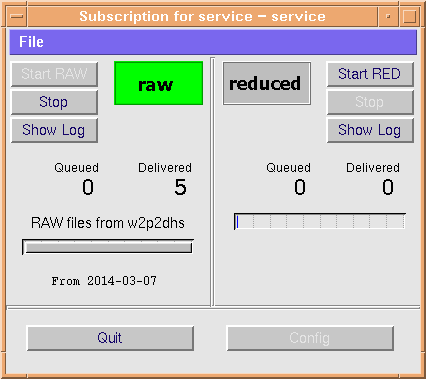
\includegraphics[width=\linewidth]{drs/datasubscriber.png}
\label{fig:datasubscriber}
}
\end{minipage}
\hspace{0.02\linewidth}
\begin{minipage}{0.48\linewidth}
\subfigure[\gls{feros} \texttt{data subscriber configuration window.}]{
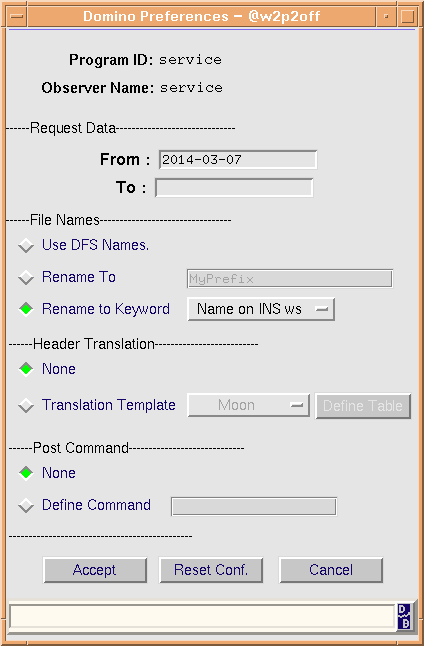
\includegraphics[width=\linewidth]{drs/datasubscriberconfig.png}
\label{fig:datasubconfig}
}
\end{minipage}
\caption{\gls{feros} Data Subscriber.}
\end{figure}

\subsection{Data won't show up}

If data taken with FEROS do not show up in the ESO archive and/or in the
FEROS DRS, you will need to restart processes on the data handling machine w2p2pl (username pipeline).

\procedure{Restart the data handler.}
\label{sec:DHrestart}
\begin{enumerate} 
    \item Go to screen \texttt{w2p2pl Pipline}
    \item In a terminal you will need to type some of the following
        \begin{enumerate}
            \item \texttt{dhsSubscribeControl start pipeline -backsince <date>}\\where <date> in the format YYYY-MM-DD is where you want to start again.
            \item (needed?) \texttt{pipelineControl stop}
            \item (needed?) \texttt{pipelineControl start}
            \item (needed?) \texttt{stopRBS}
            \item (needed?) \texttt{startRBS pipeline.config}
            \item \texttt{doControl stop}
            \item \texttt{doControl start wfi,feros}
        \end{enumerate}
\end{enumerate}

\newpage
\section{Startup issues}

\subsection{FEROS}
\label{sec:ferosstartuptimeout}
\begin{itemize}
  \item There is an error about process \texttt{feoControl} stating
      ``accepted PING but did not reply properly within 10000 msec'''
      \begin{itemize}
        \item Type \texttt{vccEnvStop -e \$RTAPENV}
        \item Type \texttt{vccEnvStart -e \$RTAPENV}
        \item Redo the full startup procedure
      \end{itemize}
 \item There is a problem with the FEROS telemetry at TCS (window should show some graphs, Fig.~\ref{fig:tcstelemetry}), run Procedure~\ref{proc:telemetry}
\end{itemize}

\procedure{Activate FEROS or WFI telemetry}
\label{proc:telemetry}
\begin{enumerate}
    \item Go to FEROS or WFI screen
    \item Open or locate a terminal and type \texttt{fcdTelemetry \&}
    \item On the emerging \texttt{FIERA - Telemetry} GUI, press \texttt{Start}
    \item Close the GUI
    \item Go to TCS screen
    \item Close the \texttt{ESO 220 General Telemetry Panel}
    \item Open or locate a terminal and type \texttt{sciops2p2Telemetry \&}
\end{enumerate}

\begin{figure}[t!]
\begin{minipage}{0.48\linewidth}
\subfigure[Telemetry window at \gls{tcs}, should show some graphs normally.]{%
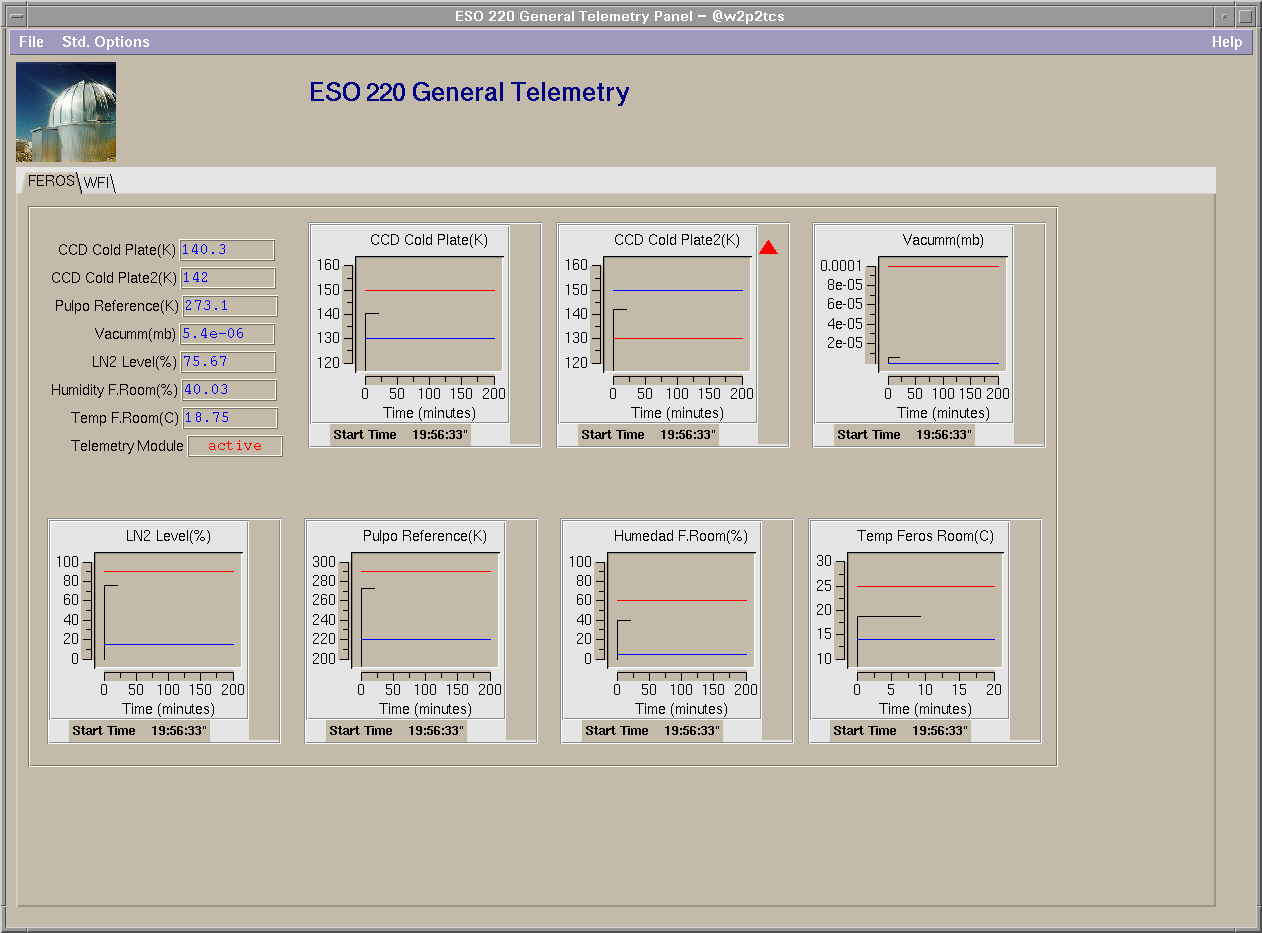
\includegraphics[width=\linewidth]{tcs/TCS-telemetry.png}
\label{fig:tcstelemetry}
}
\end{minipage}
\hspace{0.02\linewidth}
\begin{minipage}{0.48\linewidth}
\subfigure[\gls{feros} telemetry window.]{
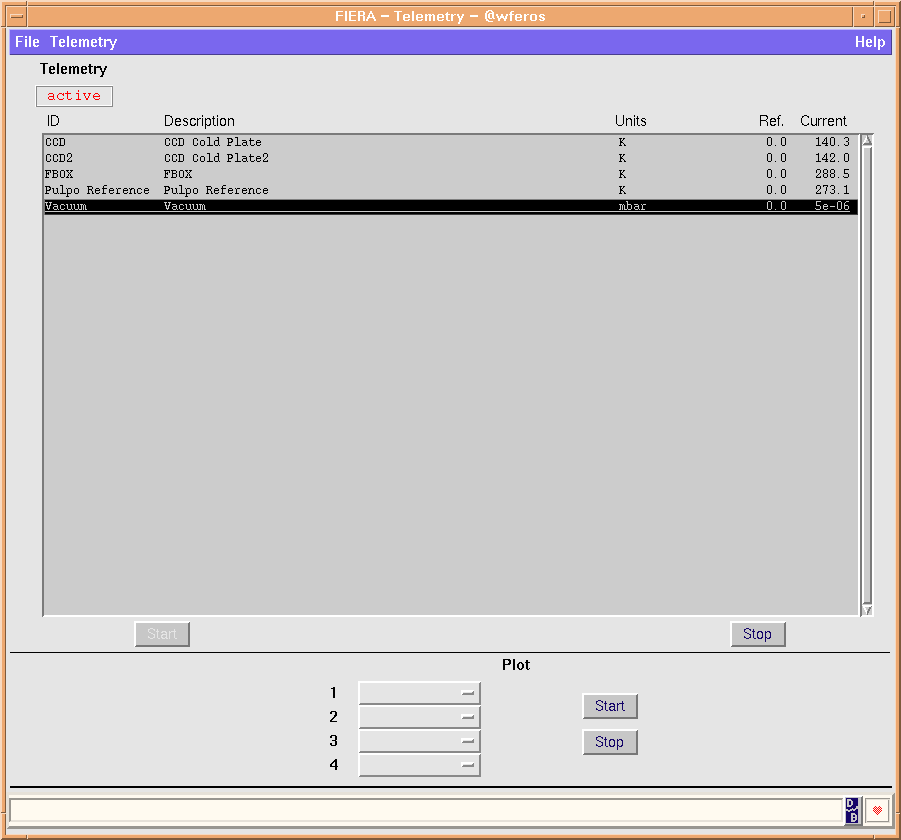
\includegraphics[width=\linewidth]{feros/FEROS-telemetry.png}
\label{fig:ferostelemetry}
}
\end{minipage}
\caption{Telemetry window.}
\end{figure}

\subsection{WFI}

The commonest issues are:
\begin{itemize}
  \item \gls{tcs} is \texttt{OFF} after startup on the Control Panel\\
   This is harmless. Use menu \texttt{Gen. Options} $\rightarrow$ \texttt{Refresh Database Events}.
  \item WFI startup stops with an error during \texttt{WFI Init/Online}\\
       It most likely requires a power cycle of the WFI electronics, see below.
\end{itemize}

\begin{figure}[ht]
	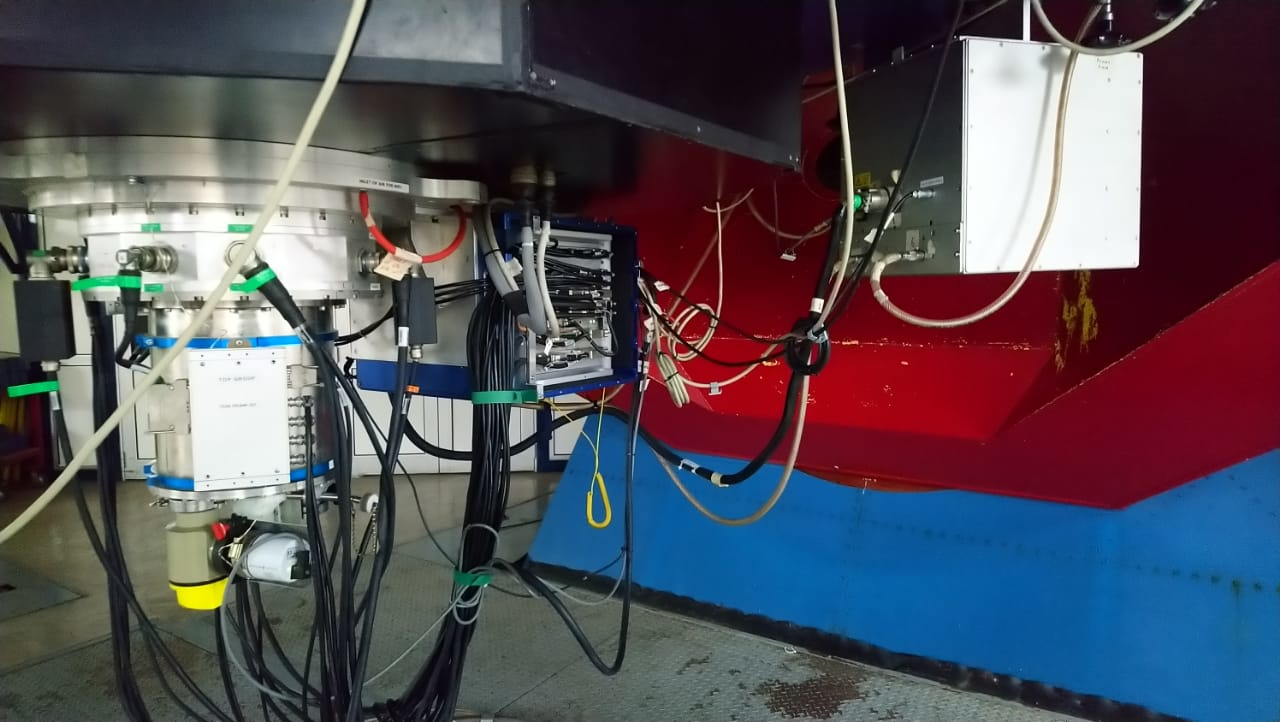
\includegraphics[width=0.45\linewidth]{wfi/wfielectronics-1.png}
	\hglue 0.02\linewidth
	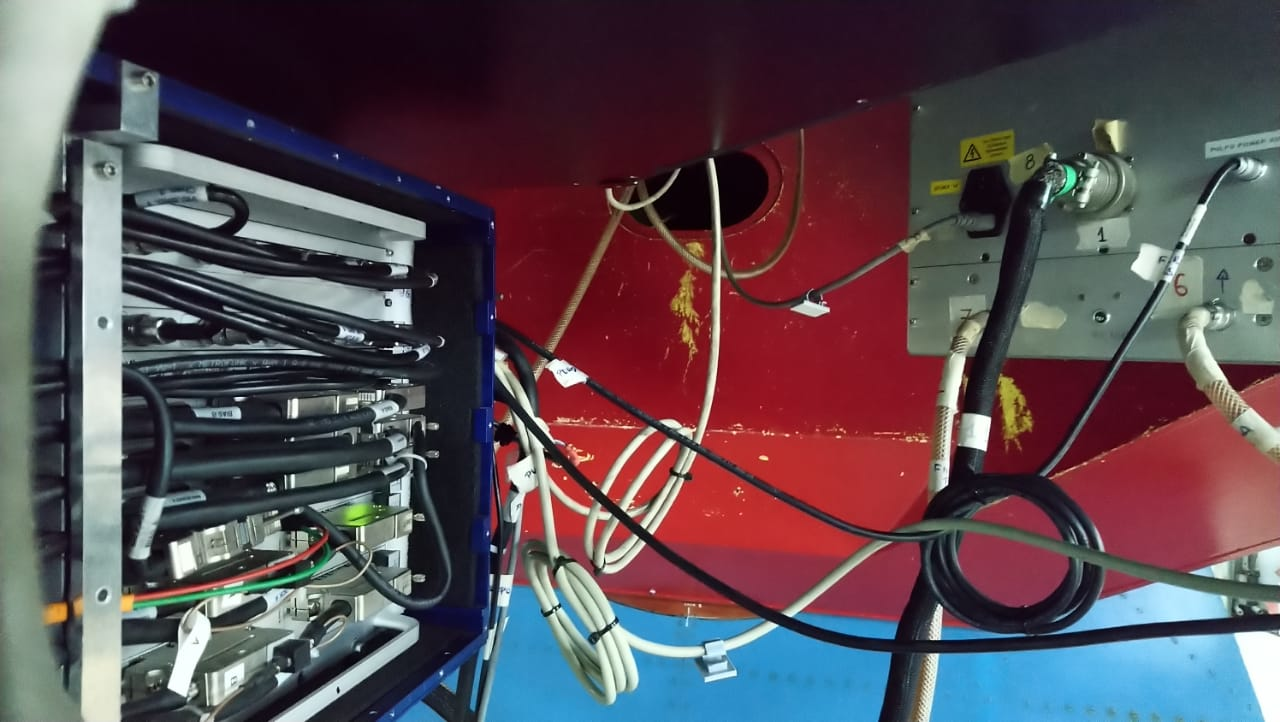
\includegraphics[width=0.45\linewidth]{wfi/wfielectronics-2.png}
	\caption[WFI electronics: power cycle button and boards]{WFI electronics.  The box on the right controls the power and can be used to power cycle.
The box on the left contains the electronics boards that one may need to unplug and replug.}
	\label{fig:wfielectronics}
\end{figure}

\procedure{Fix WFI init error}
\begin{enumerate}
  \item Determin whether WFI passes the hardware self-test
    \begin{enumerate}
	\item Locate or open a \texttt{logMonitor}
	\item If it was not active, choose to inspect the last 500 lines
	\item Find red error ``Failed to dispatch command for camera LOADED OK''.
	\item Lines below and above contain ``C40 ping failed'' and ``Could not download \gls{fiera} config''
	\item You can also check directly whether WFI passes the self-test\\
              In a terminal, type \texttt{rsh -l fcdrun wwffcd "export DISPLAY=\$DISPLAY; fcdtestseq"}
    \end{enumerate}
  \item\label{list:wfionline:reboot} Reboot the \gls{fiera} workstation
	\begin{enumerate}
		\item In a terminal, type \texttt{rsh -l fcdrun wwffcdd reboot}
	        \item Wait for 1--2 minutes for it to get back online\\
		      You may check in a terminal using \texttt{ping wwffcd}
	\end{enumerate}
  \item If WFI doesn't pass the self-test, power cycle the WFI electronics 
	\begin{enumerate}
		\item Go to the telescope floor
		\item Locate the WFI power unit close to the FIERA electronics
			(Fig.~\ref{fig:wfielectronics})
		\item Switch it off
                \item Wait for 30 seconds.\\
                      (On a 2nd or 3rd attempt, you may try to unplug/replug the electronics boards if you dare.)
		\item Switch it on.
	\end{enumerate}
  \item  If WFI passes the self-test, do a restart of the \gls{fiera} 
        \begin{enumerate}
		\item In a terminal, type \texttt{fcdCtrl}
                \item On the emerging GUI, click \texttt{Shutdown}
                \item On the emerging GUI, click \texttt{Startup}
		\item Wait for \gls{fiera} to restart (1 min ?)
        \end{enumerate}
  \item\label{list:wfionline:restart} Do a full WFI restart (see Proc.~\ref{proc:startup} point~\ref{list:wfistartup} and Fig.~\ref{fig:wfi-restart})
  \item You may have to redo steps \ref{list:wfionline:reboot}--\ref{list:wfionline:restart} until WFI can finish the full restart.
\end{enumerate}


\subsection{Hydraulics cannot be switched on/off}
\label{sec:hydr-loc}
If you see that the \texttt{Loc/Re} button is red on the \texttt{2.2m Auxiliary Funct} on the Windows computer, it means that the hydraulics system is for local control in the dome.

You need to go to the dome.

\procedure{Set the hydraulics for remote control}
\begin{enumerate}
   \item Go to the dome.
   \item Locate the gray 1.5-metre-high \gls{adam} rack (Fig.~\ref{fig:dome}).
   \item Locate the switch for \texttt{ADAM Remote} / \texttt{Local} (Fig.~\ref{fig:dome-adam}, lower left).
   \item Put it towards \texttt{ADAM Remote}.
\end{enumerate}

\section{TCS issues}
\subsection{Start-up fails with l2p2cam error}
\begin{figure}
    \centering
    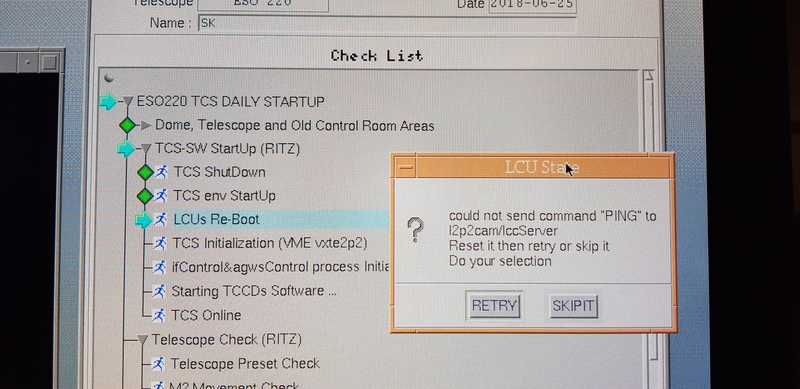
\includegraphics[width=\linewidth]{tcs/TCS-l2p2cam.jpg}
    \caption{When TCS restart fails to reboot the FEROS AG LCU}
\end{figure}

If the start-Up stalls with error \texttt{could not send command "PING" to l2p2cam/lccServer}, you probably need to hard reboot the  \gls{feros} \gls{ag} \gls{lcu} in the dome, but try a software reboot first to save time.

\procedure{Fix FEROS AG LCU during start-up}
    \begin{enumerate}
        \item Try a software restart of the \gls{feros} \gls{ag} \gls{lcu} (likely to fail).
        \begin{enumerate}
            \item On the \gls{tcs} screen, find or open a terminal
            \item Type \texttt{rsh l2p2cam reboot}\\
                  If it gives an error, proceed to step~\ref{lab:startupfag2}
            \item Wait for 1--2 min for the reboot to complete 
            \item Check that the LCU is up using \texttt{ping l2p2cam}
            \item Press \texttt{CONTINUE} in the Start/Shutdown panel\\
                  If it gives the same error popup, proceed to step~\ref{lab:startupfag2}. 
        \end{enumerate}
        \item\label{lab:startupfag2} Go to the dome and try, in that order (see Procedure~\ref{proc:restartfag}).
            \begin{enumerate}
            \item A hard reset of the LCU
            \item A power cycle of the LCU
            \end{enumerate}
    \end{enumerate}

\subsection{Start-up fails with telescope not initialised}

If the start-up stalls with \texttt{telescope not initialised}, you probably forgot to switch the hydraulics and/or drives on or the telescope was not parked at zenith. 

\procedure{Fix the telescope not initialized popup} 
\begin{enumerate}
    \item Ensure hydraulics and drive are on
        \begin{enumerate}
            \item Locate the \gls{domefunc} tab on screen \texttt{Dome webcam \& hydraulics}. 
            \item Check that the \texttt{Hydr} and \texttt{Drives} buttons are green.
            \item If not, switch the hydraulics and drives on (step~\ref{lab:hydron} in Procedure~\ref{proc:startup}).
        \end{enumerate}
    \item Manually initialise the telescope
        \begin{enumerate}
            \item\label{lab:notinit1} 
                In a terminal type \texttt{\home/bin/telinit}
            \item If an error reads "cannot initialise the 
                telescope at more than 45 degrees from zenith"
                \begin{enumerate}
                     \item Go to the dome and manually park it (Procedure~\ref{proc:park}). 
                     \item Repeat step~\ref{lab:notinit1}
                \end{enumerate}
            \item Wait for 2--3 min for initialisation to complete.
        \end{enumerate}
    \item On the error popup, press \texttt{SKIPIT}
\end{enumerate}

\subsection{Quick TCS restart}
\label{sec:tcsrestart}

Many \gls{tcs} issues are solved by a fast restart, with a time loss of $\approx 10$~min. Before, it is important move the telescope to zenith since one cannot initialize it later if the telescope is at $\le$ 45 degrees above the horizon.

\procedure{Quick TCS restart}
\begin{itemize}
 \item Preset to zenith
    \begin{itemize}
	\item On the \gls{tcs} setup panel (Fig~\ref{fig:tcssetup}), click \texttt{Zenith} under \texttt{Fixed Presets}.
        \item Alternatively, if panel is frozen, type \texttt{\home/bin/presetzenith} in a terminal.
    \end{itemize}
 \item Execute the fast restart.\\
       Type \texttt{e2p2NewStartUp} and wait for it to complete.
 \item Initialise the telescope\\
       On the \gls{tcs} setup panel (Fig~\ref{fig:tcssetup}) press \texttt{Initialize} under \texttt{Telescope}.
\end{itemize}

\subsection{No connection with VME}
If the TCS Control Panel indicates ``No connection'' in red, just below \texttt{VME messages}, you can try the following:

\begin{figure}
\centering
\subfigure[Remote/local pointing control]{%
\includegraphics[width=0.33\linewidth]{dome/dome-tel-local-to-remote.jpg}%
\label{fig:tel-remote}%
}%
\subfigure[Reboot of the VME]{%
\includegraphics[width=0.33\linewidth]{dome/dome-vme-reboot.jpg}%
\label{fig:vme-reboot}%
}
\subfigure[VME monitor]{%
\includegraphics[width=0.33\linewidth]{dome/dome-vme-monitor.jpg}%
\label{fig:vme-monitor}%
}
\caption[VME rack in the computer room of the telescope building]{VME rack in the computer room of the telescope building 
\emph{Left:} to
manually point the telescope to zenith, you need to switch away from 
the yellow 'd' label. \emph{Centre:} To hard reboot the VME, press the small red/pinkish reset button. \emph{Right:} the VME monitor with the ``end of boot script'' after a reboot.}
\end{figure}

\procedure{Solve the connection issue with the VME}
\begin{enumerate}
    \item If you just switched hydraulics on, wait for a few minutes to see
        if connection is back.
    \item Do a remote reboot of the VME.\\
          Type \texttt{lccBoot lte2p2} in a terminal.
    \item Do a manual reboot of the VME in the dome.
    \begin{enumerate}
        \item Go to the computer room of the telescope enclosure.
        \item Locate the VME (Fig.~\ref{fig:computer-room}) in front of the entrance, slightly to the left.
        \item Press the small red/pinkish button (Fig.~\ref{fig:vme-reboot}).
        \item Locate the VME monitor, behind you if you face the VME.
        \item Wait for boot sequence to finish with ``end of boot script'' (Fig.~\ref{fig:vme-monitor})
    \end{enumerate}
\end{enumerate}

A quick restart the \gls{tcs} (Sect.~\ref{sec:tcsrestart}) is generally needed right after a reboot of the VME.

\subsection{TCS is OFF on an instrument}
The Control Panel of an instrument the TCS is in the state \texttt{OFF}. You should check the corresponding modules on the TCS Status panel.  If red, try to bring them \texttt{ONLINE}.

\subsection{Telescope doesn't take focus orders}

\procedure{Fix telescope focus issues}
\begin{itemize}
  \item \textit{(\gls{wfi})} OB stalls when focus order is sent by \gls{bob}.\\
        Set it manually from the \gls{tcs} main panel (Fig.~\ref{fig:tcs})
  \item \textit{(\gls{feros})} Focus is not corrected after insertion of the ADC.\\
        See Sect.~\ref{sec:focusadc}.
  \item Focus cannot be set from the \gls{tcs} main panel.\\
        Restart the \gls{tcs}, see Sect.~\ref{sec:tcsrestart}.
\end{itemize}

\subsection{TCS Setup panel is stuck}

If you need to close when the panel is stuck, a few command lines are available in \texttt{/home/tcs/bin}: \texttt{closemirror}, \texttt{closeslit}, \texttt{presetzenith}, \texttt{domemanual}. 

\procedure{Unstuck the TCS Setup panel}
\label{proc:unstuckTCSpanel}
\begin{enumerate}
  \item In a terminal type \texttt{killall rs232}\\
        If ``no process killed'' appears, this procedure will not be useful.
  \item If the panel gets stuck again quickly (10--20 s), a restart of the TCS usually fixes the issue. 
\end{enumerate}

\subsection{Main mirror cover cannot be moved}
\begin{figure}
\centering
\includegraphics[width=0.7\linewidth]{dome/dome-adam.jpg}
\caption{Controlling the hydraulics and mirror cover.}
\label{fig:dome-adam}
\end{figure}

If the \texttt{Main Mirror Cover} state in the \texttt{TCS Setup Panel} says
\texttt{LOCAL} you need to go to the dome, close it, and set it
to remote control.

If the \texttt{Main Mirror Cover} state in the \texttt{TCS Setup Panel} stays in
\texttt{MOVING} whatever order you send, you need to go to the dome, set it for local control, close it, and set it to remote control.
 

\procedure{Manually close the main mirror cover}
\begin{enumerate}
   \item Go to the dome
   \item Locate the gray 1.5-metre-high ADAM contol box (Fig.~\ref{fig:dome}).
   \item Locate the \texttt{Main Mirror Cover} controls (Fig.~\ref{fig:dome-adam}, upper right) 
   \item If the mirror was \texttt{MOVING}, press the yellow \texttt{Local/Remote} button.
   \item Press the red \texttt{Mirror Close} button.
   \item If any noise is heard, wait for the cover to be closed.
   \item Press the yellow \texttt{Local/Remote} button.
\end{enumerate} 


\subsection{Dome doesn't move}
\begin{figure}
\centering
\includegraphics[width=0.6\linewidth]{dome/dome-control.jpg}
\caption{Local control of the dome}
\label{fig:dome-control}
\end{figure}

If the \texttt{Dome Status} is \texttt{Local} on the \texttt{TCS Control Panel}, it means that the dome is for local control from the dome.

You need to go to the dome.

\procedure{Set the dome for remote control}
\begin{enumerate}
   \item Go to the dome.
   \item Locate the dome controls (Fig.~\ref{fig:dome}), placed on the wall opposite to the entrance.
   \item On the dome controls (Fig.~\ref{fig:dome-control}) turn the control from local to remote
\end{enumerate}

\subsection{Dome slit and telescope are not aligned}
For small zenithal angles, it is a normal setting since the telescope is not exactly at the centre of the dome.  If you need to avoid the wind you need to orient the dome manually but be weary of vignetting!

\section{GROND issues}
\subsection{GROND M3 is stuck}
\begin{figure}[t!]
\begin{minipage}{0.28\linewidth}
\subfigure[ccsei window.]{%
\includegraphics[width=\linewidth]{grond/unstucking-grond-m3-0.png}
\label{fig:ccs}
}
\end{minipage}
\hspace{0.02\linewidth}
\begin{minipage}{0.7\linewidth}
\subfigure[M3 in the database]{
\includegraphics[width=\linewidth]{grond/unstucking-grond-m3.png}
}
\end{minipage}
\caption{Writing the M3 position in the database}
\label{fig:ccs-grondM3}
\end{figure}

\begin{figure}
\includegraphics[width=0.6\linewidth]{dome/dome-grond-m3-box.jpg}
\caption{The GROND mirror and main cover control box.}
\label{fig:grondM3-box}
\end{figure}

If \gls{grond} M3 mirror cannot be moved with the \texttt{grondM3} command try in order the items of the procedure below.

\procedure{Unlocking the grond M3 mirror} 
\begin{itemize}
  \item Switch back-and-forth using \texttt{grondM3 WFI} and \texttt{grondM3 GROND}.
  \item Write the mirror position in the database (Fig.~\ref{fig:ccs-grondM3})
    \begin{enumerate}
      \item In a terminal type \texttt{ccsei}
      \item Click on \texttt{CCS database monitor} 
      \item Look down \texttt{Appl\_data $\rightarrow$ GROND 
        $\rightarrow$ ICS  $\rightarrow$ DEVICES  $\rightarrow$ M3}.
      \item Select checkbox \texttt{Enable Editing}
      \item set \texttt{newPos} value to 2 for GROND position or 0 for WFI.
      \item Check on GROND control that mirror indeed moves.
      \item Close the GUI.
    \end{enumerate}
  \item Reset the mirror from the dome.
    \begin{enumerate}
       \item In the dome, locate the M3/MC box below the main mirror (Fig.~\ref{fig:dome}).
       \item On the box (Fig.~\ref{fig:grondM3-box}), press the grondM3 WFI button.
    \end{enumerate}
\end{itemize}

\subsection{GROND OB only crashes with TCS on}

It is a very tricky problem, randomly solved by a string of last resort reboots of GROND and TCS restarts. 

\subsection{GROND IR exposure won't start}

\begin{figure}
\centering
\subfigure[GROND \gls{irace} box]{%
\includegraphics[width=.49\linewidth]{dome/dome-grond-irace.jpg}%
}%
\hspace{0.01\linewidth}%
\subfigure[GROND IRACE switch]{%
\includegraphics[width=.49\linewidth]{dome/dome-grond-irace-switch.jpg}%
}%
\caption[The GROND IRACE box]{The GROND infrared electronics (\gls{irace}) box below the main mirror of the telescope.  The power switch
is located towards the pier.}
\label{fig:grond-irace}
\end{figure}

An OB starts with the optical exposure but nothing happens in the infrared and
the OB stalls. If \texttt{grondFM} doesn't solve the issue, this may need a full reset of the \gls{irace} (IR electronics).
 
\procedure{Deep reset of GROND IRACE (verify this!)}
\label{proc:iracerestart}
\begin{enumerate}
  \item In a GROND terminal, do \texttt{grinsStop} as user  \texttt{grondmgr}.
  \item Go to the computer room of the telescope building.
  \item Locate the \gls{irace} workstation (Fig.~\ref{fig:computer-room}) and shut it down.
  \item Go to the dome 
  \item Locate the power switch of the \gls{irace} box (Fig.~\ref{fig:grond-irace}) below the main mirror.
  \item Switch it off for 10 seconds then on again.
  \item Go back to the computer room and start the IRACE workstation.
  \item Go back to the control room and reboot the GROND workstation.
  \item Do \texttt{\home/bin/lastResortBeforeReboot.sh} as user \texttt{grondmgr}
  \item Reboot GROND workstation.
  \item Do \texttt{\home/bin/lastResortAfterReboot.sh} as user \texttt{grondmgr}
  \item Put the instrument \texttt{ONLINE} in the GROND panel
  \item Do \texttt{grondSHUTER \&\& grondFM}
  \item close and open bob
\end{enumerate} 

\section{Freezing issues}

\subsection{Mouse pointer does not move}
This is common on the \gls{wfi} screens.

\procedure{Recover the mouse pointer}
\begin{enumerate}
    \item Power cycle the black Intel box connected to the failing screen.\\
          Press power button for 5\,s, wait 5--10\,s, switch it on, wait for
          start-up (1--2\,min)
    \item Log in\\ 
          For WFI, user wfi (other logins in Table~\ref{fig:computers}).
    \item Open the panels from a terminal.\\
          For WFI, type \texttt{\home/bin/openPanels.sh}.
\end{enumerate}

\section{Pointing issues}

\subsection{Pointing is incorrect}
\label{sec:trouble:pointing}
\begin{table}[!bt]
\centering
\caption{Pointing model parameters for each instrument, as of November 2015.}
\label{tab:pointingmodelcoeff}
\small
\begin{tabular}{lrrr}
\hline\hline
Parameter & FEROS      & GROND     & WFI\\\hline
ID        & $-183.81$  & $-230.04$ & $-157.69$\\
IH        & $  72.92$  & $ -20.23$ & $  94.11$\\
CH        & $ 136.07$  & $  28.89$ & $  31.41$\\\hline
NP        & \multicolumn{3}{r}{$17.13$}\\
ME        & \multicolumn{3}{r}{$-113.61$}\\
MA        & \multicolumn{3}{r}{$2.22$}\\
FO        & \multicolumn{3}{r}{$91.83$}\\
TX        & \multicolumn{3}{r}{$-26.92$}\\
HCEC      & \multicolumn{3}{r}{$-18.57$}\\
HCES      & \multicolumn{3}{r}{$-22.55$}\\\hline
\end{tabular}
\end{table}

After doing the pointing with \gls{wfi} the target is not close to the central position (4150,3950).  Also, it can happen during an observation with any instrument during the night that the object is not centred where it should.

\procedure{Fix WFI pointing issues.}
\begin{enumerate}   
    \item If not done, check the right instrument is selected on the \gls{tcs} \texttt{Status Panel}
        (Fig.~\ref{fig:tcsstatus}).
    \item Check if the current Pointing Model parameters in Table.~\ref{tab:pointingmodelcoeff} for \gls{wfi} are selected on the \gls{tcs} Setup Panel (blue numbers in the bottom right-hand panel of Fig.~\ref{fig:tcssetup}). Typically
        the first three values ID, IH, CH are 0 because of a database issue.\\
        In a hurry:
        \begin{itemize}
            \item Reset the database values\\
                  In a terminal type \~{}\texttt{/bin/fixPointing.sh}\\
                  (Note: it can be done manually using \texttt{ccseiDb})
            \item Select the instrument again
        \end{itemize}
        Otherwise, a quick TCS restart will generally solve the issue.
    \item Check that the Sidereal time on the \gls{tcs} Control Panel is fine.\\
      It should be withing seconds of the actual one.  You can get it from
      the digital clock in the control room using a switch on its right.\\
      If not, you need to go to the dome and reboot the VME.
    \item Otherwise, it might be a problem with the \gls{tcs}.\\ 
       Try a quick \gls{tcs} restart (Sect.~\ref{sec:tcsrestart}).
\end{enumerate}  

\subsection{Telescope is stuck at low elevation}

\begin{figure}
\centering
\subfigure[Location of the joystick]{%
\includegraphics[width=0.6\linewidth]{dome/dome-tel-joystick-location}%
}%
\hspace{0.03\linewidth}%
\subfigure[Joystick]{%
\includegraphics[width=0.3\linewidth]{dome/dome-tel-joystick}%
}
\caption{The ``joystick'' can be used to manually point the telescope.}
\label{fig:tel-joystick}
\end{figure}

If telescope goes out of safe zone, reaching 20 degrees elevation, a too high hour angle, it will be stuck (by software). It also occurs if a restart or a reboot of the VME is done when the telescope points lower than 45 degrees.

In that case, the telescope should be parked to zenith manually.

\procedure{Preset manually to zenith.}
\label{proc:park}
\begin{enumerate}   
    \item Go to the computer room in the telescope enclosure.
    \item Locate the VME rack (Fig.~\ref{fig:computer-room}).
    \item On the VME, set the switch away from d (Fig.~\ref{fig:tel-remote}).
    \item Go to the dome and find the joystick (Fig.~\ref{fig:tel-joystick}).
    \item Using the controls put the telescope approximately to zenith.
    \item Go to the computer room in the telescope enclosure.
    \item On the VME rack, set the switch to d.
    \item Go to the control room below the dining room.
    \item Initialise the telescope\\
          Click \texttt{Initialize} below \texttt{Telescope}  in \texttt{the TCS Setup Panel}
\end{enumerate}

\section{Web pages}

\subsection{2.2m Environmental Monitor stuck}
If the 2.2m Environmental Monitor is stuck.

\procedure{Restart the 2.2m environmental monitor}
\begin{enumerate}
  \item Go to screen \texttt{Telescope Control Software}.
  \item In a terminal, execute command \texttt{e2p2StartEnvMon}
  \item After a few minutes refresh \url{http://www.ls.eso.org/lasilla/sciops/2p2/EnvMon}.
\end{enumerate}

\subsection{All sky camera}
If the all sky camera LASCAM is stuck
\begin{enumerate}
  \item Use the Danish 1.54m camera at \url{http://allsky-dk154.asu.cas.cz/}
  \item Ask an ESO TIO to restart LASCAM.
\end{enumerate}

\section{ESO database issues}

\procedure{Data do not appear in the database}
\begin{enumerate}
   \item Wait for one or two days after the data is taken because there may be a lag
   \item If all observations including the calibrations do not show up,
         you can restart the data handler\\
         See Procedure~\ref{sec:DHrestart}
   \item If only a particular set of observations loaded directly from bob
         are impacted, check that the PID is correct
         \begin{enumerate}
           \item Open the OBs (usually in OBD directory on bob machine)
           \item Check that the ESO PID has a valid format.
           \begin{itemize}
               \item Science OBs must start with a leading
                 zero for science PIDs, e.g. 0103.A-9001(A)
               \item Calibration OBs should not have a leading zero, e.g 60.A-0040(Z) 
           \end{itemize}
           \item Check that the ESO PID has been assigned 
              \begin{enumerate}
                \item Open the ESO Observing Schedule Query Form\\
                      \url{http://archive.eso.org/wdb/wdb/eso/sched\_rep\_arc/form}
                \item Fill telescope (\texttt{La Silla -{}- 2.2 m}) and period 
                \item Click \texttt{Search}
              \end{enumerate}
           \item If not assigned or invalid format, contact User Support Department at ESO to fix it.
     \end{enumerate}
   \item Data taken as \texttt{TEST} (daily checks) do not apear in the archive.
\end{enumerate}


%%%%%%%%%%%%%%%%%%%%%%%%%%%%%%%%%%%%%%%%%%%%%%%%%%%%%%%%%%%%%%5


\chapter{Main systems}
\label{compo}


\begin{figure}[!ht]
\centering
\includegraphics[width=.85\linewidth]{tcs/TCS.png}
\caption[Main panel of the telescope control software]{The \gls{tcs} main panel allows to perform guiding with \gls{wfi} and to manually preset or offset.}
\label{fig:tcs}
\end{figure}

\begin{figure}[!ht]
\centering
\includegraphics[width=.85\linewidth]{tcs/TCS-setup.png}
\caption[Setup panel of the telescope control software]{The \gls{tcs} setup panel allows to open and close the dome, main
mirror cover and setup the dome rotation.  Additionally, fixed presets
to zenith and flat screen can be sent.}
\label{fig:tcssetup}
\end{figure}

\section{Telescope control software}

The main panel of the \gls{tcs} (Fig.~\ref{fig:tcs}) gives a summary of focus,
guiding, and pointing. The rose diagram gives telescope position, slit
orientation (symbol just outside the outermost circle), Moon position (yellow
circle), and some other info (green arrow). Telescope status and dome status
indicate whether telescope is presetting, slewing, guiding, or offsetting.  The
panel also allows some interaction.  The \gls{tcs} setup panel
(Fig~\ref{fig:tcssetup}) allows more interaction, in particular concerning
closing and opening.

\subsection{Manual preset}  
\label{manualpreset}


The presetting area  of the main \gls{tcs} panel (Fig.~\ref{fig:tcs}) allows manual
preset, which is used for flat fields and \gls{wfi} focus.  Catalogues can be loaded
with \texttt{CalSelect}, in particular EmptyFields for flat fielding. The item
of the catalogues is selected with \texttt{Top}, \texttt{Up}, \texttt{Dwn},
\texttt{Bot} before \texttt{Preset} is clicked.

\subsection{Manual offset}
\label{manualoffset}

The virtual handset area of the main \gls{tcs} panel (Fig.~\ref{fig:tcs})
allows to give an offset which is used when looking for a guide star on
\gls{grond} or centring a target on the \gls{feros} fibre when guiding with the
\gls{wfi} \gls{ag}.  An offset is done by clicking \texttt{Offset} and
selecting \texttt{combined offset} (useful when guiding).  Offset steps are
input with \texttt{Store}, then the racquet in the centre (\texttt{$-$RA},
\texttt{$+$RA}, \texttt{$-$Decl}, \texttt{$+$Decl}) can be used.

\subsection{Autoguider}
\label{autoguider}

\begin{figure}[!ht]
\centering
\includegraphics[width=.85\linewidth]{tcs/TCS-AG.png}
\caption[WFI autoguider]{The \gls{ag} field is displayed on the \gls{tcs} \gls{rtd} (left) where the
 reference star can be picked (using lower right window).} 
\label{fig:tcsag}
\end{figure}
The \gls{ag} in the \gls{tcs} can be used for \gls{wfi} and \gls{feros} observations.

The \gls{ag} Field Acquisition and Autoguider areas of the main \gls{tcs} control panel
(Fig.~\ref{fig:tcs}) give control over \gls{wfi} \gls{ag}.  The buttons of
interest are \texttt{Retrieve field} (to probe the \gls{ag} field, displayed
in Fig.~\ref{fig:tcsag}), \texttt{Box to
star} (to start the guiding when a guide star has been picked) and \texttt{Off}
(to turn off the \gls{ag}).  Tuning of the \gls{ag} (e.g. integration time) can be done 
on  the Autoguider area of the \gls{tcs} setup panel (Fig.~\ref{fig:tcssetup}).

Note that guiding must be set \texttt{Off} at the end of a \gls{feros} observation
using the \gls{wfi} \gls{ag}. The buttons \texttt{Stop Monitoring} and \texttt{Start Monitoring} are
useful after a change of filtres on the same field, for they avoid
a \texttt{Retrieve Field}.

Differential guiding can be set, but a particular care should be paid
to units (here arcsec/hour).


\begin{figure}[!ht]
\centering
\includegraphics[width=.6\linewidth]{tcs/TCS-status.png}
\caption[Status window of the telescope control software]{The TCS status window is mostly used to switch the pointing model
between instruments.}
\label{fig:tcsstatus}
\end{figure}


\begin{figure}[!ht]
\centering
\includegraphics[width=.18\linewidth]{tcs/TCS-auxfunc-menu-1.png}%
\includegraphics[width=.18\linewidth]{tcs/TCS-auxfunc-menu-2.png}
\hglue 4em
\includegraphics[width=.4\linewidth]{tcs/TCS-auxfunc.png}
\caption[Auxiliary functions of the telescope control software]{The \gls{auxfunc} panel (right) is opened using the menu
on the TCS machine (left). It is mostly used to switch the flat field 
lamp on and off, and to open or close the \gls{wfi} protective shutter.}
\label{fig:tcsauxfunc}
\end{figure}

\section{WFI}

\begin{figure}[!ht]
\centering
\includegraphics[width=.8\linewidth]{wfi/wfi-e2p2-os-gui.png}
\caption[WFI OS GUI]{The \gls{wfi} OS GUI can be used to change filtres manually or
take/abort CCD exposures.}
\label{fig:wfios}
\end{figure}

\begin{figure}[!ht]
\centering
\includegraphics[width=.8\linewidth]{wfi/wfi-state-manager.png}
\caption[WFI state manager]{The \gls{wfi} state manager holds information on telescope
focus, also used for \gls{feros}.}
\label{fig:wfistate}
\end{figure}

\begin{figure}[!ht]
\centering
\includegraphics[width=.8\linewidth]{wfi/wfi-general-state.png}
\caption[WFI general state panel]{The \gls{wfi} general state panel gives information
about exposure, filtres, and connection to \gls{tcs}.}
\label{fig:wfigen}
\end{figure}

\section{FEROS}

\begin{figure}[!ht]
\centering
\includegraphics[width=.8\linewidth]{feros/FEROS-Control.png}
\caption[FEROS control panel]{The \gls{feros} control panel gives information
about exposure, settings, lamps, and connection to \gls{tcs}.  Exposure times
can be switched.}
\label{fig:feroscon}
\end{figure}

\begin{figure}[!ht]
\centering
\includegraphics[width=.8\linewidth]{feros/FEROS-ICS.png}
\caption[FEROS instrument control software panel]{The \gls{feros} \gls{ics} is mainly used to change the mirror 
\texttt{mirr3} from and back to \gls{wfi}.}
\label{fig:ferosics}
\end{figure}


\section{GROND}

\begin{figure}[!ht]
\centering
\subfigure[\gls{grond} ``normal \gls{bob}'' with a test \gls{ob}.]{%
  \includegraphics[width=.49\linewidth]{grond/grond-bob.png}
  \label{fig:grondbob}
}\hfill
\subfigure[\gls{grond} control]{%
  \includegraphics[width=.49\linewidth]{grond/grond-control.png}%
  \label{fig:grondcon}
}
\caption{The main displays of \gls{grond}.}
\label{fig:grondmain}
\end{figure}

\begin{figure}[!ht]
\centering
\subfigure[\gls{grond} \gls{fiera} control panel (CCDs)]{%
  \includegraphics[width=.43\linewidth]{grond/grond-fiera.png}
  \label{fig:grondfiera}
}\hfill
\subfigure[\gls{grond} \gls{irace} control panel (IR detectors)]{%
  \includegraphics[width=.55\linewidth]{grond/grond-irace.png}%
  \label{fig:grondirace}
}
\caption{Control panels for the detectors.}
\label{fig:gronddet}
\end{figure}



\section{P2PP and OT}

\section{FEROS reduction software}

\section{Dome controls}
\begin{figure}[!ht]
\centering
\includegraphics[width=.7\linewidth]{dome/dome-auxfunc.png}
\caption{\gls{domefunc}.}
\label{fig:domefunc}
\end{figure}

\begin{figure}[!ht]
\centering
  \includegraphics[width=.7\linewidth]{dome/dome-webcam.png}%
\caption{\gls{webcam}}
\label{fig:webcam}
\end{figure}

\section{Computers}
Most components of the telescope can be accessed from any screen by using a graphical login: \texttt{tcs}, \texttt{cam} (guiders), \texttt{wfi}, \texttt{feros}, \texttt{dhs} (OBs), \texttt{astro} (pipelines), \texttt{grond}.  They are detailed in Fig.~\ref{fig:computers} and generally have the famous good seeing password. These machines need a reboot from time to time, using \texttt{reboot} as the normal user. 

For some tidying tasks or reboots, you need to root password (hint: pirate). 

Other components may need reboots, they are given in Table~\ref{tab:reboots}. 

\begin{table}
    \caption[Main workstations and users]{Computers one can use a graphical login for, from any screen, to get access to instruments and controls.  The password is the ``good seeing'' one shared by most  La Silla computers. The screen they are normally shown on and the relevant unix users are also given.  }
\label{fig:computers}
\centering
\begin{tabular}{lllll}
\hline
Computer         & Login    & User     & Monitor(s)                 & Description\\\hline\hline
\texttt{w2p2tcs} & tcs      & tcs      & Telescope Control Software & \gls{tcs}\\
                 & cam      & cam      & Autoguider GROND \& FEROS  & Autoguiders\\
\texttt{w2p2ins} & wfi      & wfi      & Wide Field Imager BOB      & WFI user\\
                 &          & wfimgr   & ---                        & manager account\\
\texttt{wferos}  & feros    & feros    & FEROS BOB                  & basic user\\
                 &          & ferosmgr & ---                        & manager account\\
\texttt{w2p2dhs} & dhs      & service  & p2p2 \& ot                 & service observations (ot)\\
                 &          & visitor  & p2pp \& ot                 & visitors (p2pp)\\
\texttt{w2p2off} & astro    & astro    & FEROS pipeline             & data \& pipelines\\
\texttt{w2p2pl}  & pipeline & pipeline & w2p2pl pipeline            & WFI/FEROS data handling\\       
\texttt{wgrond}  & grond    & grond    & GROND BOB / \gls{fiera} / \gls{irace}  & basic user\\
                 &          & grondmgr & ---                        & startup, \gls{bob}, commands\\
\hline
\end{tabular}
\end{table}

\begin{table}
\caption{Common passwords.}
\centering
\begin{tabular}{lll}
\hline
Component                 &  User name                                            & Password hint\\
\hline\hline
Graphical interface user  & tcs, cam, feros, wfi, grond, dhs, pipeline & .5a$\cdots$\\
Other users               & visitor, service                           & .5a$\cdots$\\
Instrument manager        & ferosmgr, grondmgr, wfimgr                            & pin2$\cdots$\\
Workstation administrator & root                                                  & 2be1$\cdots$\\
Remedy tickets            & 2p2                                                   & .5a$\cdots$\\
Observing tool            & 0                                                     & OHS4good\\
Dome auxiliary functions  &                                                       & .5a$\cdots$\\
p2pp for MPIA             & MPGUtility, MPGDDT                                    & MPG@$\cdots$\\
\hline
\end{tabular}
\end{table}

\begin{table}
\caption[Some useful reboots]{Reboots you may (will) have to do besides those of the aforementionned computers.}
\label{tab:reboots}
\centering
\begin{tabular}{lll}
\hline
Component   & Reboot command                       & Alternative reboots\\
\hline\hline
TCS LCU/VME & \texttt{lccBoot lte2p2}              & \texttt{rsh vxte2p2 reboot}\\ 
            &                                      & Reset button, VME rack, computer room at telescope$^\ast$\\
\hline
WFI FIERA   & \texttt{lccBoot wwffcd}$^\star$      & \texttt{rsh -l fcdrun wwffcd reboot}\\
\hline
FEROS LCU   & \texttt{lccBoot lfeics1}             & FEROS ICS, menu \texttt{LCU} $\rightarrow$ \texttt{Reboot}\\
            &                                      & \texttt{rsh -l fcdrun lfeics1 reboot}\\
FEROS AG    & \texttt{lccBoot w2p2cam}             & \texttt{rsh l2p2cam reboot}\\
            &                                      & Reset button, rack, FEROS room at telescope$^\ast$\\
            &                                      & Unplug rack, FEROS room at telescope$^\ast$\\
FEROS FIERA & \texttt{lccBoot wfefcd}$^\star$      & \texttt{rsh -l fcdrun wfefcd reboot}\\
\hline
GROND FIERA &                                      & \texttt{rsh root@wgrccd reboot}\\
            &                                      & Power switch, FIERA WS, computer room at telescope$^\ast$\\
GROND IRACE &                                      & \texttt{rsh root@wgrdcs reboot}\\
            &                                      & Power switch, IRACE WS, computer room at telescope$^\ast$\\
GROND AG    & \texttt{lccBoot w2p2agr}             & \texttt{rsh l2p2agr reboot}\\
\hline
User WS     & \multicolumn{2}{l}{call at Paranal 5959 to reboot uws2p2, first close all terminals}\\
\hline
\multicolumn{3}{l}{$^\star$ Untested.\quad $^\ast$ Manual reboot needed if soft fails.}\\
\hline
\end{tabular}
\end{table}

\setglossarystyle{altlist}
\printglossaries
\addcontentsline{toc}{chapter}{\textcolor{ocre}{Glossary}}
%\chapter*{Bibliography}
%\addcontentsline{toc}{chapter}{\textcolor{ocre}{Bibliography}}
%\section*{Books}
%\addcontentsline{toc}{section}{Books}
%\printbibliography[heading=bibempty,type=book]
%\section*{Articles}
%\addcontentsline{toc}{section}{Articles}
%\printbibliography[heading=bibempty,type=article]

%----------------------------------------------------------------------------------------
%	INDEX
%----------------------------------------------------------------------------------------

%\cleardoublepage
%\setlength{\columnsep}{0.75cm}
%\addcontentsline{toc}{chapter}{\textcolor{ocre}{Index}}
%\printindex

%----------------------------------------------------------------------------------------

\end{document}
